
\chapter{Аффинные алгебры Ли}
\label{cha:affine-lie-algebras}
Аффинные алгебры Ли - это естественное обобщение простых конечномерных алгебр Ли. Они возникают при изучении различных физических моделей, например, моделей Весса-Зумино-Новикова-Виттена в конформной теории поля и интегрируемых спиновых цепочек. 
\section{Введение. Простые алгебры Ли.}

\label{sec:intro-simple-lie-algebras}

{\it Алгебра Ли} $\gf$ -- это векторное пространство с билинейной операцией $[\cdot,\cdot]:\gf\otimes\gf\to \gf$, которая называется  {\it скобкой Ли или коммутатором}. Если выбрать некоторый  $X_{i}$ в $\gf$, то коммутационные соотношения можно задать при помощи  {\it структурных констант} $C_{ijk}$:
\begin{equation}
  \label{eq:1}
  [X^{i},X^{j}]=\sum_{k} C^{ij}_{k} X^{k}
\end{equation}

Алгебра Ли называется {\it простой} если она не содержит нетривиальных идеалов относительно коммутатора. {\it Полупростая} алгебра Ли -- это прямая сумма простых алгебр Ли. В этой работе мы рассматриваем, в основном, простые и полупростые алгебры Ли.

{\it Подалгеброй Картана}  $\hfg$ называется нильпотентная подалгебра алгебры $\gf$, совпадающая со своим нормализатором. Мы обозначаем элементы базиса в $\hfg$ через $H^{i}$.

Форма Киллинга на  $\gf$ порождает невырожденную билинейную форму $(\cdot,\cdot)$ на подалгебре Картана $\hfg$, позволяющую идентифицировать $\hfg$ с подпространством дуального пространства  $\hfg^{*}$ линейных функционалов на $\hfg$. {\it Веса}  -- это элементы  $\hfg^{*}$, мы обозначаем их греческими буквами $\mu,\nu, \omega, \lambda\dots$


Коммутационные соотношения  (\ref{eq:1}) можно записать в компактной форме, если выбрать базис специальным образом. Такой базис описывается корневой системой, которая определяется в разделе \ref{sec:weights-roots} (Смотри также \cite{humphreys1997introduction,humphreys1992reflection}).

{\it Алгебра петель} $L\gf=\gf\otimes \mathbb{C}[t,t^{-1}]$, соответствующая полупростой алгебре Ли $\gf$, определяется коммутационными соотношениями
\begin{equation}
  \label{eq:6}
  [X^{i}t^{n},X^{j}t^{m}]=t^{n_+m}\sum_{k}C^{ij}_{k}X^{k}
\end{equation}
Центральное расширение алгебры петель ведет к возникновению дополнительного члена
\begin{equation}
  \label{eq:7}
   [X^{i}t^{n}+\alpha c,X^{j}t^{m}+\beta c]=t^{n+m}\sum_{k}C^{ij}_{k}X^{k}+(X^{i},X^{j})n\delta_{n+m,0}c
\end{equation}
Эта алгебра $\hat\gf=\gf\otimes\mathbb{C}[t,t^{-1}]\oplus\mathbb{C}c$ называется (не скрученной)  {\it аффинной алгеброй Ли} \cite{kac1990idl}, \cite{wakimoto2001idl,wakimoto2001lectures}, \cite{kass1990ala}.

\subsection{Модули, веса и корни}
\label{sec:weights-roots}

Пусть $\gf$ -- конечномерная или аффинная алгебра Ли.  $\gf$-модулем называется векторное пространство $V$ с билинейным отображением $\gf \times V\to V$, таким, что выполнено равенство
\begin{equation}
  \label{eq:2}
  [x,y]\cdot v = x\cdot(y\cdot v) - y\cdot(x\cdot v), \quad \mbox{for}\; x,y\in \gf, v\in V
\end{equation}
Представление алгебры  $\gf$ на векторном пространстве $V$ называется гомоморфизм $\gf\to gl(V)$ из $\gf$ в алгебру Ли эндоморфизмов векторного пространства $V$, где скобка задана коммутатором.

В произвольном представлении операторы, соответствующие генераторам подалгебры Картана $H^{i}$ можно одновременно диагонализовать путем специального выбора базиса
 $\{v_{j}\}$ в $V$:
\begin{equation}
  \label{eq:3}
  H^{i}\cdot v_{j}=\nu_{j}^{i}v_{j}
\end{equation}
Собственные значения $\nu^{i}_{j}$ генераторов Картана на элементе базиса $v_{j}$ определяют вес  $\nu_{j}\in \hfg^{*}$, такой, что $\nu_{j}(H^{i})=\nu_{j}^{i}$. Вектор $v\in V$ называется весовым вектором веса  $\lambda$, если $H v=\lambda_{j}(H)v,\; \forall H\in \hf$. Весовое подпространство состоит из всех весовых векторов $V_{\lambda}=\{v\in V: H v=\lambda_{j}(H)v,\; \forall H\in \hf\}$. Кратностью веса  $m_{\lambda}=\mathrm{mult}(\lambda)=\mathrm{dim} V_{\lambda}$ называется размерность весового подпространства.

Структура модуля определяется набором весов, так как действие генераторов $E^{\alpha}$ на весовых векторах дается выражением
\begin{equation}
  \label{eq:5}
  E^{\alpha}\cdot v_{\lambda} \propto v_{\lambda+\alpha}
\end{equation}
Структуру модуля можно записать в виде формального характера
\begin{equation}
  \label{eq:10}
  \mathrm{ch}V=\sum_{\lambda}m_{\lambda} e^{\lambda}
\end{equation}
Характер  $\mathrm{ch}V\in \mathcal{E}$ -- это элемент алгебры  $\mathcal{E}$, порожденной формальными экспонентами весов. Характер можно специализировать --- взять его значение на некотором элементе $\xi\in\hf$.

Алгебра Ли является собственным модулем по отношению к специальному представлению, называющемуся присоединенном. Действие генераторов в этом представлении дается скобкой $ad_{X} Y=[X,Y]$. 
{\it Корни} -- это веса присоединенного представления алгебры $\gf$.  Они определяют коммутационные соотношения в алгебре следующим образом. Обозначим через $\Delta$ множество корней. Для каждого $\alpha\in \Delta$ существует корень  $-\alpha\in \Delta$ и генераторы $E^{\alpha}, E^{-\alpha}$, такие, что
\begin{align}
  \label{eq:4}
  &  [H^{i},E^{\alpha}]=\alpha^{i}E^{\alpha} \\
  &\left[E^{\alpha},E^{\beta}\right]=
  \begin{cases}
    N_{\alpha,\beta} E^{\alpha+\beta}, & \mbox{if}\; \alpha+\beta\in \Delta\\
    \frac{2}{(\alpha,\alpha)} \sum_{i}\alpha^{i} H^{i},&  \mbox{if}\; \alpha=-\beta\\
    0,&\mbox{в остальных случаях}
  \end{cases}
\end{align}

Given the root system $\Delta$ we can choose the set of positive roots. This is a subset  $\Delta^{+}\subset \Delta$ such that for each root $\alpha\in\Delta$ exactly one of the roots $\alpha, -\alpha$ is contained in $\Delta^{+}$ and for any two distinct positive roots $\alpha, \beta\in \Delta^{+}$ such that $\alpha+\beta\in \Delta$ their sum is also positive $\alpha+\beta\in\Delta^{+}$.
Elements of $-\Delta^{+}$ are called negative roots.

A positive root is {\it simple} if it cannot be written as a sum of positive roots. The set of simple roots $\Phi=\left\{\alpha_{i}\right\}$ is a basis in $\hfg^{*}$ and each root can be written as $\alpha=\sum_{i}n_{i}\alpha_{i}$ with all $n_{i}$ non-negative or non-positive simultaneously. In case of a finite-dimensional Lie algebra $\gf$ simple roots are numbered from 1 to the rank of algebra $i=1,\dots,r,\quad r=\mathrm{rank}(\gf)$. By numbering simple roots with an index $i$ we introduce lexicographic ordering in the root system $\Delta$. Highest root with respect to this ordering is denoted by  $\theta=\sum_{i=1,\dots,r} a_i \alpha_i$, coefficients $a_i$ are called {\it marks}. $\theta$ is also the highest weight  of the adjoint module (See section \ref{sec:high-weight-modul}). {\it Comarcs} are the numbers equal to $a_i^{\vee}=\frac{(\alpha_i,\alpha_i)}{2} a_i$.

Although for affine Lie algebra $\hat\gf$ the set of roots $\Delta$ is infinite the set of simple roots $\Phi$ is finite and its elements are denoted by $\alpha_{0},\dots \alpha_{r}$ where $r=\mathrm{rank}(\gf)$. The roots $\alpha_1,\dots, \alpha_r$ are the roots of the underlying finite-dimensional Lie algebra $\go$. The root $\alpha_0=\delta-\theta$ is the difference of {\it imaginary root} $\delta$ and $\theta$ -- the highest root of the algebra $\go$.
Note that root multiplicity $\mathrm{mult}(\alpha)$ for an affine Lie algebra root can be greater than one.

Subalgebra  $\bff_{+}\subset \gf$ spanned by the generators $H^{i}, E^{\alpha}$ for positive roots $\alpha\in \Delta^{+}$ is called the Borel subalgebra.

{\it Parabolic subalgebra}  $\pf_{I}\supset \bff_{+}$ contains Borel subalgebra and is  generated by some subset of simple roots $\{\alpha_{j}:j\in I, I\subset \{1\dots r\}\}$. It is spanned by the subset of generators $\{H^{i}\}\cup \{E^{\alpha}:\alpha\in \Delta^{+}\}\cup \{E^{-\alpha}: \alpha\in\Delta^{+}, \alpha=\sum_{j\in I} n_{j} \alpha_{j}\}$.
{\it Regular subalgebra} $\af\subset\gf$ is determined by the root system $\Delta_{\af}$ with the set of simple roots $\{\beta_{i}, i=1,\dots,r_{\af}\}$ being a subset of set of roots $\{\alpha_{1},\dots,\alpha_{r}\}\cup \{-\theta\}$ .

The {\it Weyl group} $W_{\gf}$ is generated by reflections $\{s_{i}:\hfg^{*}\to\hfg^{*}\}$ corresponding to simple roots $\{\alpha_{i}\}$:
\begin{equation}
  \label{eq:8}
  s_{i}\cdot\lambda=\lambda-\frac{2(\alpha_{i},\lambda)}{(\alpha_{i},\alpha_{i})}\alpha_{i}
\end{equation}
Root system and characters of representation are invariant with respect to the Weyl group  action. Root system can be reconstructed from the set of simple roots by the Weyl group transformations.

Weyl groups are finite for finite-dimensional Lie algebras and finitely-generated for affine Lie algebras.

Consider an action of the element $s_{\alpha}s_{\alpha+\delta}$ of the Weyl group of affine Lie algebra  $\hat\gf$ for $\alpha$ being a simple root of the underlying finite-dimensional Lie algebra $\gf$. Using definition \eqref{eq:8} it is easy to see that $s_{\alpha}s_{\alpha+\delta} \cdot \lambda=\lambda+\frac{2}{(\alpha,\alpha)}\alpha+\left(\frac{(\alpha,\alpha)}{2 (\lambda,\delta)}+(\lambda,\alpha)\right) \delta$. So the Weyl group can be presented as a semidirect product of the Weyl group $W_{\gf}$ of $\gf$ and the set of translations corresponding to roots of $\gf$. 

A Weyl group element can be presented as a product of elementary reflections in multiple ways. Number of elementary reflections in the shortest sequence representing an element $w\in W_{\gf}$ is called the {\it length} of $w$ and is denoted by $l(w)$. We also use the notation $\epsilon(w)=(-1)^{l(w)}$ for the parity of the number of Weyl reflections generating $w$. 

Fundamental domain $\bar{C}$ for the Weyl group $W_{\gf}$ action  on $\hfg^{*}$ is determined by the requirement $\xi\in \bar{C}\Leftrightarrow (\xi,\alpha_{i})\geq 0$ for all simple roots $\alpha_{i}$. It is called a {\it main Weyl chamber}. 

The {\it Cartan matrix} $A$ is defined by products of simple roots
\begin{equation}
  \label{eq:9}
  A_{ij}=\frac{2(\alpha_{i},\alpha_{j})}{(\alpha_{j},\alpha_{j})}
\end{equation}
and can be used for a compact description of Lie algebra commutation relations in the Chevalley basis \cite{humphreys1997introduction}, \cite{fulton1991representation}, \cite{bourbaki2002lie}.

Form \eqref{eq:9} induces a basis dual  to the simple
roots basis. It is called the {\it fundamental weights basis}. We denote
its elements by $\omega_i$:
\begin{equation}
  \label{eq:20}
  \langle\omega_i,\alpha_j\rangle=\frac{2(\omega_{i},\alpha_{j})}{(\alpha_{j},\alpha_{j})}=\delta_{ij}
\end{equation}
For a finite-dimensional Lie algebra there are $r$ fundamental weights, $i=1,\dots, r$. For affine Lie algebra we have additional fundamental weight $\omega_0=\lambda$, $(\lambda,\delta)=1, \; (\lambda,\lambda)=(\delta,\delta)=0$. Other fundamental weights are equal to $\omega_i=a_i^v \omega_0 +\co{\omega_i}$, where $\co{\omega_i}$ is the fundamental weight of the finite-dimensional Lie algebra $\gf$.

 The sum of fundamental weights $\rho=\sum_{i} \omega_{i}$ is called a {\it Weyl vector}. It is an important tool in representation theory.

\subsection{Highest weight modules}
\label{sec:high-weight-modul}

We consider finitely-generated $\gf$-modules $V$ such that $V=\bigoplus_{\xi\in \hfg^{*}} V_{\xi}$, where each $V_{\xi}$ is finite-dimensional and there exists a finite set of weights $\lambda_{1},\dots \lambda_{s}$ which generates the weight system of $V$, i.e. if $\mathrm{dim}V_{\xi}\neq 0$ then $\xi=\lambda_{i}-\sum_{k=1,\dots, r} n_{k}\alpha_{k}$ where $n_{k}\in \mathbb{Z}_{+}$ (See \cite{humphreys2008representations}, \cite{carter2005lie}).

Highest weight module $V^{\mu}$ contains a single highest weight $\mu$, all the other weights are obtained by subtractions of linear combinations of simple roots $\lambda=\mu-n_{1}\alpha_{1}-\dots-n_{r}\alpha_{r},\; n_{k}\in \mathbb{Z} _{+}$.

The most simple type of highest weight modules is the Verma module
$M^{\mu}$. Its space can be defined as a module
\begin{equation}
  \label{eq:17}
  M^{\mu}=U(\gf)\underset{U(\bff_{+})}{\otimes} D^{\mu}(\bff_{+}),
\end{equation}
with respect to a multiplication in $U(\gf)$ and
$\underset{U(\bff_{+})}{\otimes}$ means that the action of elements of $U(\bff_{+})$ ``falls through'' the left part of tensor product onto the right part. Here $\bff_{+}$ is Borel subalgebra, $D^{\mu}(\bff_{+})$ is a representation of $\bff_{+}$ such that $D(E^{\alpha})=0,\; D(H)=\mu(H)$ for any positive root $\alpha$.
Elements of $\gf$ act from the left and we should commute all the elements of $\bff_{+}$ to the right, so that they can act on the space $D^{\lambda}(\bff_{+})$.

Weight multiplicities in Verma modules can be found by applying the Weyl
character formula
\begin{equation}
  \label{eq:11}
  \mathrm{ch} M^{\mu}=\frac{e^{\mu}}{\prod_{\alpha\in \Delta^{+}} \left( 1-e^{-\alpha}\right)^{\mathrm{mult}(\alpha)}}=\frac{e^{\mu}}{\sum_{w\in W} \epsilon(w) e^{w\rho-\rho}}
\end{equation}
Here we have used the Weyl denominator identity
\begin{equation}
  \label{eq:12}
  R:=\prod_{\alpha\in \Delta^{+}} \left( 1-e^{-\alpha}\right)^{\mathrm{mult}(\alpha)}=\sum_{w\in W} \epsilon(w) e^{w\rho-\rho},
\end{equation}
and $\epsilon \left( w\right) :=\det \left( w\right)$ is equal to 
the parity of the sequence of Weyl reflections generating $w$.

Verma module $M^{\mu}$ has the unique maximal submodule and the
unique nontrivial simple quotient $L^{\mu}$ which is an
{\it irreducible highest weight module}. 

Irreducible highest weight modules have no non-trivial submodules. 
The Weyl character formula for
irreducible highest weight modules is
\begin{equation}
  \label{eq:13}
  \mathrm{ch} L^{\mu}=\frac{\sum_{w\in W} \epsilon(w) e^{w(\mu+\rho)-\rho}}{\sum_{w\in W}\epsilon(w) e^{w\rho-\rho}}=\sum_{w\in W} \epsilon(w)\; \mathrm{ch} M^{w(\mu+\rho)-\rho}
\end{equation}
Thus the character of an irreducible highest weight module can be
seen as a combination of characters of Verma modules. ( This
fact is a consequence of the Bernstein-Gelfand-Gelfand resolution
(\cite{bernstein1976category,bernstein1971structure}, see also
\cite{humphreys2008representations}).)

Construction of generalized Verma modules is analogous to (\ref{eq:17}), but representation of Borel subalgebra is substituted by a representation of parabolic subalgebra $\pf_{I}\supset \bff_{+}$ generated by some subset $\{\alpha_{I}\}$ of simple roots $I\subset \{1,\dots, r\}$:
%% !!! \Delta_{p}?!
\begin{equation*}
M_{I}^{\mu}=U\left( \gf\right)\otimes _{U\left( \pf_{I}\right) }L_{\pf_{I}}^{\mu}.
\end{equation*}
Introduce a formal element $R_{I}:=\prod_{\alpha \in \Delta
^{+}\setminus \Delta _{\pf_{I}}^{+}}\left( 1-e^{-\alpha }\right)
^{\mathrm{mult}(\alpha )}$. Then the character of a generalized
Verma module can be written as
\begin{equation}
  \label{eq:18}
  \mathrm{ch}M_{I}^{\mu}=\frac{1}{R_{I}}\mathrm{ch}L_{\pf_{I}}^{\mu }.
\end{equation}


%% Define external border of irreducible representation here

We can use the Weyl character formula to obtain recurrent relations for weight multiplicities -- important tools for calculations \cite{il2010folded,kulish4sfa}. 

For irreducible highest-weight modules recurrent relations have the following form
\begin{equation}
\label{eq:14}
m_{\xi }=-\sum_{w\in W\setminus e}\epsilon (w)m_{\xi
-\left( w(\rho )-\rho \right) }+\sum_{w\in W}\epsilon
(w)\delta _{\left( w(\mu +\rho )-\rho \right) ,\xi }.
\end{equation}
Formulae for Verma and generalized Verma modules differ only in the second term on the right-hand side. In case of Verma module it is just $\delta_{\xi,\mu}$. For generalized Verma module the summation in the second term on the right-hand side of \eqref{eq:14} is over the Weyl subgroup generated by reflections corresponding to roots $\{\alpha_{I}\}$.

Other recurrent formula can be obtained from a study of Casimir
elements action on irreducible highest weight modules
\cite{humphreys1997introduction}:
\begin{equation}
  \label{eq:15}
  m_{\lambda}=\frac{2}{(\mu+\rho)^{2}-(\lambda+\rho)^{2}}\sum_{\alpha\in \Delta^{+}}\sum_{k\geq 1} (\lambda+k\alpha,\alpha)m_{\lambda+k\alpha}.
\end{equation}
It is called the Freudenthal multiplicity formula.
Note that it is applicable only to irreducible modules. 


We discuss the use of formulae \eqref{eq:14} and \eqref{eq:15} for computations in section \ref{sec:comp-algor}. 

Now consider an algebra $\gf$ and a reductive subalgebra
$\af\subset \gf$. Simple roots $\beta_{i}$ of the subalgebra $\af$
can be presented as linear combinations of $\gf$-algebra roots
$\alpha_{j}$: $\beta_{i}=\sum_{j=1,\dots,r_{\gf}}k_{j}
\alpha_{j},\ j=1,\dots,r_{\af}$.

Each irreducible $\gf$-module is also an $\af$-module, although
$L^{\mu}_{\gf}$ is in general not irreducible as $\af$-module. 
It can be
decomposed into a direct sum of irreducible $\af$-modules:
\begin{equation}
  \label{eq:16}
  L^{\mu}_{\gf}=\bigoplus_{\nu}b^{\mu}_{\nu}L^{\nu}_{\af}
\end{equation}
Coefficients in such a decomposition are called branching
coefficients. 

It is possible to calculate branching coefficients by constructing and successively  subtracting the submodules $L^{\nu}_{\af}$. 
This traditional approach has serious limitations especially in case of affine Lie algebras. We discuss them in the end of section \ref{sec:comp-algor}. 

Now we describe an alternative approach which is based on recurrent properties of branching coefficients. 
But before we proceed to these recurrent relations we need several additional definitions.

For a subalgebra $\af\subset \gf$ we introduce the subalgebra
$\afb$. Consider the root subspace $\hf_{\perp \af}^{\ast }$
orthogonal to $\hf_{\af}$,
\begin{equation*}
\hf_{\perp \af}^{\ast }:=\left\{ \eta \in \hf^{\ast }|\forall
h\in \hf_{\af};\eta \left( h\right) =0\right\} ,
\end{equation*}
and the roots (correspondingly -- positive roots) of $\gf$ orthogonal
to roots of $\af$,
\begin{eqnarray}
\Delta _{\afb} &:&=\left\{ \beta \in \Delta _{\gf}|\forall
h\in \hf_{\af};\beta \left( h\right) =0\right\} ,
\label{delta a ort} \\
\Delta _{\afb}^{+} &:&=\left\{ \beta ^{+}\in \Delta _{\gf%
}^{+}|\forall h\in \hf_{\af};\beta ^{+}\left( h\right) =0\right\} .
\notag
\end{eqnarray}
Let $W_{\afb}$ be a subgroup of $W$ generated by
reflections $w_{\beta }$ with the roots $\beta \in \Delta _{\af_{\perp
}}^{+}$. The subsystem $\Delta _{\afb}$ determines a 
subalgebra $\afb$ with the Cartan subalgebra $\hf_{\af%
_{\perp }}$.

The Cartan subalgebra $\frak{h}$ can be decomposed in the following way:  $\frak{h}=\frak{\frak{h}_{\af}}\oplus
\frak{h}_{\afb}\oplus \frak{h}_{\perp }$

We also introduce the notations
\begin{eqnarray}
\widetilde{\frak{a}_{\perp }} :=\frak{a}_{\perp }\oplus \frak{h}_{\perp }
\qquad
\widetilde{\frak{a}} :=\frak{a}\oplus \frak{h}_{\perp }.
\end{eqnarray}

For $\af$ and $\afb$ we consider the
corresponding Weyl vectors, $\rho _{\af}$ and $\rho _{\af_{\perp
}} $ and compose the so called ''defects'' $\mathcal{D}_{\af}$ and $\mathcal{%
D}_{\afb}$ of the injection:
\begin{equation}
\mathcal{D}_{\af}:=\rho _{\af}-\pi _{\af}\rho , \qquad
\mathcal{D}_{\afb}:=\rho _{\afb}-\pi _{\af%
_{\perp }}\rho .  \label{defect-ort}
\end{equation}

%%!!! Define P^+
For $\mu \in P^{+}$ consider the linked weights $\left\{ \left(
w(\mu +\rho )-\rho \right) |w\in W\right\} $ and their projections
to
$h_{\afb}^{\ast }$ additionally shifted by the defect $-%
\mathcal{D}_{\afb}$:
\begin{equation*}
\mu _{\afb}\left( w\right) :=\pi _{\afb}\left[
w(\mu +\rho )-\rho \right] -\mathcal{D}_{\afb},\quad w\in W.
\end{equation*}
Among the weights $\left\{ \mu _{\af_{\perp
}}\left( w\right) |w\in W\right\} $ one can always choose those located in
the fundamental chamber $\overline{C_{\afb}}$. Let $U$ be the
set of representatives $u$ for the classes $W/W_{\afb}$ such
that

\begin{equation}
U:=\left\{ u\in W|\quad \mu _{\afb}\left( u\right) \in
\overline{C_{\afb}}\right\} \quad .  \label{U-def}
\end{equation}
Thus we can form the subsets:
\begin{equation}
\mu _{\widetilde{\mathfrak{a}}}\left( u\right) :=\pi _{\widetilde{%
\mathfrak{a}}}\left[ u(\mu +\rho )-\rho \right] +\mathcal{D}_{\af%
_{\perp }},\quad u\in U,  \label{mu-a}
\end{equation}
and
\begin{equation}
\mu _{\afb}\left( u\right) :=\pi _{\afb}\left[
u(\mu +\rho )-\rho \right] -\mathcal{D}_{\afb},\quad u\in U.
\label{mu-a-tilda}
\end{equation}

Notice that the subalgebra $\mathfrak{a}_{\bot}$ is regular by definition
since it is built on a subset of roots of the algebra $\mathfrak{g}$.

Denote by  $k_{\xi }^{\left( \mu \right) }$ signed branching coefficients. If $\xi\in \bar C_{\af}$ is in main Weyl chamber $k_{\xi}^{(\mu)}=b^{(\mu)}_{\xi}$ otherwise $k_{\xi}^{(\mu)}=\epsilon(w) b^{(\mu)}_{w (\xi+\rho_{\af})-\rho_{\af}}$ where $w\in W_{\af}$ is such that $w (\xi+\rho_{\af})-\rho_{\af}\in \bar C_{\af}$. 

Now we can use the Weyl character formula to write a
recurrent relation \cite{2010arXiv1007.0318L} for signed branching
coefficients $k_{\xi }^{\left( \mu \right) }$ corresponding to an
injection $\af\hookrightarrow \gf$:
\begin{equation}
\begin{array}{c}
k_{\xi }^{\left( \mu \right) }=-\frac{1}{s\left( \gamma _{0}\right) }\left(
\sum_{u\in U}\epsilon (u)\;\dim \left( L_{\afb}^{\mu _{\af%
_{\perp }}\left( u\right) }\right) \delta _{\xi -\gamma _{0},\pi _{%
\widetilde{\af}}(u(\mu +\rho )-\rho )}+\right.  \\
\left. +\sum_{\gamma \in \Gamma _{\widetilde{\af}\rightarrow \gf%
}}s\left( \gamma +\gamma _{0}\right) k_{\xi +\gamma }^{\left( \mu \right)
}\right) .
\end{array}
\label{recurrent-rel}
\end{equation}
The recursion is governed by the set $\Gamma _{\af\rightarrow \gf}$ called the injection fan. The latter is defined by the
carrier set $\left\{ \xi \right\} _{\af\rightarrow \gf}$ for the
coefficient function $s(\xi )$
\begin{equation*}
\left\{ \xi \right\} _{\widetilde{\af}\rightarrow \gf}:=\left\{
\xi \in P_{\widetilde{\af}}|s(\xi )\neq 0\right\}
\end{equation*}
appearing in the expansion
\begin{equation}
\prod_{\alpha \in \Delta ^{+}\setminus \Delta _{\bot }^{+}}\left( 1-e^{-\pi
_{\widetilde{\af}}\alpha }\right) ^{\mathrm{mult}(\alpha )-\mathrm{mult}%
_{\af}(\pi _{\widetilde{\af}}\alpha )}=-\sum_{\gamma \in P_{%
\widetilde{\af}}}s(\gamma )e^{-\gamma };\quad
\end{equation}
The weights in $\left\{ \xi \right\} _{\widetilde{\af}\rightarrow \gf}$ are to be shifted by $\gamma _{0}$ -- the lowest vector in $\left\{ \xi
\right\} $ -- and the zero element is to be eliminated:
\begin{equation}
\Gamma _{\af\rightarrow \gf}=\left\{ \xi -\gamma
_{0}|\xi \in \left\{ \xi \right\} \right\} \setminus \left\{ 0\right\} .
\end{equation}
Formula (\ref{eq:14}) is a particular case of recurrent relation for branching coefficients (\ref{recurrent-rel}) in the case of Cartan subalgebra $\af=\hfg$.

If the root system of $\afb$ is generated by some subset of $\gf$
simple roots $\alpha_{1},\dots,\alpha_{r}$ then the recurrent
relation (\ref{recurrent-rel}) is connected with the generalized
Bernstein-Bernstein-Gelfand resolution for parabolic Verma modules
\cite{2011arXiv1102.1702L}.

Another particular case of this formula is connected with tensor
product decompositions. Consider the tensor product of two
irreducible $\gf$-modules $L^{\mu}\otimes L^{\nu}$. It is also a
$\gf$-module but not irreducible in general. So
\begin{equation}
  \label{eq:19}
  L^{\mu}\otimes L^{\nu}=\bigoplus_{\gamma} f^{\mu\nu}_{\gamma}L^{\gamma}
\end{equation}
The coefficients $f^{\mu\nu}_{\gamma}$ are called fusion
coefficients. The problem of computation of fusion coefficients is
equivalent to branching problem for the diagonal subalgebra
$\gf\subset \gf\oplus \gf$ (see \cite{LyakhovskyPostnova2011}). So our implementation of recurrent algorithm can be used to decompose tensor products (See Section \ref{sec:tens-prod-decomp}).

In the case of affine Lie algebras $\gf, \af$  the multiplicities
$m_{\nu}$ and the corresponding branching coefficients $b_{\nu}$
can be regarded as the coefficients in power series decomposition
of string and branching functions correspondingly:
\begin{align}
  \label{eq:21}
  &\sigma_{\nu}(q)=\sum_{n=0}^{\infty} m_{\nu-n\delta} q^n, \quad \nu=\sum_j c_j \omega_j,\quad c_j\geq 0\\
  & b_{\nu}(q)=\sum_{n=0}^{\infty} b_{\nu-n\delta} q^n,\quad  \nu=\sum_j c_j \omega_j, \quad c_j\geq 0
\end{align}
String and branching functions have  modular and analytic properties which are important for conformal field theory, especially in  coset models and the study of CFT on higher genus surfaces \cite{kac1988modular}, \cite{difrancesco1997cft}, \cite{Walton:1999xc}, \cite{walton1989conformal}.


{\bf Affine.m}  calculates weight multiplicities and branching coefficients for affine Lie algebras up to some finite grade. We present examples of computations in Sections \ref{sec:string-funct-affine}, \ref{sec:branch-funct-coset}. Now we proceed to the description of datastructures and algorithms implemented in {\bf Affine.m}.


 \section{Обозначения}
 
 \label{sec:notation}
 Пусть $\frak{g}$ и $\frak{a}$ -- (аффинные) алгебры Ли, и существует вложение  $\frak{a}\hookrightarrow \frak{g}$ такое, что  $\frak{a}$ -- редуктивная подалгебра в $\frak{g}$ с согласованным корневым пространством: $\frak{%
 h}_{\frak{a}}^{\ast }\subset \frak{h}_{\frak{g}}^{\ast }$. Мы используем следующие обозначения:
 
 $\frak{g=n}^{-}+\frak{h}+\frak{n}^{+}$ --- разложение Картана;
 
 $r$ , $\left( r_{\frak{a}}\right) $ --- ранг алгебра $\frak{g}$ $%
 \left( \mathrm{\text{соотв., }\frak{a}}\right) $ ;
 
 $\Delta $ $\left( \Delta _{\frak{a}}\right) $--- корневая система; $\Delta
 ^{+} $ $\left( \mathrm{\text{соотв., }\Delta _{\frak{a}}^{+}}\right) $--- набор положительных корней (алгебр $\frak{g}$ и $\frak{a}$ соответственно);
 
 $\mathrm{mult}\left( \alpha \right) $ $\left( \mathrm{mult}_{\frak{a}}\left(
 \alpha \right) \right) $ --- кратность корня $\alpha$ в $%
 \Delta $ (соотв., в $\left( \Delta _{\frak{a}}\right) $);
 
 $S\quad \left( S_{\frak{a}}\right) $ --- множество простых корней (для 
 $\gf$ и $\af$ соответственно);
 
 $\alpha _{i}$ , $\left( \alpha _{\left( \frak{a}\right) j}\right) $ ---  $%
 i$-й (соотв., $j$-й) простой корень алгебры $\frak{g}$ $\left( \mathrm{\text{соотв.,}\frak{a%
 }}\right) $; $i=0,\ldots ,r$,\ \ $\left( j=0,\ldots ,r_{\frak{a}}\right) $;
 
 
 $\alpha _{i}^{\vee }$ , $\left( \alpha _{\left( \frak{a}\right) j}^{\vee
 }\right) $-- простой ко-корень для $\frak{g}$ $\left( \mathrm{\text{соотв.,}\frak{a}%
 }\right) $ , $i=0,\ldots ,r$ ;\ \ $\left( j=0,\ldots ,r_{\frak{a}}\right) $;
 
 $W$ , $\left( W_{\frak{a}}\right) $--- группа Вейля;
 
 $C$ , $\left( C_{\frak{a}}\right) $--- фундаментальная камера Вейля;
 
 $\bar{C}, \left(\bar{C_{\frak{a}}}\right)$ --- замыкание фундаментальной камеры Вейля;
 
 $\epsilon \left( w\right) :=\left( -1\right) ^{\mathrm{length}(w)}$;
 
 $\rho $\ , $\left( \rho _{\frak{a}}\right) $\ --- вектор Вейля;
 
 $L^{\mu }$\ $\left( L_{\frak{a}}^{\nu }\right) $\ --- интегрируемый модуль  $\frak{g}$ со старшим весом $\mu $\ ; (соотв., интегрируемый $\af$-модуль старшего веса $\nu $);
 
 $\mathcal{N}^{\mu }$ , $\left( \mathcal{N}_{\frak{a}}^{\nu }\right) $ ---
 весовая диаграмма модуля $L^{\mu }$ (соотв., ${}L_{\frak{a}}^{\nu }$ );
 
 $P$ (соотв., $P_{\frak{a}} $) \ --- весовая решетка;
 
 $P^{+}$ (соотв., $P_{\frak{a}}^{+} $) \ --- решетка доминантных весов;
 
 $m_{\xi }^{\left( \mu \right) }$ , $\left( m_{\zeta }^{\left( \nu \right)
 }\right) $ --- кратность веса $\xi \in P$ \ $\left( \mathrm{\text{соотв., }\in P_{\frak{a}}}\right) $ в $L^{\mu }$, (соотв., в $\zeta \in
 L_{\frak{a}}^{\nu } $);
 
 $ch\left( L^{\mu }\right) $ (соотв., $\mathrm{ch}\left( L_{\frak{a}}^{\nu
 }\right) $)--- формальный характер $L^{\mu }$ (соответственно, $L_{\frak{a}}^{\nu
 } $);
 
 $ch\left( L^{\mu }\right) =\frac{\sum_{w\in W}\epsilon (w)e^{w\circ (\mu
 +\rho )-\rho }}{\prod_{\alpha \in \Delta ^{+}}\left( 1-e^{-\alpha }\right) ^{%
 \mathrm{{mult}\left( \alpha \right) }}}$ --- формула Вейля-Каца;
 
 $R:=\prod_{\alpha \in \Delta ^{+}}\left( 1-e^{-\alpha }\right) ^{\mathrm{{%
 mult}\left( \alpha \right) }}\quad $ (соотв., $R_{\frak{a}}:=\prod_{\alpha \in
 \Delta _{\frak{a}}^{+}}\left( 1-e^{-\alpha }\right) ^{\mathrm{mult}_{\frak{a}%
 }\left( \alpha \right) } $)--- знаменатель Вейля.
 

\section{Конечномерные алгебры Ли}
\label{sec:finite-dimensional}
Основные определения: корни, веса, кратности.


\section{Теория представлений аффинных алгебр Ли}
\label{sec:representation-theory}

\subsection{Алгебра петель и центральное расширение}
\label{sec:loop-algebra-central-extension}

Определение аффинных алгебр. Корни, веса, кратности. Категория О.

\subsection{Представления аффинных алгебр Ли}
\label{sec:affine-lie-algebra-representations}


\section{Ветвления}
\label{sec:branching}
Веер вложения. Алгоритм.


\begin{abstract}
  Recurrent relations for branching coefficients in affine Lie algebras
  integrable highest weight modules are studied. The decomposition algorithm
  based on the injection fan technique is developed for the case of an arbitrary
  reductive subalgebra. In particular we consider the situation where
  the Weyl denominator becomes singular with respect to the subalgebra.
  We demonstrate
  that for any reductive subalgebra it is possible to define the
  injection fan and the analogue of the Weyl numerator -- the tools that describe
  explicitly the recurrent properties of branching coefficients.
  Possible applications of fan technique in CFT models are considered.
\end{abstract}

\subsection{Introduction}
\label{sec:introduction}

The branching problem for affine Lie algebras emerges in conformal field theory, for example,
in the construction of modular-invariant partition functions \cite{difrancesco1997cft}.
Recently the problem of conformal embeddings was considered in \cite{coquereaux2008conformal}.

There are different approaches to deal with branching coefficients. Some of them use the BGG
resolution \cite{bernstein1975differential} (for Kac-Moody algebras the algorithm is described in
\cite{kac1990idl},\cite{wakimoto2001idl}), the Schur function series \cite{fauser2006new}, the BRST
cohomology \cite{Hwang:1994yr}, Kac-Peterson formulas \cite{kac1990idl,quella2002branching} or some
combinatorial methods applied in \cite{feigin707principal}.

In this paper we prove that
for an arbitrary reductive subalgebra branching coefficients are subject to
a set of recurrent properties that can be explicitly formulated and that there exists
an effective and simple algorithm to solve these recurrent relations step by step.
The basic idea is similar to the one used in \cite{ilyin812pbc} for maximal embeddings.
In our case the algorithm is essentially different, new properties of singular weights
are determined to deal with an arbitrary reductive injection $\frak{a} \rightarrow \frak{g}$.

The principal point is to consider the subalgebra $\af$ together with its
counterpart $\afb$ orthogonal to $\af$.
For any reductive algebra $\af$ the subalgebra $\afb \subset \frak{g} $ is regular and reductive.
For a highest weight module $L^{\left( \mu \right)}$ and orthogonal pair of subalgebras
$\left(  \af, \afb \right)$ we consider
the so called singular element $\Psi^{\left( \mu \right)}$ (the numerator
in the Weyl character formula
$ch\left( L^{\mu }\right) =\frac{\Psi ^{\left( \mu \right) }}{\Psi ^{\left( 0\right) }}$,
see for example \cite{humphreys1997introduction})
the Weyl denominator $\Psi ^{\left( 0\right) }_{\afb}$ and the projection
$\Psi ^{\left( \mu \right) }_{\left(  \af, \afb \right)}
=\pi_{\af}\frac{\Psi ^{\left( \mu \right) }_{\frak{g}}}{\Psi ^{\left( 0\right) }_{\afb}}$.
We prove that for any highest weight $\hf$-diagonalizable module $L^{\left( \mu \right)}$ and orthogonal pair
$\left(  \af, \afb \right)$ the element
$\Psi ^{\left( \mu \right) }_{\left(  \af, \afb \right)}$ has a decomposition with respect to
the set of Weyl numerators $\Psi ^{\left( \mu \right) }_{ \afb }$ of $\afb$.
This decomposition provides the possibility to construct a recurrent property for branching coefficients corresponding
to the injection $\frak{a} \rightarrow \frak{g} $.
The property is formulated in
terms of the specific element $\Gamma_{\af \rightarrow \gf}$ of the group algebra
$\mathcal{E}\left( \frak{g} \right)$ called "the injection fan".
Using this tool we formulate a simple and
explicit algorithm for branching coefficients computations applicable for an arbitrary (maximal or nonmaximal)
subalgebras of finite-dimensional or affine Lie algebras.
In the case of maximal embedding the corresponding fan is unsubtracted, the singular element
becomes trivial
$\Psi ^{\left( \mu \right) }_{\left(  \af, \afb \right)}=\Psi ^{\left( \mu \right) }_{\left(  \gf\right)}$
and the relations described earlier in \cite{ilyin812pbc} are reobtained.

We demonstrate that our algorithm is effective and can be used in studies
of conformal embeddings and coset constructions in rational conformal field theory.

The paper is organized as follows. In the subsection \ref{sec:notation}  we fix the general notations.
In the Section \ref{sec:recurr-form-branch} we derive the decomposition formula based on
recurrent properties of anomalous branching coefficients and describe the decomposition algorithm
for integrable highest weight modules
$L_{\mathfrak{g}}$ with respect to a reductive subalgebra $\mathfrak{a}\subset \mathfrak{g}$
(subsection \ref{sec:algorithm}). In Section \ref{sec:finite-dimens-lie} we present several
simple examples for finite-dimensional Lie algebras. Affine Lie algebras and their applications in
CFT models are considered in Section \ref{sec:phys-appl}.
General properties of the proposed algorithm and
possible further developments are also discussed (Section \ref{sec:conclusion}).

\subsubsection{Notation}
\label{sec:notation}

Consider affine Lie algebras $\frak{g}$ and $\af$ with
underlying finite-dimensional subalgebras $\go$ and $%
\ao$ and an injection $\af\longrightarrow \frak{g%
}$ such that $\af$ is a reductive subalgebra $\frak{a\subset g}$ with
correlated root spaces: $\frak{h}_{\af}^{\ast }\subset \frak{h}_{\frak{g%
}}^{\ast }$ and $\frak{h}_{\ao}^{\ast }\subset \frak{h%
}_{\go}^{\ast }$\
.
We use the following notations:

$L^{\mu }$\ $\left( L_{\af}^{\nu }\right) $\ --- the integrable module
of $\frak{g}$ with the highest weight $\mu $\ ; (resp. integrable $\af$
-module with the highest weight $\nu $ );

$r$ , $\left( r_{\af}\right) $ --- the rank of the algebra $\frak{g}$ $%
\left( \mbox{resp. }\af\right) $ ;

$\Delta $ $\left( \Delta _{\af}\right) $--- the root system; $\Delta
^{+} $ $\left( \mbox{resp. }\Delta _{\af}^{+}\right) $--- the positive
root system (of $\frak{g}$ and $\af$ respectively);

$\mathrm{mult}\left( \alpha \right) $ $\left( \mathrm{mult}_{\af}\left(
\alpha \right) \right) $ --- the multiplicity of the root $\alpha$ in $\Delta
$ (resp. in $\left( \Delta _{\af}\right) $);

$\co{\Delta}$ , $\left( \co{\Delta _{\af}}%
\right)$ --- the finite root system of the subalgebra $\co{%
\frak{g}}$ (resp. $\co{\af}$);

$\mathcal{N}^{\mu }$ , $\left( \mathcal{N}_{\af}^{\nu }\right) $ --- the
weight diagram of $L^{\mu }$ $\left( \mbox{resp. }L_{\af}^{\nu }\right)
$ ;

$W$ , $\left( W_{\af}\right) $--- the corresponding Weyl group;

$C$ , $\left( C_{\af}\right) $--- the fundamental Weyl chamber;

$\bar{C}, \left(\bar{C_{\mathfrak{a}}}\right)$ --- the closure of the fundamental Weyl chamber;

$\rho $\ , $\left( \rho _{\af}\right) $\ --- the Weyl vector;

$\epsilon \left( w\right) :=\det \left( w\right) $ ;

$\alpha _{i}$ , $\left( \beta _{j}\right) $ --- the $i
$-th (resp. $j$-th) basic root for $\frak{g}$ $\left( \mbox{resp. }\af%
\right) $; $i=0,\ldots ,r$,\ \ $\left( j=0,\ldots ,r_{\af}\right) $;

$\delta $ --- the imaginary root of $\frak{g}$ (and of $\af$ if any);

$\alpha _{i}^{\vee }$ , $\left( \beta _{j}^{\vee
}\right) $--- the basic coroot for $\frak{g}$ $\left( \mbox{resp. }\af%
\right) $ , $i=0,\ldots ,r$ ;\ \ $\left( j=0,\ldots ,r_{\af}\right) $;

$\co{\xi }$ , $\co{\xi _{\left( \af\right) }}$
--- the finite (classical) part of the weight $\xi \in P$ , $\left( \mbox{%
resp. }\xi _{\left( \af\right) }\in P_{\af}\right) $;

$\lambda =\left( \co{\lambda };k;n\right) $ ---
decomposition of the affine weight $\lambda$ indicating the finite
part $\co{\lambda }$, the level $k$ and the grade $n$;

$P$ $\left( \mbox{resp. } P_{\af}\right) $ \ --- the weight lattice;

$m_{\xi }^{\left( \mu \right) }$ , $\left( m_{\xi }^{\left( \nu \right)
}\right) $ --- the multiplicity of the weight $\xi \in P$ \ $\left( \mbox{%
resp. }\in P_{\af}\right) $ in the module $L^{\mu }$ , (resp. $\xi \in
L_{\af}^{\nu } $);

$ch\left( L^{\mu }\right) $ $\left( \mbox{resp. }ch\left( L_{\af}^{\nu
}\right) \right) $--- the formal character of $L^{\mu }$ $\left( \mbox{resp. }%
L_{\af}^{\nu }\right) $;

$ch\left( L^{\mu }\right) =\frac{\sum_{w\in W}\epsilon (w)e^{w\circ (\mu
+\rho )-\rho }}{\prod_{\alpha \in \Delta ^{+}}\left( 1-e^{-\alpha }\right) ^{%
\mathrm{{mult}\left( \alpha \right) }}}$ --- the Weyl-Kac formula;

$R:=\prod_{\alpha \in \Delta ^{+}}\left( 1-e^{-\alpha }\right) ^{\mathrm{{%
mult}\left( \alpha \right) }}\quad $
$\left( \mbox{resp. }R_{\af}:=\prod_{\alpha \in \Delta _{%
\af}^{+}}\left( 1-e^{-\alpha }\right) ^{\mathrm{mult}_{\af}\mathrm{%
\left( \alpha \right) }}\right) $--- the Weyl denominator.



\subsection{Recurrent relations for branching coefficients.}
\label{sec:recurr-form-branch}

Consider an integrable module $L^{\mu }$
of $\frak{g}$ with the highest weight $\mu $ and
let $\af\subset \frak{g}$ be a reductive subalgebra of $\frak{g}$.
With respect to $\af$ the module $L^{\mu }$ is completely reducible,
\begin{equation*}
 L_{\frak{g}\downarrow \af}^{\mu }=\bigoplus
\limits_{\nu \in P_{\af}^{+}}b_{\nu }^{\left( \mu \right) }L_{\af}^{\nu }.
\end{equation*}
Using the projection operator $\pi_{\af}$ (to the weight space $\frak{h_a}^*$)
one can  rewrite this decomposition in terms of formal characters:
\begin{equation}
\label{branching1}
 \pi _{\af}\circ ch\left( L^{\mu }\right)
 =\sum_{\nu \in P_{\af}^{+}}b_{\nu }^{(\mu)}ch\left( L_{\af}^{\nu }\right) .
\end{equation}
We are interested in branching coefficients $b^{(\mu)}_{\nu}$.

\subsubsection{Orthogonal subalgebra and injection fan.}
\label{subsec:branching-orthog-pair}

In this subsection we shall introduce some simple constructions that will be used
in our studies of branching and in particular the "orthogonal partner" $\afb$ for a
reductive subalgebra $\af$  in  $\gf$.

In the Weyl-Kac formula both numerator and denominator  can be considered
as formal elements containing the singular weights of the Verma modules $V^{\xi}$
with the highest weights $\xi=\mu$ and $\xi=0$ \cite{humphreys1997introduction}.
We attribute singular elements to the corresponding integrable modules $L^{\mu }$
and $L_{\af}^{\nu }$:
\begin{equation*}
\Psi ^{\left( \mu \right) }:=\sum\limits_{w\in W}\epsilon (w)e^{w\circ (\mu +\rho )-\rho },
\end{equation*}
\begin{equation*}
\Psi _{ \af}^{\left( \nu \right) }:=
\sum\limits_{w\in W_{\af}}\epsilon (w)e^{w\circ (\nu +\rho
_{_{\af}})-\rho _{_{\af}}}.
\end{equation*}
and use the Weyl-Kac formula in the form
\begin{equation}
\label{Weyl-Kac2}
ch\left( L^{\mu }\right) =\frac{\Psi ^{\left( \mu \right) }}
{\Psi ^{\left( 0 \right) }}=\frac{\Psi ^{\left( \mu \right) }}{R}.
\end{equation}

Applying formula (\ref{Weyl-Kac2}) to the branching rule (\ref{branching1})
we get the relation connecting the
singular elements $\Psi ^{\left( \mu \right) }$ and $\Psi _{ \af}^{\left( \nu \right) }$ :
\begin{eqnarray}
\nonumber
\pi _{\af}\left( \frac{\sum_{w \in W}\epsilon (w )e^{w
(\mu +\rho )-\rho }}{\prod_{\alpha \in \Delta ^{+}}(1-e^{-\alpha })^{\mathrm{%
mult}(\alpha )}}\right) &=&\sum_{\nu \in P_{\af}^{+}}b_{\nu }^{(\mu )}%
\frac{\sum_{w \in W_{\af}}\epsilon (w )e^{w (\nu +\rho _{%
\af})-\rho _{\af}}}{\prod_{\beta \in \Delta _{\af%
}^{+}}(1-e^{-\beta })^{\mathrm{mult}_{\af}(\beta )}},  \label{eq:4} \\
\pi _{\af}\left( \frac{\Psi ^{\left( \mu \right) }}{R}\right)
&=&\sum_{\nu \in P_{\af}^{+}}b_{\nu }^{(\mu )}\frac{\Psi _{ \frak{%
a}}^{\left( \nu \right) }}{R_{\af}}.
\end{eqnarray}
Here $\Delta _{\af}^{+}$ is the set of
positive roots of the subalgebra $\af$ (without loss of generality we consider
them as vectors from the positive root space $\frak{h}^{\ast  +}$ of $\frak{g}$).


Consider the root subspace
$\frak{h}_{\perp \af}^{\ast }$ orthogonal to  $\af$,
\begin{equation*}
\frak{h}_{\perp \af}^{\ast }:=\left\{ \eta \in \frak{h}^{\ast }
|\forall h \in \hf_{\af};  \eta\left(h \right)=0 \right\} ,
\end{equation*}
and the roots (correspondingly -- positive roots) of $\frak{g}$ orthogonal
to $\af$,
\begin{eqnarray*}
\Delta _{\af_{\perp }} &:&=\left\{ \beta \in \Delta _{\frak{g}}|
\forall h \in \hf_{\af};  \beta\left(h \right)=0  \right\} , \\
\Delta _{\af_{\perp }}^{+} &:&=\left\{ \beta ^{+}\in \Delta _{\frak{g}%
}^{+}|\forall h \in \hf_{\af};  \beta^{+}\left(h \right)=0  \right\} .
\end{eqnarray*}
Let $W_{\af_{\perp }}$ be the subgroup of $W$ generated by the
reflections $w _{\beta }$ for the roots $\beta \in \Delta _{\af%
_{\perp }}^{+}$ . The subsystem $\Delta _{\af_{\perp }}$ determines the
subalgebra $\af_{\perp }$ with the Cartan subalgebra $\frak{h}_{\af%
_{\perp }}$. Let
\begin{equation*}
\frak{h}_{\perp }^{\ast }:=\left\{ \eta \in \frak{h}_{\perp \af}^{\ast
}|\forall h \in \hf_{\af\oplus \af_{\perp}}; \eta \left( h \right)=0 \right\}
\end{equation*}
and consider the subalgebras
\begin{eqnarray*}
\widetilde{\af_{\perp }} &:&=\af_{\perp }\oplus \frak{h}_{\perp }
\\
\widetilde{\af} &:&=\af\oplus \frak{h}_{\perp }.
\end{eqnarray*}
Algebras $\af$ and $\af_{\perp }$ form the ''orthogonal pair''
$\left( \af,\af_{\perp}\right) $
of subalgebras in $\frak{g}$.

For the Cartan subalgebra we have the decomposition
\begin{equation}
\frak{h}=\frak{\frak{h}_{\af}}\oplus \frak{h}_{\af_{\perp }}\oplus
\frak{h}_{\perp }=\frak{\frak{h}_{\widetilde{\af}}}\oplus \frak{h}_{%
\af_{\perp }}=\frak{\frak{h}_{\widetilde{\af_{\perp }}}}\oplus
\frak{h}_{\af}.
\end{equation}
For the subalgebras of an orthogonal pair $\left( \af,\af_{\perp
}\right) $ we consider the corresponding Weyl vectors, $\rho _{\af}$
and $\rho _{\af_{\perp }}$ , and\ form the so called ''defects'' $%
\mathcal{D}_{\af}$ and $\mathcal{D}_{\af_{\perp }}$ of the
injection:
\begin{equation}
\mathcal{D}_{\af}:=\rho _{\af}-\pi _{\af}\rho ,
\end{equation}
\begin{equation}
\label{defect-perp}
\mathcal{D}_{\af_{\perp }}:=\rho _{\af_{\perp }}-\pi _{\af%
_{\perp }}\circ\rho .
\end{equation}
For the highest weight module $L_{\frak{g}}^{\mu }$ consider the singular
weights $\left\{\left( w(\mu +\rho )-\rho \right)|w  \in W \right\}$ and
their projections to $h_{\widetilde{\af_{\perp }}}^{\ast }$ (additionally
shifted by the defect $-\mathcal{D}_{\af_{\perp }}$):
\begin{equation*}
\mu _{\widetilde{\af_{\perp }}}\left( w\right) :=\pi _{\widetilde{\frak{%
a}_{\perp }}}\circ\left[ w(\mu +\rho )-\rho \right] -\mathcal{D}_{\af_{\perp
}},\quad w\in W.
\end{equation*}
Among the weights $\left\{\mu _{\widetilde{\af_{\perp }}}\left( w\right)
|w\in W\right\}$ choose those located in the fundamental chamber $\overline{C_{%
\widetilde{\af_{\perp }}}}$ and let $U$ be the set of representatives $%
u $ for classes $W/W_{\af_{\perp }}$ such that

\begin{equation}
U:=\left\{ u\in W|\quad \mu _{\widetilde{\af_{\perp }}}\left( u\right)
\in \overline{C_{\widetilde{\af_{\perp }}}}\right\} \quad .
\label{U-def}
\end{equation}
For the same set $U$ introduce the weights
\begin{equation*}
\mu _{\af}\left( u\right) :=\pi _{\af}\circ\left[ u(\mu +\rho )-\rho %
\right] +\mathcal{D}_{\af_{\perp }}.
\end{equation*}
To simplify the form of relations we shall now on omit the sign "$\circ$" in projected
weights.


To describe the recurrent properties for branching coefficients $b_{\nu
}^{(\mu )}$ we shall use the technique elaborated in \cite{ilyin812pbc}. One of the
main tools is the set of weights $\Gamma _{\af\rightarrow \frak{g}%
} $ called the injection fan. As far as we consider the general situation
(where the injection is not necessarily maximal) the notion of the injection fan is
modified:

\begin{definition}
\label{fan-definition} For the product
\begin{equation}
\prod_{\alpha \in \Delta ^{+}\setminus \Delta _{\afb }^{+}}\left( 1-e^{-\pi
_{\af}\alpha }\right) ^{\mathrm{mult}(\alpha )-\mathrm{mult}_{\af%
}(\pi _{\af}\alpha )}=-\sum_{\gamma \in P_{\af}}s(\gamma
)e^{-\gamma }  \label{eq:6}
\end{equation}
consider the carrier $\Phi _{\af\subset \frak{g}}\subset P_{\af}$
of the function $s(\gamma )=\det \left( \gamma \right) $ :
\begin{equation}
\Phi _{\af\subset \frak{g}}=\left\{ \gamma \in P_{\af}|s(\gamma
)\neq 0\right\}   \label{eq:37}
\end{equation}
The ordering of roots in $\co{\Delta _{\af}}$ induce the
natural ordering of the weights in $P_{\af}$. Denote by $\gamma _{0}$
the lowest vector of $\Phi _{\af\subset \frak{g}}$ . The set
\begin{equation}
\Gamma _{\af\rightarrow \frak{g}}=\left\{ \xi -\gamma _{0}|\xi \in \Phi _{%
\af\subset \frak{g}}\right\} \setminus \left\{ 0\right\}
\label{fan-defined}
\end{equation}
is called the \textit{injection fan}.
\end{definition}
In the next subsection we shall see how the injection fan defines the recurrent
properties of branching coefficients. It must be noticed that the injection fan is
the universal instrument that depends only on the injection.

\subsubsection{Decomposing the singular element.}
\label{subsec:decomp-sing-element}

Now we shall prove that the Weyl-Kac character formula (in terms of singular
elements) describes the particular case of a more general relation:

\begin{lemma}
\label{lemma}
Let $\left( \af,\afb \right)$ be the orthogonal pair of reductive
subalgebras in $\frak{g}$, with $\widetilde{\af_{\perp }}=\af%
_{\perp }\oplus \frak{h}_{\perp }$ and $\widetilde{\af}=\af\oplus
\frak{h}_{\perp }$ ,

$L^{\mu }$ be the highest weight module with the singular element
$\Psi ^{\left(\mu \right)}$ ,

$R_{\af_{\perp }}$ be the Weyl denominator for $\af_{\perp }$.

Then the element $\Psi ^{\left( \mu \right) }_{\left(  \af, \afb \right)}
=\pi _{\af}\left( \frac{\Psi _{\frak{g}}^{\mu }}{R_{\af_{\perp }}}\right) $
can be decomposed into the sum over $u\in U$ (see (\ref{U-def})) of
singular weights $e^{\mu _{\af}\left( u\right) }$ with the
coefficients $\epsilon (u)\mathrm{\dim }\left( L_{\widetilde{\af_{\perp
}}}^{\mu _{\widetilde{\af_{\perp }}}\left( u\right) }\right) $:
\begin{equation}
\Psi ^{\left( \mu \right) }_{\left(  \af, \afb \right)}=\quad \pi _{\af}\left( \frac{\Psi^{\mu }}{R_{\af%
_{\perp }}}\right) =\sum_{u\in U}\;\epsilon (u)\mathrm{\dim }
\left( L_{\widetilde{\af_{\perp }}}^{\mu _{%
\widetilde{\af_{\perp }}}\left( u\right) }\right) e^{\mu _{\af}\left( u \right) }.
\end{equation}
\end{lemma}

\begin{proof}
With $u\in U $   and $v\in W_{\afb}$ apply the decomposition
\begin{equation*}
u(\mu +\rho )=\pi _{\af } u(\mu +\rho )+\pi _{
\widetilde{\af_{\perp }} } u(\mu +\rho )
\end{equation*}
to the singular weight
\begin{equation}
\label{sing-decomp-1}
\begin{array}{lcl}
vu(\mu +\rho )-\rho &=&\pi _{ \af }\left( u(\mu +\rho
)\right) -\rho +\rho _{\af_{\perp }}+\pi _{ \hfb }\rho \\
&& + \ v\left( \pi _{ \widetilde{%
\af_{\perp }} }u(\mu +\rho )-\rho _{\af_{\perp }}+\rho _{%
\af_{\perp }}\right) -\rho _{\af_{\perp }} -\pi _{ \hfb }\rho.
\end{array}
\end{equation}
Use the defect $\mathcal{D}_{\afb}$ (\ref{defect-perp}) to simplify
the first summand in (\ref{sing-decomp-1}):
\begin{equation*}
\begin{array}{r}
\pi _{ \af }\left( u(\mu +\rho )\right) -\rho +\rho _{%
\mathfrak{a}_{\perp }}+\pi _{ \hfb }\rho = \\
\pi _{ \af }\left( u(\mu +\rho )\right) -\pi _{\af}\rho
-\pi _{\afb}\rho +\rho _{\afb}= \\
=\pi _{ \af }\left( u(\mu +\rho )-\rho \right) +%
\mathcal{D}_{\afb},
\end{array}
\end{equation*}
and the second one:
\begin{equation*}
\begin{array}{c}
v\left( \pi _{ \widetilde{%
\af_{\perp }} }u(\mu +\rho )-\rho _{\af_{\perp }}+\rho _{%
\af_{\perp }}\right) -\rho _{\af_{\perp }}-\pi _{ \hfb }\rho=\\
v\left( \pi _{ \widetilde{%
\afb} }u(\mu +\rho )
- \mathcal{D}_{\afb} - \pi _{ \afb }\rho-\pi _{ \hfb }\rho
+\rho _{\afb}\right) -\rho _{\afb}=\\
=v\left( \pi _{ \widetilde{%
\afb} }\left[ u(\mu +\rho )-\rho\right]
- \mathcal{D}_{\afb}
+\rho _{\afb}\right) -\rho _{\afb}.
\end{array}
\end{equation*}
These expressions provide a kind of a factorization in the anomalous element $\Psi^{\mu
}$ and we find in it the combination of
anomalous elements $\Psi _{\widetilde{\af_{\perp }}}^{\eta }$ of the
subalgebra $\widetilde{\af_{\perp }}$-modules $L_{\widetilde{\af%
_{\perp }}}^{\eta }$:
\begin{equation*}
\begin{array}{l}
\Psi^{\mu }=\sum_{u\in U}\sum_{v\in W_{\af_{\perp }}}
\epsilon (v)\epsilon (u)e^{vu(\mu +\rho )-\rho }= \\
=\sum_{u\in U}\epsilon (u)e^{\pi _{\af}\left[ u(\mu +\rho )-\rho \right]
+\mathcal{D}_{\af_{\perp }}}\sum_{v\in W_{\af_{\perp }}}\epsilon
(v)e^{v\left( \pi _{ \widetilde{\af_{\perp }} }\left[
u(\mu +\rho )-\rho \right] -\mathcal{D}_{\af_{\perp }}+\rho _{\af%
_{\perp }}\right) -\rho _{\af_{\perp }}}= \\
=\sum_{u\in U}\;\epsilon (u)e^{\pi _{\af }\left[ u(\mu
+\rho )-\rho \right] +\mathcal{D}_{\af_{\perp }}}\Psi _{\widetilde{%
\af_{\perp }}}^{\pi _{ \widetilde{\af_{\perp }} }%
\left[ u(\mu +\rho )-\rho \right] -\mathcal{D}_{\af_{\perp }}}
\end{array}
\end{equation*}

Dividing both sides by the Weyl element $R_{\af_{\perp }}=\prod_{\beta
\in \Delta _{\af_{\perp }}}(1-e^{-\beta })^{\mathrm{mult}(\beta )}$ and
projecting them to the weight space $h_{\af}^{\ast }$\ we obtain the
desired relation:
\begin{eqnarray*}
\Psi ^{\left( \mu \right) }_{\left(  \af, \afb \right)}
&=&\sum_{u\in W/W_{\af_{\perp }}}\;\epsilon (u)e^{\pi _{\frak{a%
}}\left[ u(\mu +\rho )-\rho \right] }\pi _{%
\af}\left( \frac{\Psi _{\widetilde{\af_{\perp }}}^{\pi _{
\widetilde{\af_{\perp }} }\left[ u(\mu +\rho )-\rho \right] -%
\mathcal{D}_{\af_{\perp }}}}{\prod_{\beta \in \Delta _{\af_{\perp
}}}(1-e^{-\beta })^{\mathrm{mult}(\beta )}}\right)  \\
&=&\sum_{u\in U}\;\epsilon (u)\mathrm{\dim }\left( L_{\widetilde{\af%
_{\perp }}}^{\mu _{\widetilde{\af_{\perp }}}\left( u\right) }\right)
e^{\pi _{\af}\left[ u(\mu +\rho )-\rho \right] }.
\end{eqnarray*}
\end{proof}


\begin{remark}
This relation can be considered a generalized form of the Weyl formula for singular
element $\Psi _{\frak{g}}^{\mu }$ : the vectors $\mu _{\af}\left(
u\right) $ play the role of singular weights while instead of the determinants $%
\epsilon (u)$ we have the products $\epsilon (u)\mathrm{\dim }\left( L_{%
\widetilde{\af_{\perp }}}^{\mu _{\widetilde{\af_{\perp }}}\left(
u\right) }\right) .$ In fact when $\frak{a=g}$ both $\af_{\perp }$ and $%
\frak{h}_{\perp }$ are trivial, $U=W$ , and\ the original Weyl formula is
easily reobtained.
\end{remark}

\subsubsection{Constructing recurrent relations.}
\label{subsec:Construct-recurrent-rel}

Consider the right-hand side of relation (\ref{eq:4}).
The numerator there describes the branching in terms of singular elements and
it is reasonable to expand it as an element of $\mathcal{E}\left( \frak{g} \right)$:
\begin{equation}
  \label{eq:21}
  \sum_{\nu \in \bar{C_{\mathfrak{a}}}}b_{\nu }^{\left( \mu \right) }\Psi _{\left( \frak{%
        a}\right) }^{\left( \nu \right) }=\sum_{\lambda \in P_{\af}}k_{\lambda
  }^{\left( \mu \right) }e^{\lambda }.
\end{equation}
Here the coefficients $k_{\lambda}^{\left( \mu \right) }$ are integer and their signs
depend on the length (see \cite{humphreys1997introduction})  of the Weyl group elements in
$\Psi _{\left( \frak{a}\right) }^{\left( \nu \right) }$. The important property of
$k_{\lambda}^{\left( \mu \right) }$'s is that they coincide with the branching coefficients
for all weights $\nu$ inside the main Weil chamber:
\begin{equation}
%  \label{eq:20}
  b^{(\mu)}_{\nu}=k^{(\mu)}_{\nu} \; \mbox{for} \; \nu\in \bar{C}_{\mathfrak{a}}.
\label{eq:21-1}
\end{equation}
We call the coefficients $k_{\lambda}$ --- the anomalous branching coefficients
(see also \cite{ilyin812pbc}).

Now we can state the main theorem which gives us an instrument for the
recurrent computation of branching coefficients.

\begin{theorem}
  For the anomalous branching coefficients $k^{(\mu)}_{\nu}$ (\ref{eq:21})
  the following relation holds
  \begin{equation}
    \label{recurrent-relation}
    \begin{array}{c}
      k_{\xi }^{\left( \mu \right) }=-\frac{1}{s\left( \gamma _{0}\right) }\left(
        \sum_{u\in U} \epsilon(u)\;
        \dim \left( L_{\widetilde{\af_{\perp }}}^{\mu
        _{\widetilde{\af_{\perp }}}\left( u\right) }\right)
        \delta_{\xi-\gamma_0,\pi_{\af}(u(\mu+\rho)-\rho)}+ \right.\\
      \left.
        +\sum_{\gamma \in
          \Gamma _{\af \rightarrow \gf}}s\left( \gamma +\gamma _{0}\right) k_{\xi
          +\gamma }^{\left( \mu \right) }\right).
    \end{array}
  \end{equation}
\end{theorem}
\begin{proof}
Redress relation (\ref{eq:4}) for the element $
\frac{\Psi _{\frak{g}}^{\mu }}{R_{\af_{\perp }}}$ using definition (\ref{eq:37})
for the carrier $\Phi _{\af\subset \frak{g}}$ ,
\begin{equation*}
\begin{array}{l}
\Psi ^{\left( \mu \right) }_{\left(  \af, \afb \right)}
=\pi _{\frak{a}}\left( \frac{\Psi _{\frak{g}}^{\mu }}{R_{\af_{\perp }}}%
\right) = \\[2mm]
=\prod\limits_{\alpha \in \Delta ^{+}\setminus \Delta _{\afb }^{+}}\left(
1-e^{-\pi _{\af}\alpha }\right) ^{\mathrm{mult}(\alpha )-\mathrm{mult}_{%
\af}(\pi _{\af}\alpha )}\left( \sum\limits_{\nu \in P_{\af%
}^{+}}b_{\nu }^{(\mu )}\sum\limits_{w\in W_{\af}}\epsilon (w)e^{w(\nu
+\rho _{\af})-\rho _{\af}}\right) = \\[5mm]
=-\sum\limits_{\gamma \in \Phi _{\af\subset \frak{g}}}s(\gamma
)e^{-\gamma }\left( \sum\limits_{\nu \in P_{\af}^{+},w\in W_{\af%
}}\epsilon (w)b_{\nu }^{(\mu )}e^{w(\nu +\rho _{\af})-\rho _{\af%
}}\right)  \\
=-\sum\limits_{\gamma \in \Phi _{\af\subset \frak{g}}}s(\gamma
)e^{-\gamma }\left( \sum\limits_{\nu \in P_{\af}^{+},w\in W_{\af%
}}\epsilon (w)b_{\nu }^{(\mu )}e^{w(\nu +\rho _{\af})-\rho _{\af%
}}\right) .
\end{array}
\end{equation*}

Then expand the sum in brackets (with respect to the formal basis in $\mathcal{E}$%
):
\begin{equation*}
\Psi ^{\left( \mu \right) }_{\left(  \af, \afb \right)}
=-\sum_{\gamma \in \Phi _{\af\subset \frak{g}}}s(\gamma
)e^{-\gamma }\sum_{\lambda \in P_{\af}}k_{\nu }^{(\mu )}e^{\lambda
}=-\sum_{\gamma \in \Phi _{\af\subset \frak{g}}}\sum_{\lambda \in P_{%
\af}}s(\gamma )k_{\nu }^{(\mu )}e^{\lambda -\gamma }.
\end{equation*}
Substitute the expression obtained in Lemma \ref{lemma} (in the left-hand side),
\begin{eqnarray*}
\Psi ^{\left( \mu \right) }_{\left(  \af, \afb \right)}
&=&\sum_{u\in U}\;\epsilon (u)e^{\pi _{\af}\left( \mu _{\frak{a%
}}\left( u\right) \right) }\dim \left( L_{\widetilde{\af_{\perp }}%
}^{\mu _{\widetilde{\af_{\perp }}}\left( u\right) }\right)
\label{anom modules 2} \\
&=&\sum_{u\in U}\;\epsilon (u)e^{\pi _{\af}\left[ u(\mu +\rho )-\rho %
\right] }\dim \left( L_{\widetilde{\af_{\perp }}}^{\mu _{\widetilde{%
\af_{\perp }}}\left( u\right) }\right)  \\
&=&-\sum_{\gamma \in \Phi _{\af\subset \frak{g}}}\sum_{\lambda \in P_{%
\af}}s(\gamma )k_{\nu }^{(\mu )}e^{\lambda -\gamma }.
\end{eqnarray*}
The immediate consequence of this equality is:
\begin{equation}
\sum_{u\in U}\epsilon (u)\dim \left( L_{\widetilde{\af_{\perp }}}^{\mu
_{\widetilde{\af_{\perp }}}\left( u\right) }\right) \delta _{\xi ,\pi _{%
\af}\left[ u(\mu +\rho )-\rho \right] }+\sum_{\gamma \in \Phi _{\af%
\subset \frak{g}}}s(\gamma )\;k_{\xi +\gamma }^{(\mu )}=0,\quad \xi \in P_{%
\af}.  \label{eq:17}
\end{equation}
The obtained formula means that the coefficients $k_{\xi +\gamma }^{(\mu )}$
for $\gamma \in \Phi _{\af\subset \frak{g}}$ are not independent, they
are subject to linear relations and the form of these relations changes
when the tested weight $\xi $ coincides with one of \ the ''singular
weights''  $\left\{ \pi _{\af}\left[ u(\mu +\rho )-\rho \right] |u\in
U\right\} $ . To conclude the proof we extract the lowest weight $\gamma _{0}\in \Phi _{\frak{a%
}\subset \frak{g}}$ and pass to a summation over the vectors of the
injection fan $\Gamma _{\af\rightarrow \frak{g}}$ (see Definition \ref
{fan-definition}). Thus we get the desired recurrent relation (\ref{recurrent-relation}).
\end{proof}

\subsubsection{Embeddings and orthogonal pairs in simple Lie algebras}
\label{sect-embeddings}

In this subsection we discuss some properties of ''orthogonal pairs'' of
subalgebras in simple Lie algebras of classical series.

When both $\frak{g}$ and $\af$ are finite-dimensional all regular
embeddings can be obtained by a successive elimination of nodes in the
extended Dynkin diagram of $\frak{g}$ (and $\Delta_{\afb }^{+}=\emptyset $
if $\af$ is maximal). For the classical series $A$, $C$ and $D$ when
the regular injection $\af\rightarrow \frak{g}$ is thus fixed, the
Dynkin diagram for $\af_{\bot }$ is obtained from the extended diagram
of $\frak{g}$ by eliminating the subdiagram of $\af$ and the adjacent
nodes:
\begin{table}[tbh]
\label{tab:diagrams} \noindent \centering{\
\begin{tabular}{|l|l|l|l|}
\hline
$\frak{g}$ & Extended diagram of $\frak{g}$ & Diagrams of the subalgebras $%
\af,\; \afb$ &  \\ \hline
$A_n$ & 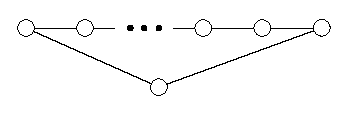
\includegraphics{table1_1(l)} & 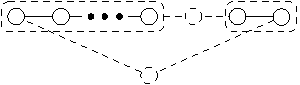
\includegraphics{table1_1(r)}
&  \\ \hline
$C_n$ & 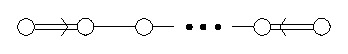
\includegraphics{table1_3(l)} & 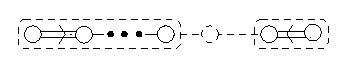
\includegraphics{table1_3(r)}
&  \\ \hline
$D_n$ & 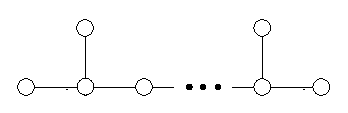
\includegraphics{table1_4(l)} & 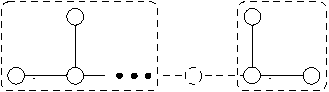
\includegraphics{table1_4(r)}
&  \\ \hline
\end{tabular}
}
\caption{Subalgebras $\af,\;\af_{\bot }$ for the classical series}
\end{table}


In the case of $B$ series the situation is different. The reason is that
here the subalgebra $\af_{\bot }$ may be larger than the one obtained
by elimination of the subdiagram of $\af$ and the adjacent nodes. The
subalgebras of the orthogonal pair,$\ \af$ and $\af_{\bot }$, must
not form a direct sum in $\frak{g}$ . It can be directly
checked that when $\frak{g}=B_{r}$ and $\af=B_{r_{\af}}$ the
orthogonal subalgebra is $\af_{\bot }=B_{r-r_{\af}}$. Consider the
injection $B_{r_{\af}}\rightarrow B_{r},\quad 1<r_{\af}<r$. By
eliminating the simple root $\alpha _{r_{\af}-1}=e_{r_{\af%
}-1}-e_{r_{\af}}$ one splits the extended Dynkin diagram of $B_{r}$
into the disjoint diagrams for $\af=B_{r_{\af}}$ and $D_{r-r_{%
\af}}$. But the system $\Delta _{\af_{\perp }}$ contains not only
the simple roots $\left\{ e_{1}-e_{2},e_{2}-e_{3},\ldots ,e_{r_{\af%
}-2}-e_{r_{\af}-1},e_{1}+e_{2}\right\} $ but also the root $e_{r_{\frak{%
a}}-1}$. Thus $\Delta _{\af_{\perp }}$ forms the subsystem of the type $%
B_{r-r_{\af}}$ and the orthogonal pair for the injection $B_{r_{\af%
}}\rightarrow B_{r}$ is $\left( B_{r_{\af}},B_{r-r_{\af}}\right) $%
. In the next Section a particular case of such orthogonal pair is
presented for the injection $B_{2}\rightarrow B_{4}$ (see Figure \ref
{fig:dynkin}).



The complete classification of regular subalgebras for affine Lie algebras
can be found in the recent paper \cite{1751-8121-41-36-365204}. From the complete
classification of maximal special subalgebras in classical Lie algebras \cite
{dynkin1952semisimple} we can deduce the following list of pairs of
orthogonal subalgebras $\af,\;\af_{\bot }$:
\begin{equation*}
\begin{array}{lll}
su(p)\oplus su(q) & \subset su(pq) &  \\
so(p)\oplus so(q) & \subset so(pq) &  \\
sp(2p)\oplus sp(2q) & \subset so(4pq) &  \\
sp(2p)\oplus so(q) & \subset sp(2pq) &  \\
so(p)\oplus so(q) & \subset so(p+q) & \mathrm{{for}\;p\;{and}\;q\;{odd}.}
\end{array}
\end{equation*}


\subsubsection{Algorithm for recursive computation of branching coefficients}

\label{sec:algorithm}

The recurrent relation (\ref{recurrent-relation}) allows us to formulate an
algorithm for recursive computation of branching coefficients. In this
algorithm there is no need to construct the module $L^{(\mu)}_{\frak{g}}$ or
any of the modules $L^{(\nu)}_{\af}$.

It contains the following steps:

\begin{enumerate}
\item  Construct the root system $\Delta _{\af}$ for the embedding $%
\af\rightarrow \frak{g}$.

\item  Select all positive roots $\alpha \in \Delta ^{+}$ orthogonal
to  $\af$, i.e. form the set $\Delta_{\afb }^{+}$.

\item  Construct the set $\Gamma _{\af\rightarrow \frak{g}}$. Relation
 (\ref{eq:6}) defines the sign function
 $s(\gamma)$ and the set $\Phi_{\af\subset \frak{g}}$ where the lowest weight
 $\gamma_0$ is to be subtracted to get the fan (\ref{fan-defined}):
 $\Gamma _{\af\rightarrow \frak{g}}=\left\{ \xi -\gamma _{0}|\xi \in \Phi _{%
\af\subset \frak{g}}\right\} \setminus \left\{ 0\right\}$.

\item  Construct the set $\widehat{\Psi ^{(\mu )}}=\left\{ w (\mu +\rho
)-\rho ;\;w \in W\right\} $ of singular weights for the $\frak{g}$%
-module $L^{(\mu )}$.

\item  Select the weights $\left\{ \mu _{\widetilde{\af_{\perp }}%
}\left( w\right) =\pi _{\widetilde{\af_{\perp }}}\left[ w(\mu +\rho
)-\rho \right] -\mathcal{D}_{\af_{\perp }}\in \overline{C_{\widetilde{%
\af_{\perp }}}}\right\} $. Since the set $\Delta_{\afb }^{+}$ is fixed
we can easily check wether the weight $\mu _{\widetilde{\af_{\perp }}%
}\left( w\right) $ belongs to the main Weyl chamber $\overline{C_{\widetilde{%
\af_{\perp }}}}$ (by computing its scalar product with the fundamental
weights of $\afb^{+}$).

\item  For the weights $\mu _{\widetilde{\af_{\perp }}}\left( w\right) $
calculate dimensions of the corresponding modules, $\mathrm{\dim }\left(
L_{\widetilde{\af_{\perp }}}^{\mu _{\widetilde{\af_{\perp }}%
}\left( u\right) }\right) $, using the Weyl dimension formula and construct
the singular element $\Psi ^{\left( \mu \right) }_{\left(  \af, \afb \right)}$.

\item  Calculate the anomalous branching coefficients using the
recurrent relation (\ref{recurrent-relation}) and select among them those
corresponding to the weights in the main Weyl
chamber $\overline{C_{\af}}$.
\end{enumerate}

We can speed up the algorithm by
one-time computation of the representatives of the conjugate classes $%
W/W_{\afb }$.

The next section contains examples illustrating the application of this
algorithm.

\subsection{Branching for finite dimensional Lie algebras}
\label{sec:finite-dimens-lie}

\subsubsection{Regular embedding of $A_1$ into $B_2$}
\label{sec:regul-embedd-a_1}

Consider the regular embedding $A_1\to B_2$. Simple roots $\alpha_1, \alpha_2$ of $B_2$
are presented as dashed vectors in Figure \ref{fig:B2_A1}. We denote the corresponding
Weyl reflections by $w_1, w_2$. The simple root $\beta = \alpha_1+2\alpha_2$ of $A_1$ is
grey.


\begin{figure}[p]
  \noindent\centering{
    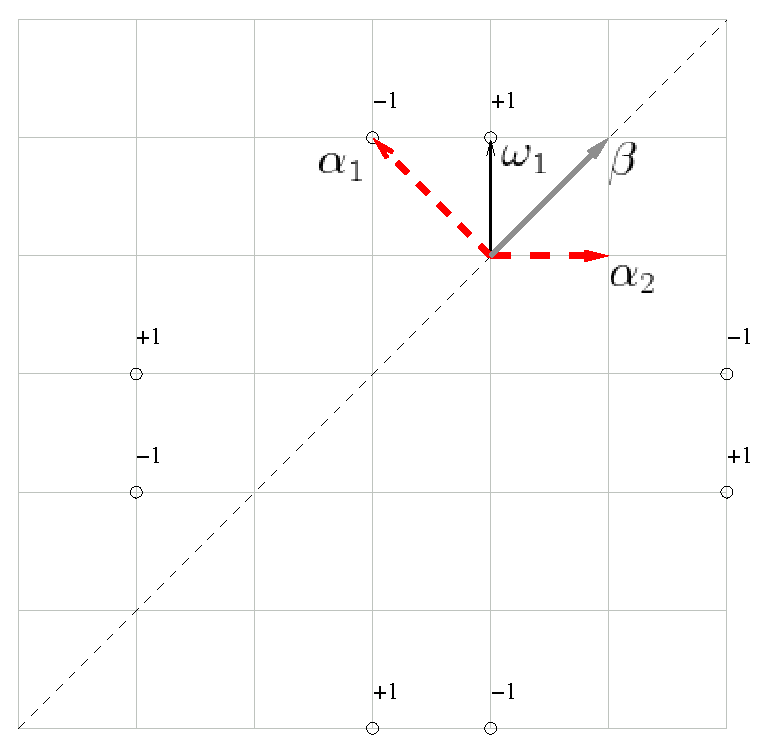
\includegraphics[width=80mm]{figure1}
  }
  \caption{Regular embedding of $A_1$ into $B_2$. Simple roots $\alpha_1, \alpha_2$ of $B_2$
  are presented as dashed vectors.
  The simple root $\beta = \alpha_1+2\alpha_2$ of $A_1$ is grey.
  The highest weight of the fundamental representation $L^{(1,0)=\omega_1}_{B_2}$ is black.
  The weights of the singular element $\Psi^{(\omega_1)}$ are marked by circles with
  superscripts indicating the corresponding determinants $\epsilon(w)$.}
  \label{fig:B2_A1}

%\end{figure}
%\begin{figure}[pb]
  \noindent\centering{
    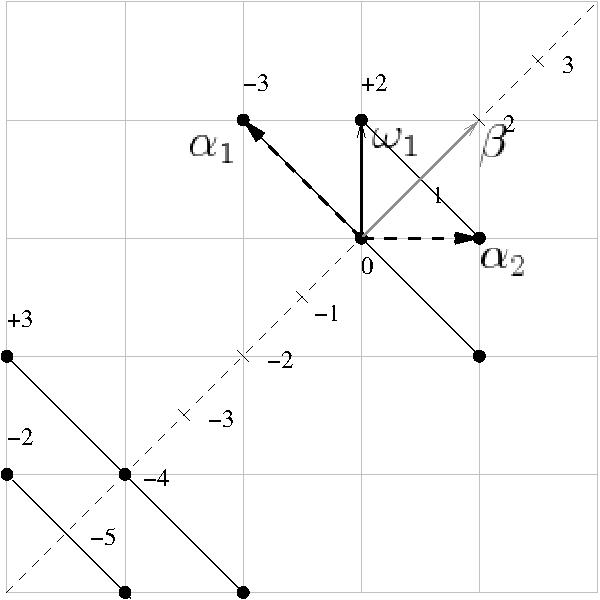
\includegraphics[width=80mm]{figure2}
  }
  \caption{Here in addition to the diagram presented above (Figure(\ref{fig:B2_A1}))
  the weights of $\left( \afb=A_1 \right)$-modules $L_{\af_{\perp }}^{\mu_{\af_{\perp }}\left( u\right) }$
  originating in the points $\pi _{\af}\left[ u(\mu +\rho )-\rho \right] $
are shown by dotted lines.
    The superscripts over the highest weights  $\mu_{\af_{\perp }}\left( u\right)$
    are now the products $\epsilon(u)\dim\left(L_{\af_{\perp }}^{\mu_{\af_{\perp }}\left( u\right) }\right)$.
    Coordinates along the root $\beta$ are counted in terms of the fundamental weight of $\af$. }
\label{fig:B2_A1_2}
\end{figure}


Let's perform the reduction of the fundamental representation $L^{(1,0)=\omega_1}_{B_2}$
($\omega_1$ -- the black vector in Figure \ref{fig:B2_A1}) according to the steps of the algorithm.
The root $\alpha_1$ is orthogonal to $\beta$,
so we have $\Delta_{\afb}^+ = \left\{ \alpha_1 \right\}$ (step (ii)).
According to Definition \ref{fan-definition}
the fan $\Gamma_{A_1\to B_2}$ (step (iii)) consists of two weights:
\begin{equation*}
  \label{eq:22}
  \Gamma_{A_1\to B_2}=\left\{ (1;2),\; (2;-1) \right\},
\end{equation*}
where the second component is the value of the sign function $s(\gamma)$.
Singular weights  $\left\{ w (\omega_1 +\rho)-\rho ;\;w \in W\right\}$ (step (iv))
are indicated by circles with the superscript $\epsilon\left( w \right)$.
The space $U$ is the factor $W/W_{\afb}$ where $W_{\afb}=\left\{e,w_1\right\}$.
This means that singular weights located above the $\beta$-line
belong to the Weyl chamber $\overline{C_{\widetilde{\af_{\perp }}}}$.
According to formula (\ref{defect-perp}) we have $\mathcal{D}_{\af_{\perp }}=0$ and
$\hf_{\perp }=0$, thus $\left\{ \mu _{\af_{\perp }}\left( w\right)
=\pi _{\af_{\perp }}\left[ w(\mu +\rho)-\rho \right]\right\}$.
We obtain four highest weights for $\af_{\perp }$-modules. In terms of
$\af_{\perp }$-fundamental weight $\frac{1}{2} \alpha_1$ these highest weights
$\left\{ \mu _{\af_{\perp }}\left( u\right)
=\pi _{\af_{\perp }}\left[ u(\mu +\rho)-\rho \right]| u \in U \right\}$
 are
$\left\{ \left( 1\right) \left( 2\right) \left( 2\right) \left( 1\right) \right\}$ (step v).
In Figure (\ref{fig:B2_A1_2}) the corresponding weight diagrams
$\left\{ \mathcal{N}_{\af_{\perp }}^{\mu _{\af_{\perp }}\left( u\right) }\right\} $
are attached to the set of $\af$-weights
$\left\{ \mu _{\af}\left( u\right)\right\} =\left\{\pi _{\af}\left[ u(\mu +\rho )-\rho \right]\right\}
=\left\{ \left( 1\right) \left( 0\right) \left( -4\right) \left( -5\right) \right\}$.
In fact we do not need the
weight diagrams but only the dimensions of modules
$L_{\af_{\perp }}^{\mu_{\af_{\perp }}\left( u\right) }$ multiplied by
$\epsilon \left( u\right) $ (step vi). Obtained values are to be attributed to the points
$\left\{ \left( 1\right) \left( 0\right) \left( -4\right) \left( -5\right) \right\}$
in $P_{\af}$. The singular element $\Psi ^{\left( \mu \right) }_{\left(  \af, \afb \right)}$
has the set of weights with anomalous multiplicities:
\begin{equation}
  \label{eq:25}
  \left\{(1;2),\; (0;-3),\; (-4;3),\; (-5;-2)\right\}.
\end{equation}

Applying formula (\ref{recurrent-relation}) with the fan
$\Gamma_{A_1\to B_2}$ to the set (\ref{eq:25}) (step vii)
we get zeros for the weights
greater than the highest anomalous vector $(1;2)$
and $k^{(1,0)}_1=2$ for the vector $(1;2)$ itself.
For the anomalous weight (0;-3) on the boundary of $\bar{C}^{(0)}_{\af}$ the recurrent relation gives
\begin{equation*}
  \label{eq:23}
  k^{(1,0)}_{0}=-1\cdot k^{(1,0)}_2 +2\cdot k^{(1,0)}_1 - 3\cdot \delta_{0,0} = 1,
\end{equation*}
the branching is completed: $L_{B_2\downarrow A_1}^{\omega_1}=
2L_{A_1}^{\omega_{\left(A_1\right)} }
\bigoplus
L_{A_1}^{2\omega_{\left(A_1\right)} }$.

\subsubsection{Embedding $B_2$ into $B_4$}
\label{sec:someth-high-dimens}
Consider the regular embedding $B_2 \rightarrow B_4$.
The corresponding Dynkin diagrams are presented in the Figure \ref{fig:dynkin}.
\begin{figure}[h]
  \centering
  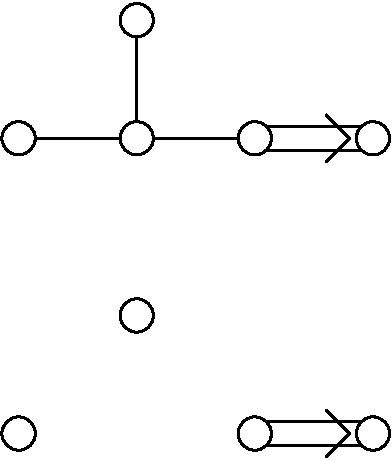
\includegraphics[width=100mm]{figure3}
  \caption{The regular embedding $B_2 \rightarrow B_4$ described by dropping the node from the Dynkin diagram.
  Remember that here $\afb$ is equal to $B_2$ while the diagram
  shows only $A_1\oplus A_1$ (see Subsection \ref{sect-embeddings}).}
  \label{fig:dynkin}
\end{figure}

\begin{figure}[pt]
  \centering
    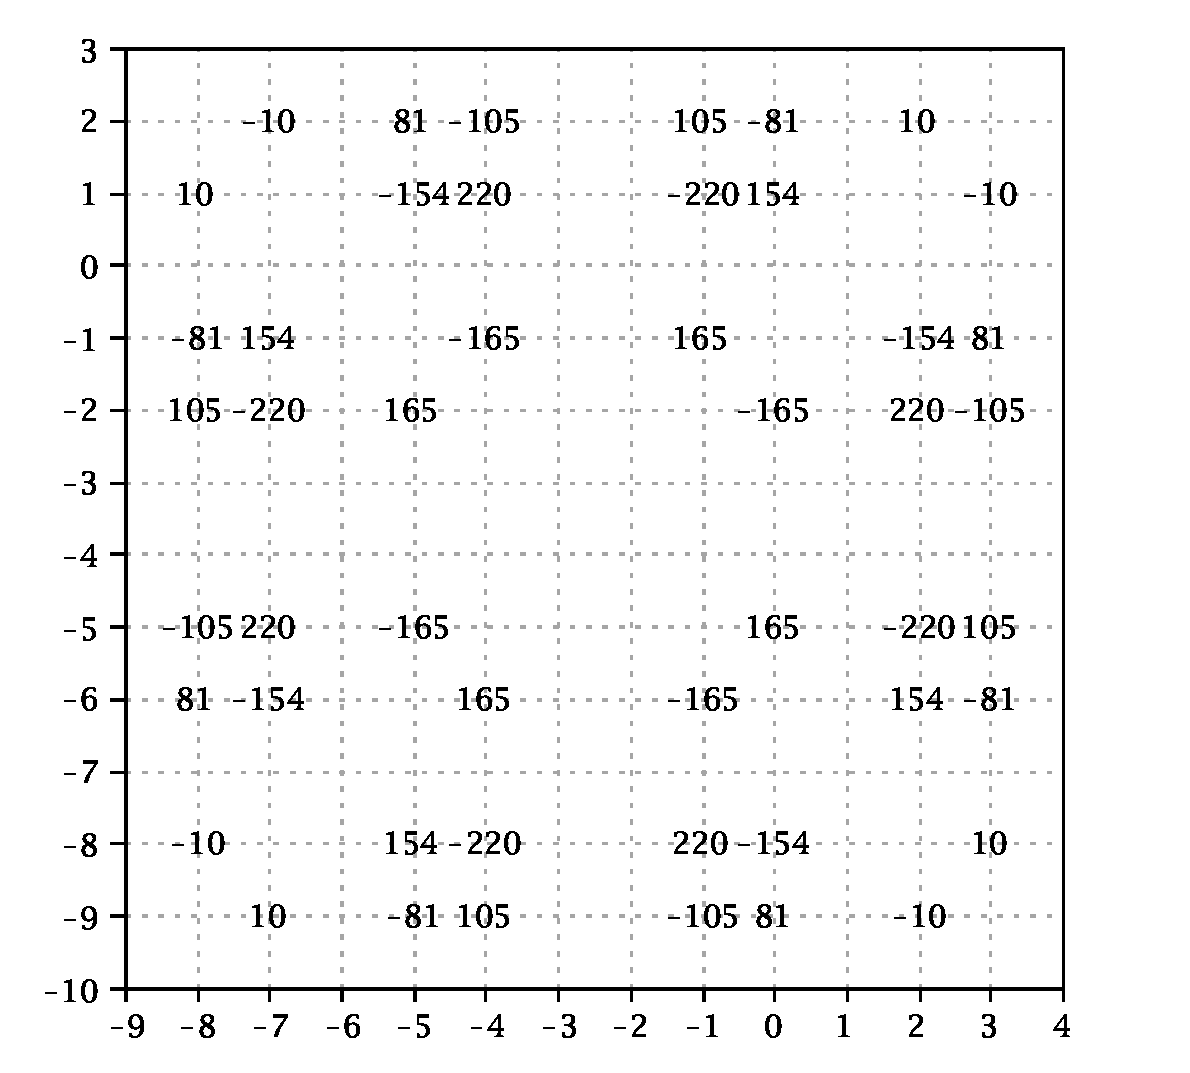
\includegraphics[width=100mm,height=90mm]{figure4}
  \caption{The singular element $e^{\gamma_0}\Psi ^{\left( \mu \right) }_{\left(  \af, \afb \right)}$
  displayed in the weight subspace $P_{\af}$ for $\af=B_2$ with the basis $\left\{e_3,e_4\right\}$.
  We see the projected singular weights $\left\{\pi _{\af}\left[ u(\mu +\rho )-\rho \right] +\gamma_0 | u \in U \right\}$
  shifted by $\gamma_0$ and supplied by multipliers
  $\epsilon(u)\dim\left(L_{\af_{\perp }}^{\mu_{\af_{\perp }}\left( u\right) }\right)$.}
  \label{fig:B4B2anom}

%\end{figure}
%
%\begin{figure}[pb]
  \centering
  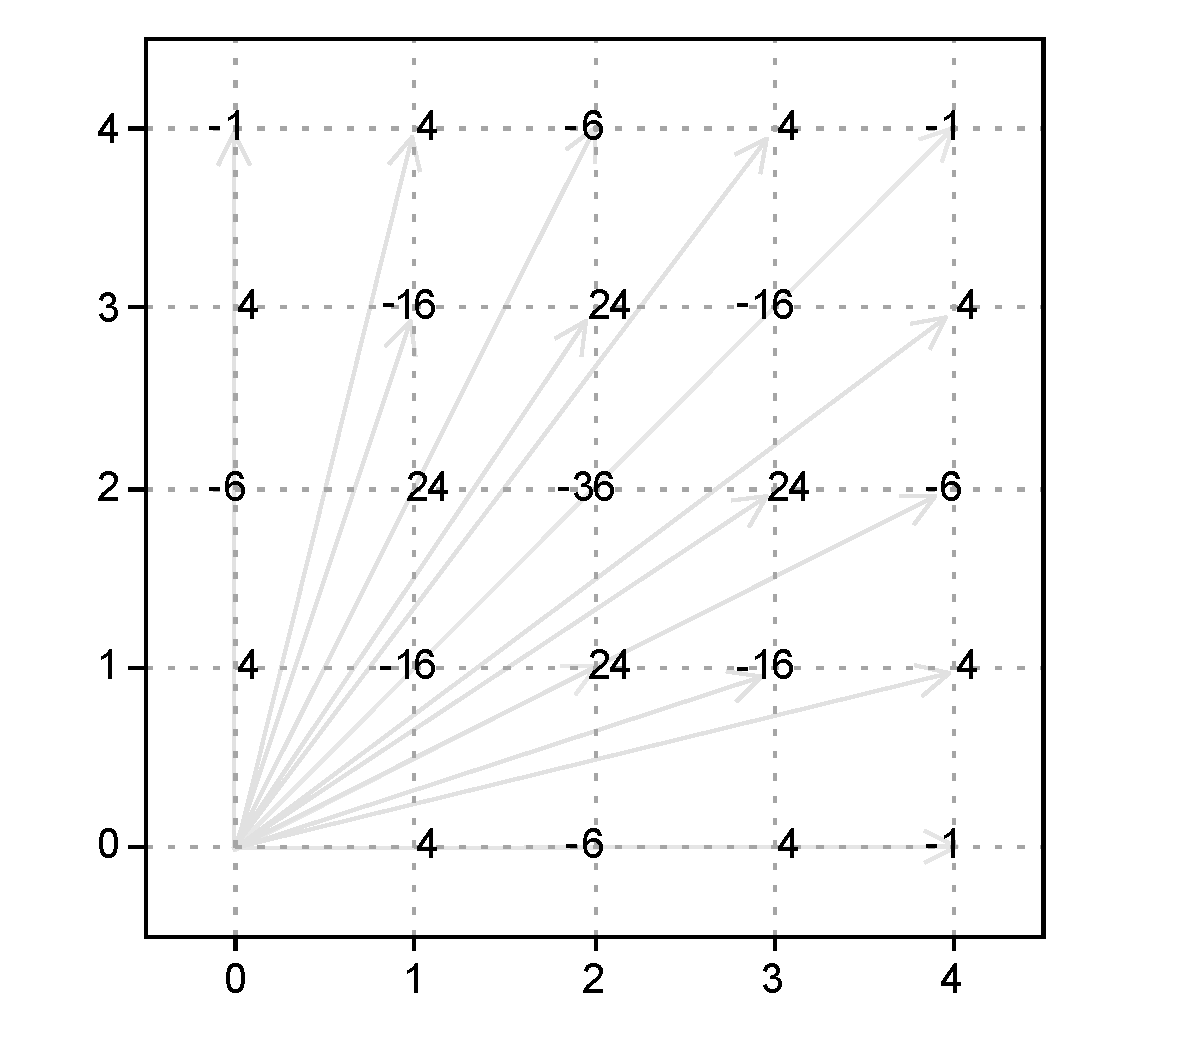
\includegraphics[height=80mm]{figure5}
  \caption{The fan $\Gamma$ for $B_2\rightarrow B_4$ with values of $s(\gamma+\gamma_0)$ attributed to each $\gamma \in \Gamma$.}
  \label{fig:B4B2Fan}
\end{figure}

In the orthonormal basis $\left\{e_1,\dots,e_4\right\}$ simple roots and positive roots of $B_4$ are
\begin{eqnarray*}
  \label{eq:19}
  S_{B_4}= \{e_1 - e_2,\; e_2 - e_3,\; e_3 - e_4,\; e_4\},\\[2mm]
 \Delta^+_{B_4}=\left\{ (e_1 - e_2,\; e_2 - e_3,\; e_3 - e_4,\; e_4,\; e_1 - e_3,\; e_2 - e_4,\; e_3 + e_4,\; e_3,\; e_1 - e_4,\;\right.\\
 \left. e_2 + e_4,\; e_2,\; e_1 + e_4,\; e_2 + e_3,\; e_1,\; e_1 + e_3,\; e_1 + e_2\right\}
\end{eqnarray*}
The subalgebra $\af=B_2$ is fixed by the simple roots
\begin{equation*}
  \label{eq:26}
 S_{B_2}=\{e_3-e_4,e_4\}.
\end{equation*}
Its orthogonal counterpart $\afb=B_2$ has
\begin{eqnarray*}
  \label{eq:27}
  S_{\afb}=\{e_1-e_2,e_2\},\\
 \Delta^{+}_{\afb}= \left\{e_1-e_2,e_1+e_2,e_1,e_2\right\}.
\end{eqnarray*}
As far as the set $\Delta^+_{B_4} \setminus  \Delta^{+}_{\afb}$ is fixed the injection
fan $\Gamma_{B_2 \to B_4}$ can be constructed using Definition \ref{fan-definition}.
As far as for this injection $s\left( \gamma_0\right)=-1$ in the recursion formula we need only the factor
 $s\left(\gamma + \gamma_0\right)$.
The result is presented in Figure \ref{fig:B4B2Fan}.


Consider the $B_4$-module $L^{\mu}$ with the highest weight $\mu=2e_1 + 2 e_2 + e_3 + e_4$; \,
$\mathrm{dim}(L^{\left[0,1,0,2\right]})=2772$.
Here the defect is nontrivial, $\mathcal{D}_{\af_{\perp }}=-2\left( e_1 + e_2 \right)$,
while $\hf_{\bot}=0$. Among the singular weights there are
48 vectors with the property $\left\{ \mu _{\af_{\perp }%
}\left( u\right) =\pi _{\af_{\perp }}\left[ u(\mu +\rho
)-\rho \right] -\mathcal{D}_{\af_{\perp }}\in \overline{C_{\af_{\perp }}}\right\} $.
The set $U=\left\{ u \right\}$ is thus fixed.
Compute the dimensions of the corresponding $\afb$-modules with the highest weights
$ \mu _{\af_{\perp }}\left( u\right)$ (using the Weyl dimension formula) and multiply them
by $\epsilon\left( u \right)$. The result is the singular element
$\Psi ^{\left( \mu \right) }_{\left(  \af, \afb \right)}$ shown in Figure \ref{fig:B4B2anom}.

Now one can place the fan $\Gamma$ (see Figure \ref{fig:B4B2Fan}) in the highest of the weights
presented in Figure \ref{fig:B4B2anom} and start the recursive determination of the branching coefficients
(using relation (\ref{recurrent-relation})):
\begin{eqnarray*}
  \label{eq:24}
  \pi_{\af} \left(ch L^{\left[0,1,0,2\right]}_{B_4}\right) = 6 \; ch L^{\left[0,0\right]}_{B_2}+ 60
  \; ch L_{B_2}^{\left[0,2\right]}+ 30 \; ch L_{B_2}^{\left[1,0\right]}+ 19 \; ch L_{B_2}^{\left[2,0\right]}+\\
  40 \; ch L_{B_2}^{\left[1,2\right]}+ 10 \; ch L_{B_2}^{\left[0,4\right]}.
\end{eqnarray*}
%\newpage
\subsection{Applications to conformal field theory}
\label{sec:phys-appl}

\subsubsection{Conformal embeddings}
\label{sec:conformal-embeddings}

Branching coefficients for an embedding of affine Lie algebra into
affine Lie algebra can be used to construct modular invariant
partition functions for Wess-Zumino-Novikov-Witten models in conformal field theory
(\cite{difrancesco1997cft}, \cite{Walton:1999xc}, \cite{walton1989conformal}, \cite{schellekens1986conformal}).
In these models current algebras are affine Lie algebras.

The modular invariant partition function is crucial for the conformal theory to be valid
on the torus and higher genus Riemann surfaces. It is important for the applications of
CFT to string theory and to critical phenomena description.

The simplest modular-invariant partition function has the diagonal form:
\begin{equation}
  \label{eq:34}
   Z(\tau)=\sum_{ \mu\in P^{+}_{\mathfrak{g}}} \chi_{\mu}(\tau)\bar \chi_{\mu}(\bar \tau)
\end{equation}
Here the sum is over the set of highest weights for integrable modules in a WZW-model
and $\chi_{\mu}(\tau)$ are the normalized characters (see \cite{difrancesco1997cft}) of these modules.

To construct nondiagonal modular invariants is not an easy problem,
although for some models the complete classification of modular invariants is known \cite{1994hepthGannon,1995JMPGannon}.

Consider the Wess-Zumino-Witten model with the affine Lie algebra $\af$.
Nondiagonal modular invariants for this model can be constructed from the diagonal
invariant if there exists an affine algebra $\mathfrak{g}$ such that $\af\subset\mathfrak{g}$.
Then we can replace the characters of the $\mathfrak{g}$-modules in the diagonal
modular invariant partition function (\ref{eq:34})
by the decompositions
\begin{equation*}
  \label{eq:32}
\sum_{\nu \in P^{+}_{\af}}b^{(\mu)}_{\nu} \chi_{\nu}
\end{equation*}
containing normalized characters $\chi_{\nu}$ of the corresponding $\af$-modules.
Thus we obtain a nondiagonal modular-invariant  partition function for the theory with
the current algebra $\af$,
\begin{equation}
  \label{eq:36}
   Z_{\af}(\tau)=\sum_{ \nu,\lambda\in P^{+}_{\af}} \chi_{\nu}(\tau)M_{\nu\lambda}\bar \chi_{\lambda}(\bar \tau).
\end{equation}

The effective reduction procedure is crucial for this construction.
The embedding is required to preserve the conformal invariance.
Let $X^{\alpha_j}_{-n_j}$ and $\tilde{X}^{\alpha'_j}_{-n_j}$ be the lowering generators for
$\mathfrak{g}$ and for $\af\subset\mathfrak{g}$ correspondingly.
Let $\pi_{\af}$ be the projection operator of
$\pi_{\af}:\mathfrak{g}\longrightarrow \af$.
In the theory attributed to $\mathfrak{g}$ with the vacuum $\left|\lambda\right>$
the states can be described as
\begin{equation*}
  \label{eq:109}
  X^{\alpha_1}_{-n_1}X^{\alpha_2}_{-n_2}\dots\left|\lambda\right>\quad n_1\geq n_2\geq \dots>0.
\end{equation*}
And for the sub-algebra $\af$ the corresponding states are
\begin{equation*}
  \label{eq:110}
  \tilde{X}^{\alpha'_1}_{-n_1}\tilde{X}^{\alpha'_2}_{-n_2}\dots\left|\pi_{\af}(\lambda)\right>.
\end{equation*}
The $\mathfrak{g}$-invariance of the vacuum entails its $\af$-invariance,
but this is not the case for the energy-momentum tensor. So the energy-momentum tensor of the larger theory
should contain only the generators $\tilde{X}$. Then the relation
\begin{equation}
  \label{eq:2}
  T_{\mathfrak{g}}(z)=T_{\af}(z)
\end{equation}
leads to the equality of central charges
\begin{equation*}
  \label{eq:33}
  c(\mathfrak{g})=c(\af)
\end{equation*}
and to the relation
\begin{equation}
  \label{eq:111}
  \frac{k\;\mathrm{dim}\,\mathfrak{g}}{k+g}=\frac{x_e k\; \mathrm{dim}\,\af}{x_ek+a}.
\end{equation}
Here $x_e$ is the so called "embedding index":
$x_e=\frac{\left|\pi_{\mathfrak{a}} \Theta\right|^2}{\left|\Theta_{\mathfrak{a}}\right|^2}$
with $\Theta$, $\Theta_{\mathfrak{a}}$ being the highest roots of
$\mathfrak{g}$ and $\mathfrak{a}$
while $g$  and $a$ are the  corresponding dual Coxeter numbers.

It can be demonstrated that solutions of equation (\ref{eq:111}) exist only
for the level $k=1$ \cite{difrancesco1997cft}.

The complete classification of conformal embeddings is given in \cite{schellekens1986conformal}.

The relation (\ref{eq:111}) and the asymptotics of the branching functions can be used
to prove the finite reducibility theorem \cite{kac1988modular}.
It states that for a conformal embedding  $\af\longrightarrow\mathfrak{g}$
only finite number of branching coefficients have nonzero values.

\begin{mynote} The orthogonal subalgebra $\afb$ is always trivial
for conformal embeddings $\af\longrightarrow \mathfrak{g}$.
\begin{proof}
Consider the modes expansion of the energy-momentum tensor
\begin{equation*}
\label{eq:47}
  T(z)=\frac{1}{2(k+h^v)}\sum_n z^{-n-1}L_n.
\end{equation*}
The modes $L_n$ are constructed as combinations of normally-ordered products of $\gf$-algebra generators,
\begin{equation*}
\label{eq:48}
  L_n=\frac{1}{2(k+h^v)}\sum_{\alpha}\sum_m:X^{\alpha}_m X^{\alpha}_{n-m}: \; .
\end{equation*}
In case of a conformal embedding energy-momentum tensors $T_{\mathfrak{g}}(z)$ and $T_{\af}(z)$ are
equal (see (\ref{eq:2})).

In these combinations we are to substitute  $\af$-generators in terms of $\mathfrak{g}$-generators
and obtain the energy-momentum tensor $T_{\mathfrak{g}}$.
But if the set of generators attributed to $\Delta_{\afb}$ is not empty this is not possible,
since $T_{\mathfrak{g}}$ contains generators $X^{\alpha}_n$ for $\alpha\in \Delta_{\afb}$.
\end{proof}
\end{mynote}



\subsubsection{Special embedding $\hat{A}_1\rightarrow\hat{A}_2$.}
\label{sec:spec-embedd-hata_1s}

Consider the case where both $\gf$ and $\af$ are affine Lie algebras:
$\hat{A}_1 \rightarrow \hat{A}_2$ and the injection is the affine extension of the
special injection $A_1 \rightarrow A_2$ with the embedding index $x_e=4$.
As far as $\gf$-modules to be considered are of level one,
the necessary $\af$-modules will be of level $\tilde{k}=kx_e=4$.

There exist three level one fundamental weights of $\hat{A}_2$.
It is easy to see that the set $\Delta_{ \afb }$ is empty and the subalgebra $\afb=0$.
Then ${\cal D}_{\afb}=0$, $\hf_{\perp}$ is one-dimensional abelian subalgebra and
the dimension of $\tilde\afb=\afb\oplus \hf_{\perp}$ is also 1.
It is convenient to choose the classical root for $\hat{A}_1$ to be
$\beta=\frac{1}{2}(\alpha_1+\alpha_2)$.

Using Definition (\ref{fan-definition})  we construct the fan $\Gamma_{\hat A_1\to\hat A_2}$.
In this case $\gamma_0 =0$ and its sign $s\left( 0 \right)=-1$ thus we are to use the
sign function $s(\gamma)$ (see Figure \ref{fig:AffineA2A1Fan}).


\begin{figure}[h!bt]
  \centering
  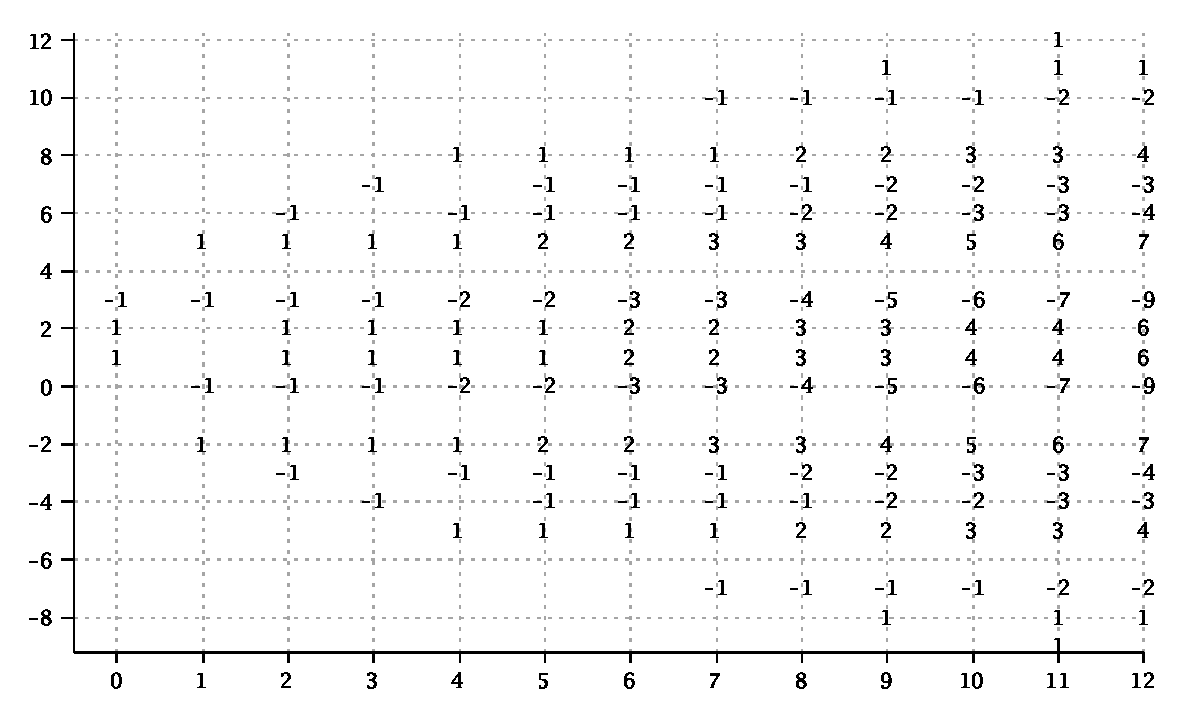
\includegraphics[width=125mm]{figure6}

  \caption{The fan $\Gamma_{\hat{A_1}\rightarrow \hat{A_2}}$ for $\hat{A_1}\rightarrow \hat{A_2}$
  in the basis $\left\{\beta,\delta \right\}$. Notice that $\gamma_0 =0$, so values of $s(\gamma)$
  are prescribed to the weights $\gamma\in \Gamma_{\hat{A_1}\rightarrow \hat{A_2}}$}
  \label{fig:AffineA2A1Fan}
\end{figure}

Consider the module $L^{\omega_0=(0,0;1;0)}$. Here we use the (finite part; level; grade)
presentation of the highest weight and the finite part
coordinates are the Dynkin indices (see section(\ref{sec:notation})).

The set $\widehat{\Psi^{(\omega_0)}}$  is displayed in Figure
\ref{fig:affine_A2_anom_point} up to the sixth grade.

\begin{figure}[h!tb]
  \hspace*{-1.5cm}
  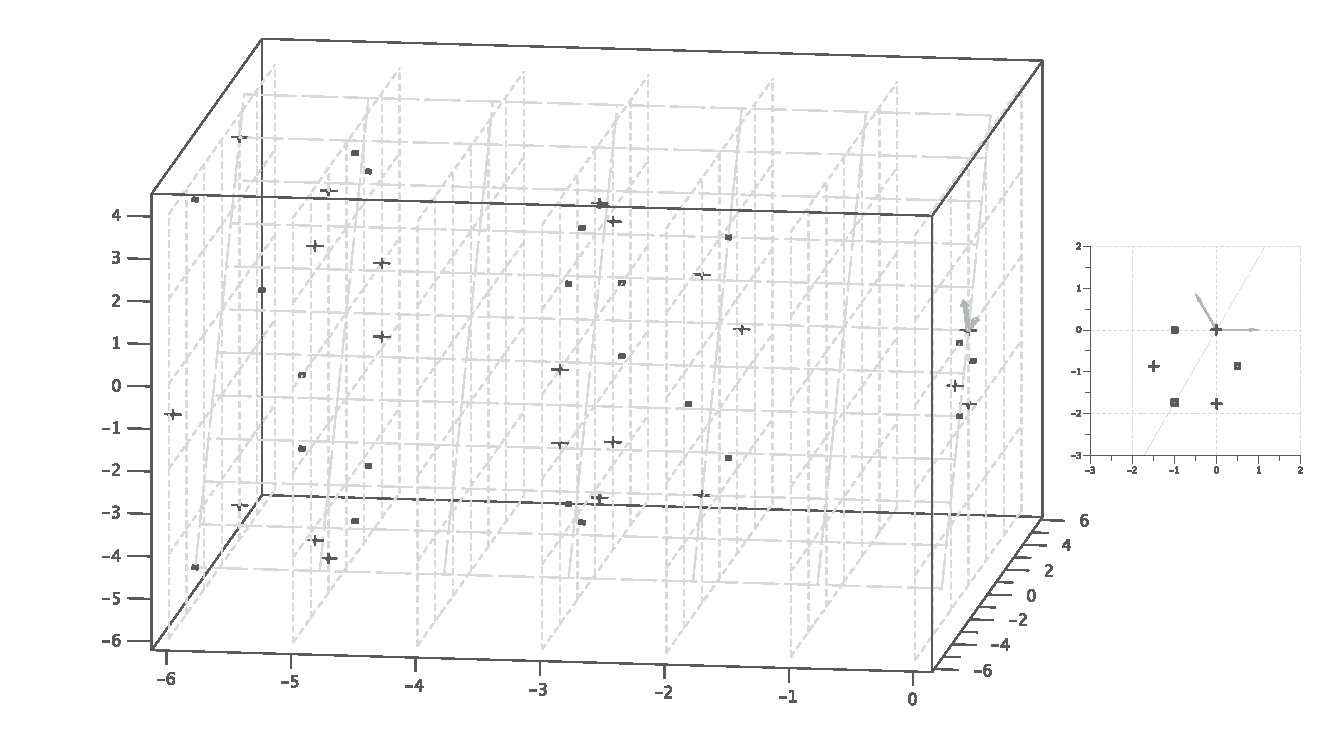
\includegraphics[width=180mm]{figure7}
  \caption{Singular weights of the module $L_{\hat{A_2}}^{\omega_0}=L^{(0,0;1;0)}_{\hat{A_2}}$.
   The classical (grade zero) cross-section of the diagram is shown separately
   in the right part of the figure.
  We use the orthogonal basis with the unit vector equal to $\alpha_1$.
  The weights $w (\omega_0+\rho)-\rho$ are marked by crosses when $\epsilon(w)=1$ and
by box when $\epsilon(w)=-1$. Simple roots of the classical subalgebra $A_2$ are
grey and the grey diagonal plane corresponds to the Cartan subalgebra of
the embedded algebra $\hat{A}_1$.}
  \label{fig:affine_A2_anom_point}
\end{figure}

The next step is  to project the anomalous weights to $P_{\hat A_1}$.
The result is the element $\Psi ^{\left( \omega_0 \right) }_{\left(  \hat A_1\, , \, \afb=0 \right)}$
presented in Figure \ref{fig:AffineA2_A1_anom_proj} up to the twelfth grade.
\begin{figure}[h!tb]
  \centering
  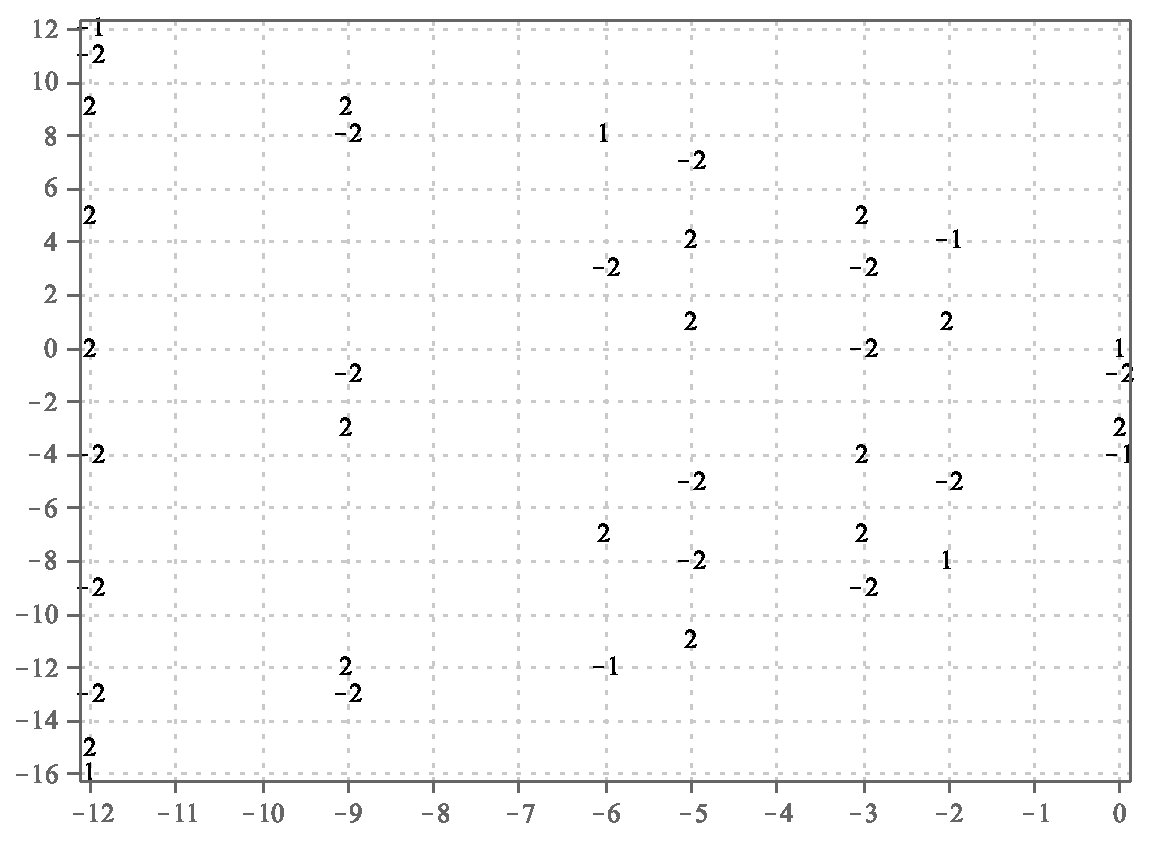
\includegraphics[width=130mm]{figure8}
  \caption{The singular element $\Psi ^{\left( \omega_0 \right) }_{\left(  \hat A_1\, , \, \afb=0 \right)}$
  displayed in $P_{\hat A_1}$
  with the basis $\left\{\beta,\delta \right\}$.}
  \label{fig:AffineA2_A1_anom_proj}
\end{figure}


Using the recurrent relation (\ref{recurrent-relation}) with the fan
$\Gamma_{\hat{A_1}\rightarrow \hat{A_2}}$ and the singular weights in
$\Psi ^{\left( \omega_0 \right) }_{\left(  \hat A_1\, , \, \afb=0 \right)}$
we get the anomalous branching coefficients presented
in Figure \ref{fig:AffineA2_A1_branching}.
\begin{figure}[h!tb]
  \centering
  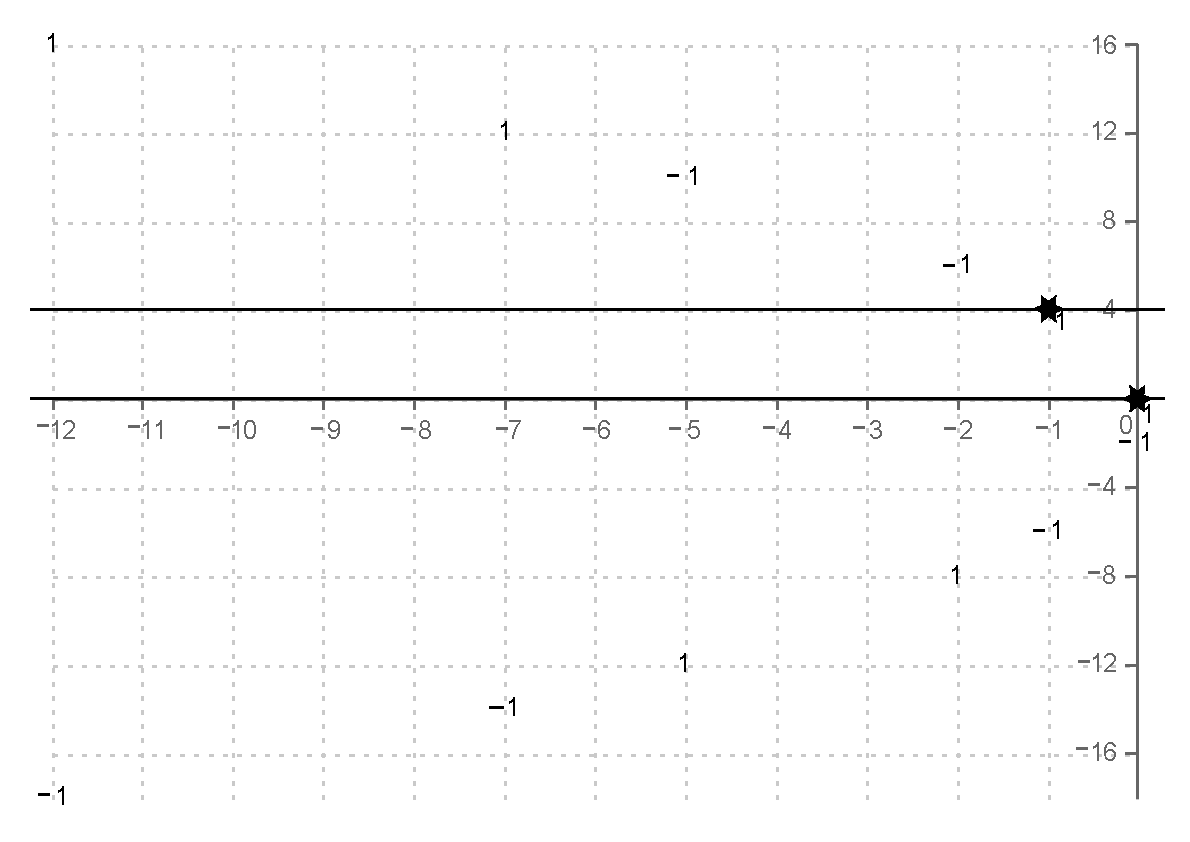
\includegraphics[width=130mm]{figure9}
  \caption{Anomalous branching coefficients for $\hat{A_1}\subset \hat{A_2}$. The boundaries
  of the main Weyl chamber $\bar{C}_{\hat{A}_1}$
 are indicated by black lines. Two anomalous highest weights located
 in the main Weyl chamber are marked by stars.
 Both have multiplicity 1, so the branching coefficients for them are equal 1.}
  \label{fig:AffineA2_A1_branching}
\end{figure}
Inside the Weyl chamber $\bar{C}_{\hat{A}_1}$
(its boundaries are indicated in Figure \ref{fig:AffineA2_A1_branching})
there are only two nonzero anomalous weights and both have multiplicity 1.
These are the highest weights of $\af$-submodules and the multiplicities are their branching
coefficients. Thus we get the decomposition
\begin{equation*}
  \label{eq:43}
  L^{(0,0;1;0)}_{\hat{A_2}\downarrow \hat{A_1}}= L_{\hat{A_1}}^{(0;4;0)}\oplus L_{\hat{A_1}}^{(4;4;0)}.
\end{equation*}
Notice that the finite reducibility theorem holds.

The same fan $\Gamma_{\hat{A_1}\rightarrow \hat{A_2}}$ can be used for any other highest weight
module $L^{\mu}_{\hat{A_2}}$. In particular for irreducible modules of level one  we get the trivial
branching:
\begin{equation*}
  \label{eq:44}
   L^{(1,0;1;0)}_{\hat{A_2}\downarrow \hat{A_1}}= L_{\hat{A_1}}^{(2;4;0)},\\
   L^{(0,1;1;0)}_{\hat{A_2}\downarrow \hat{A_1}}= L_{\hat{A_1}}^{(2;4;0)}.
\end{equation*}

Using these results the modular-invariant partition function is easily found,
\begin{equation*}
  \label{eq:45}
  Z=\left|\chi_{(4;4;0)}+\chi_{(0;4;0)}\right|^2+2\chi_{(2;4;0)}^2.
\end{equation*}

\subsubsection{Coset models}
\label{sec:coset-models}

Coset models \cite{Goddard198588} tightly connected with the gauged WZW-models are actively studied
in string theory, especially in string models on anti-de-Sitter space
\cite{Maldacena:2000hw,Maldacena:2000kv,Maldacena:2001km,Maldacena:2001ky,Aharony:1999ti}.
The characters in coset models are proportional to branching functions,
\begin{equation}
  \label{eq:31}
  \chi^{(\mu)}_{\nu}(\tau)=e^{2\pi i \tau (m_{\mu}-m_{\nu})} b^{(\mu)}_{\nu}(\tau),
\end{equation}
with
\begin{equation*}
  \label{eq:46}
  m_{\mu}=\frac{\left|\mu+\rho\right|^2}{2(k+g)}-\frac{\left|\rho\right|^2}{2g}.
\end{equation*}
The problem of branching functions construction in the coset models was considered
in  \cite{Dunbar:1992gh}, \cite{Hwang:1994yr}, \cite{lu1994branching}.

Let us return to our example \ref{sec:regul-embedd-a_1} and consider the affine extension of the injection
$A_1 \rightarrow B_2$.
Since this embedding is regular and $x_e=1$, the subalgebra modules and the initial module are of the same level.
The set  of positive roots with zero projection
on the root space of the subalgebra $\hat{A_1}$ is the same as in the finite-dimensional case:
$\Delta^{+}_{\afb}=\left\{ \alpha_1 \right\}$ and $\afb=A_1$. It is easy to see that here $\hf_{\perp}$
is trivial and ${\cal D}_{\afb}=0$.

Using Definition (\ref{fan-definition}) we obtain the fan
$\Gamma_{\hat{A_1} \longrightarrow  \hat{B_2} }$.
Notice that here the lowest weight  $\gamma_0$ of the fan  is zero and $s\left( \gamma_0 \right)=-1$.
Values of the sign function $s(\gamma)$ for
$ \gamma \in \Gamma_{\hat{A_1} \longrightarrow  \hat{B_2} }$ are presented in Figure \ref{fig:AffineB2A1Fan}.
We restricted the computation to the twelfth grade.
\begin{figure}[h!bt]
  \centering
  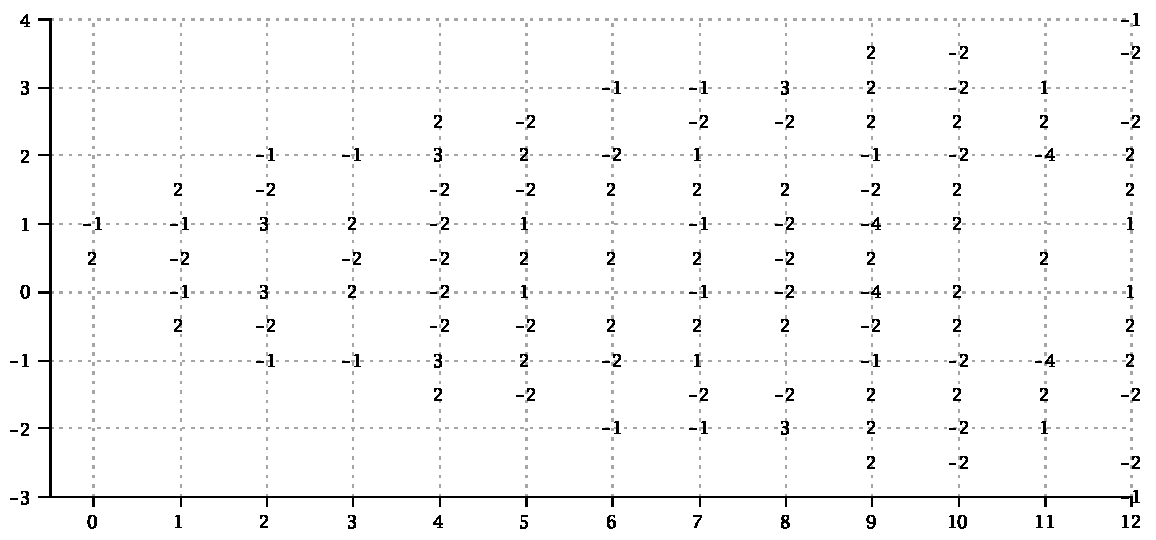
\includegraphics[width=135mm]{figure10}
  \caption{The fan $\Gamma_{\hat{A_1}\rightarrow \hat{B_2}}$
  for $\hat{A_1}\rightarrow \hat{B_2}$ in the basis $\left\{\beta,\delta \right\}$. Values of  $s(\gamma)$ are shown for the
  weights $\gamma\in \Gamma_{\hat{A_1}\rightarrow \hat{B_2}}$}
  \label{fig:AffineB2A1Fan}
\end{figure}


Consider the level one module $L^{\left( 1,0;1;0 \right)}_{\hat{B_2}}$  with the highest weight $\omega_1=(1,0;1;0)$,
where the finite part coordinates are in the orthogonal basis $e_1,e_2$.
The set of anomalous weights for this module up to the sixth grade is presented in Figure \ref{fig:affine_B2_anom_point}.

\begin{figure}[h!tb]
%  \hspace*{-2cm}
  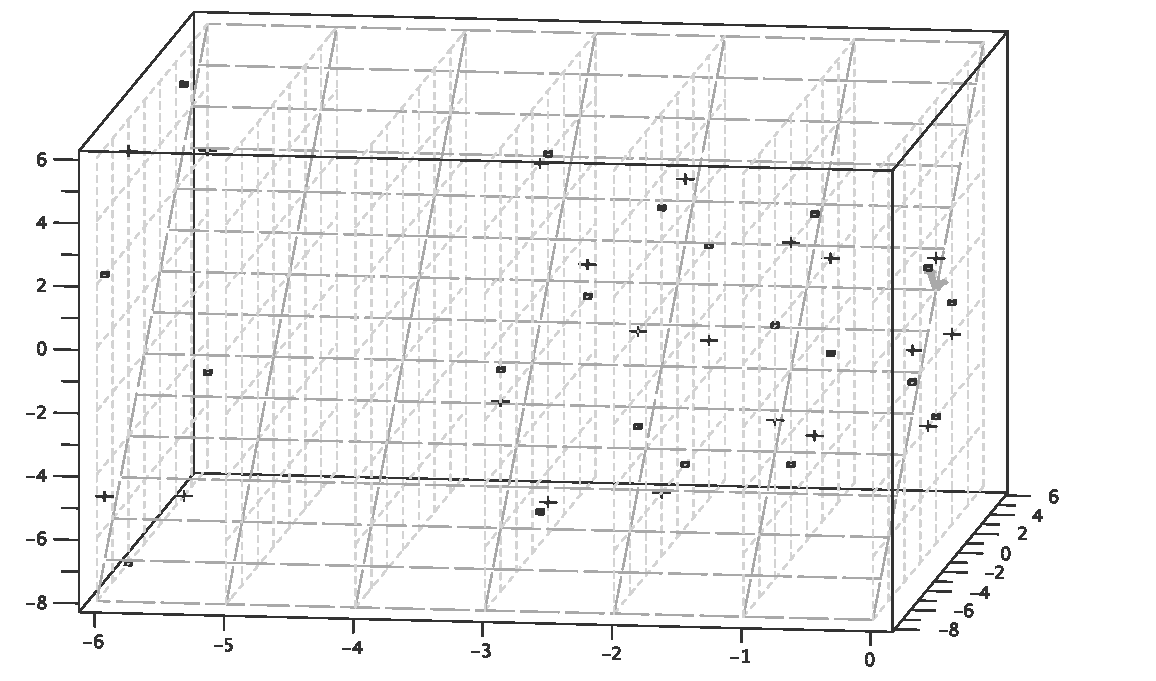
\includegraphics[width=140mm]{figure11}
  \caption{Singular weights for $L^{(1,0;1;0)}_{\hat B_2 }$. The standard basis $\{e_1,e_2\}$ is used for the classical cross-section.
  The weights in the zero grade are the same as in Figure \ref{fig:B2_A1}.
  The weights $w (\omega_1+\rho)-\rho$ are marked by crosses if $\epsilon(w)=1$ and by boxes for $\epsilon(w)=-1$.
Simple roots of the classical subalgebra $B_2$ are grey and grey diagonal plane corresponds to the Cartan subalgebra
of the embedded algebra $\hat{A}_1$.}
  \label{fig:affine_B2_anom_point}
\end{figure}

According to the recursive algorithm \ref{sec:algorithm} we project these anomalous weights to
$P_{\hat{A_1}}$ and find the dimensions of the corresponding
$\afb$-modules $L^{\pi_{\afb}(w(\mu+\rho))-\rho_{\afb}}_{\afb}$.
In the grade zero this projection gives exactly the set
$\Psi ^{\left( \mu \right) }_{\left(  A_1, A_1 \right)}$ for the embedding of
the classical Lie algebra $A_1\rightarrow B_2$. To see this compare Figure \ref{fig:B2_A1}
with Figure \ref{fig:AffineB2_A1_anom_proj}
where the singular element $\Psi ^{\left( \mu \right) }_{\left(  \widehat{A_1}, A_1 \right)}$
for the affine embedding $\hat{A_1}$ is presented up to the twelfth grade.
\begin{figure}[h!tb]
  \centering
  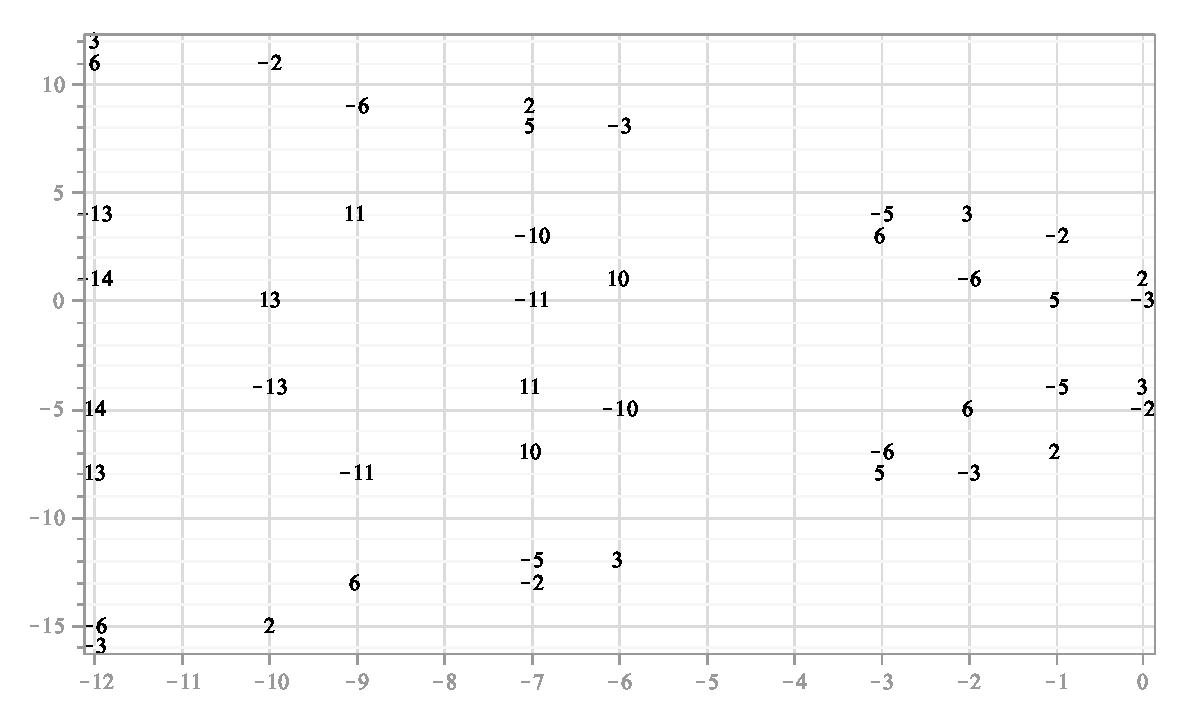
\includegraphics[width=120mm]{figure12}
  \caption{Singular element $\Psi ^{\left( \omega_1 \right) }_{\left(  \widehat{A_1}, A_1 \right)}$
  in the basis $\{\beta,\delta\}$. Dimensions of the corresponding $\afb=A_1$-modules
  with the signs $\epsilon(u)$ are indicated.}
  \label{fig:AffineB2_A1_anom_proj}
\end{figure}

\begin{figure}[h!bt]
  \centering
  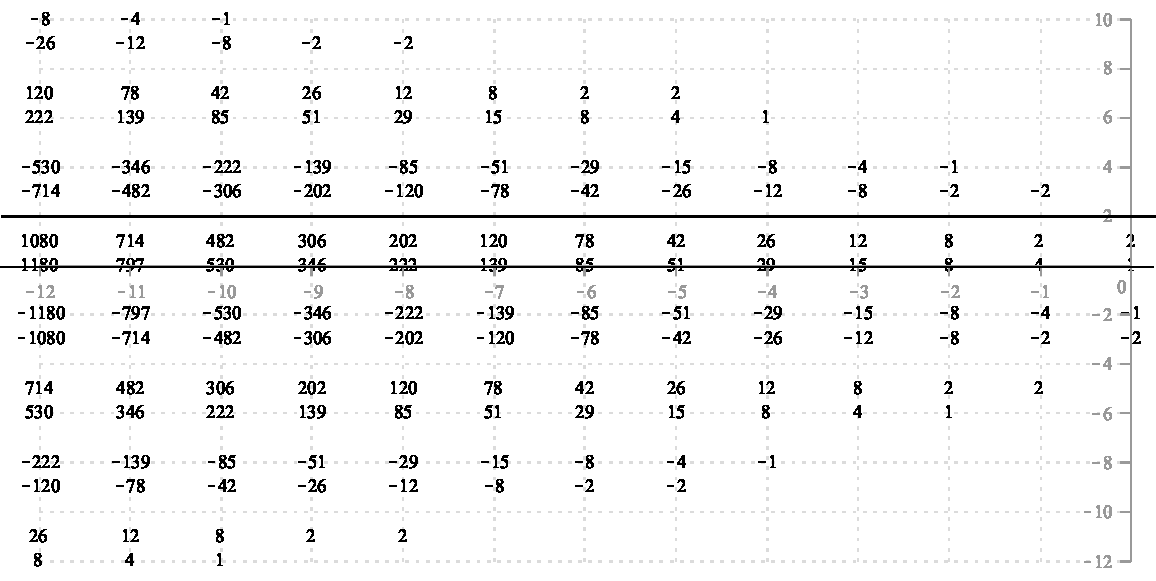
\includegraphics[width=120mm]{figure13}
  \caption{Anomalous branching coefficients for $\hat{A_1}\rightarrow \hat{B_2}$. The basis $\{\beta,\delta\}$ is used.
 Boundaries  of the main Weyl chamber $\bar{C}_{\hat{A}_1}$
 are indicated by black lines. Anomalous branching coefficients
 inside the main Weyl chamber are equal to branching coefficients of the embedding $\hat{A_1}\rightarrow \hat{B_2}$.}
  \label{fig:AffineB2_A1_branching}
\end{figure}

Multiplicities of the highest weights inside the  Weyl chamber
$\bar{C}^{\left( 0 \right)}_{\hat{A_1}}$
define the following branching coefficients (up to the twelfth grade),
\begin{eqnarray*}
  \label{eq:28}
  L^{\omega_1}_{\hat{B_2}\downarrow \hat{A_1}}
  &=&2 L_{\hat{A_1}}^{\omega_1}\oplus 1 L_{\hat{A_1}}^{\omega_0}\oplus 4 L_{\hat{A_1}}^{\omega_0-\delta}\oplus\\
    &&2 L_{\hat{A_1}}^{\omega_1-\delta}\oplus 8 L_{\hat{A_1}}^{\omega_0-2\delta}\oplus
    8 L_{\hat{A_1}}^{\omega_1-2\delta}\oplus 15 L_{\hat{A_1}}^{\omega_0-3\delta}\oplus\\
    &&12 L_{\hat{A_1}}^{\omega_1-3\delta}\oplus 26 L_{\hat{A_1}}^{\omega_1-4\delta}\oplus
    29 L_{\hat{A_1}}^{\omega_0-4\delta}\oplus 51 L_{\hat{A_1}}^{\omega_0-5\delta}\oplus\\
    &&42 L_{\hat{A_1}}^{\omega_1-5\delta}\oplus 78 L_{\hat{A_1}}^{\omega_1-6\delta}\oplus
    85 L_{\hat{A_1}}^{\omega_0-6\delta}\oplus 120 L_{\hat{A_1}}^{\omega_1-7\delta}\oplus\\
    &&139 L_{\hat{A_1}}^{\omega_0-7\delta}\oplus 202 L_{\hat{A_1}}^{\omega_1-8\delta}\oplus
    222 L_{\hat{A_1}}^{\omega_0-8\delta}\oplus 306 L_{\hat{A_1}}^{\omega_1-9\delta}\oplus\\
    &&346 L_{\hat{A_1}}^{\omega_0-9\delta}\oplus 530 L_{\hat{A_1}}^{\omega_0-10\delta}\oplus
    482 L_{\hat{A_1}}^{\omega_1-10\delta}\oplus 714 L_{\hat{A_1}}^{\omega_1-11\delta}\oplus\\
    &&797 L_{\hat{A_1}}^{\omega_0-11\delta}\oplus 1080 L_{\hat{A_1}}^{\omega_1-12\delta}\oplus
    1180 L_{\hat{A_1}}^{\omega_0-12\delta}\oplus \dots
\end{eqnarray*}
This result can be presented as the set of branching functions:
\begin{eqnarray*}
  \label{eq:29}
  \begin{array}{cc}
    b^{(\omega_1)}_{0}= & 1 + 4\,q^{1}+ 8\,q^{2}+ 15\,q^{3}+ 29\,q^{4}+ 51\,q^{5}+ 85\,q^{6}+ 139\,q^{7}+\\
     &222\,q^{8}+ 346\,q^{9}+ 530\,q^{10}+ 797\,q^{11}+ 1180\,q^{12}+\dots\\
  \end{array}\\
  \begin{array}{cc}
    b^{(\omega_1)}_{1}= &2+2\,q^{1}+8\,q^{2}+12\,q^{3}+26\,q^{4}+42\,q^{5}+78\,q^{6}+120\,q^{7}+\\
    & 202\,q^{8}+306\,q^{9}+482\,q^{10}+714\,q^{11}+1080\,q^{12}+\dots
  \end{array}
\end{eqnarray*}
Here $q=\exp (2\pi i \tau)$ and the lower index enumerates the branching functions according
to their highest weights in $P^+_{\hat{A_1}}$.
These are the fundamental weights $\omega_0=\lambda_0=(0,1,0),\; \omega_1=\alpha/2=(1,1,0)$.

Now we can return to (\ref{eq:31}),
\begin{equation*}
  \label{eq:35}
  \begin{array}{cc}
    \chi^{(\omega_1)}_{1}(q)= & q^{\frac{7}{12}}\left( 2+2\,q^{1}+8\,q^{2}+12\,q^{3}+26\,q^{4}+42\,q^{5}+78\,q^{6}+120\,q^{7}+\right. \\
    & \left. 202\,q^{8}+306\,q^{9}+482\,q^{10}+714\,q^{11}+1080\,q^{12}+\dots \right),\\
    \chi^{(\omega_1)}_{0}(q) = & q^{\frac{5}{6}}\left(1 + 4\,q^{1}+ 8\,q^{2}+ 15\,q^{3}+ 29\,q^{4}+ 51\,q^{5}+ 85\,q^{6}+ 139\,q^{7}+\right. \\
    &\left. 222\,q^{8}+ 346\,q^{9}+ 530\,q^{10}+ 797\,q^{11}+ 1180\,q^{12}+\dots\right),
  \end{array}
\end{equation*}
and finally obtain expansions for the $B_2/A_1$-coset characters.


\subsection{Conclusion}
\label{sec:conclusion}
We have demonstrated that the injection fan technique can be used to deal with arbitrary
reductive subalgebras (maximal as well as  nonmaximal).
It was shown that the branching problem for $\af \subset \gf$  is tightly connected with
the properties of the orthogonal partner $ \af_{\perp
} $ of $\af$. The subalgebra $\afb$ corresponds to the subset
$\Delta^{+}_{\afb}$ of positive roots in $\Delta_{\mathfrak{g}}^{+}$ that trivialize
the Cartan subalgebra $\hf_{\afb}$.
Both the injection fan and the sets of singular weights for
highest weight $\gf$-modules depend substantially on the structure of $\afb$ and its submodules.
For the fan $\Gamma_{\af\rightarrow \gf}$ this dependence is almost obvious:
in the element $\Phi_{\af\rightarrow \gf}$ the factors corresponding to the roots
of $\Delta^{+}_{\afb}$ are eliminated.
The transformation in the set of projected singular weights is more interesting.
We have found out that in the new singular element
$\Psi ^{\left( \mu \right) }_{\left(  \af, \afb \right)}$ the coefficients depend on
the $\afb$-submodules (their highest weights $\mu _{\widetilde{\af_{\perp }}}\left( u\right)$
are fixed by the injection and by the weights of the initial
element $\Psi^{\mu}$).
Fortunately no more information on $L^{\mu _{\widetilde{\af_{\perp }}}\left( u\right)}
_{\left\{ \afb \right\}}$-submodules is necessary than their dimensions.
In the new singular element $\Psi ^{\left( \mu \right) }_{\left(  \af, \afb \right)}$
weight multiplicities are equal to dimensions
$\dim\left(L^{\mu _{\widetilde{\af_{\perp }}}\left( u\right)}_{\left\{ \afb \right\}}\right)$
of the corresponding $\afb$-modules
multiplied by the values $\epsilon (u)$. As a result
the highest weights of $\af$-submodules and their
multiplicities are subject to the set of linear equations (\ref{eq:17}).
These properties are valid for any reductive subalgebra $\af\rightarrow \gf$ and
the set can be redressed to the form of recurrent relations to be solved step by step.

The efficiency of the obtained algorithm was illustrated in various examples.
In particular we considered the construction of modular-invariant partition functions
in the framework of conformal embedding method and the coset construction in rational conformal field theory.
This construction is useful in the study of WZW-models
emerging in the context of the AdS/CFT correspondence \cite{Maldacena:2000hw,Maldacena:2000kv,Maldacena:2001km}.

Further amelioration of the algorithm can be achieved by using
the folded fan technique \cite{il2010folded}. It must be mentioned that even in the case
of string functions the explicit solution of the corresponding recurrent relations is
a difficult problem (see \cite{il2010folded} for details). Nevertheless we hope that by
developing the procedure of folding one could get explicit solutions
for at least some of branching functions and the corresponding coset characters.




\section{БГГ-резольвента}
\label{sec:bgg}
Категория О.
Резольвента Бернштейна-Гельфанда-Гельфанда для представлений аффинных алгебр Ли. Параболические модули и их связь с подалгебрами и ветвлением.


\begin{abstract}
Рекуррентные соотношения для коэффициентов ветвления основываются на определенном разложении сингулярного элемента. Мы показываем, что такое разложение может использоваться для построения параболических модулей Верма и получения обобщенных формул Вейля-Верма для характеров. Также мы демонстрируем, что коэффициенты ветвления определяют обобщенную резольвенту Бернштейна-Гельфанда-Гельфанда. 
\end{abstract}

\subsection{Введение}

\label{sec:introduction}
Свойства ветвления (аффинных) алгебр Ли важны для приложений в квантовой теории поля (смотри, например, модели конформной теории поля \cite{difrancesco1997cft},\cite{coquereaux2008conformal}). В данной работе мы показываем, что ветвление для произвольной редуктивной подалгебры связано с БГГ резольвентой и демонстрирует свойства резольвенты в категории $\mathcal{O}^{p}$ \cite{lepowsky1977generalization} (параболического обобщения категории $\mathcal{O}$ \cite{bernstein1976category}).

Резольвента для неприводимых модулей в терминах бесконечномерных модулей важна для теории интегрируемых спиновых цепочек \cite{derk1008}. В подходе  $\mathcal{Q}$-оператора Бакстера \cite{derk09} общие трансфер-матрицы, соответствующие (обобщенным) модулям Верма, факторизуются в произведение операторов Бакстера. Резольвента позволяет вычислить трансфер-матрицы для конечномерных вспомогательных пространств.

Чтобы продемонстрировать связь БГГ резольвенты с ветвлением мы используем рекурсивный подход, представленный в работе \cite
{2010arXiv1007.0318L} (аналогичный подход для максимальных вложений использовался в работе \cite{ilyin812pbc}). Мы рассматриваем подалгебру $\af \hookrightarrow \gf$ вместе с $\afb$ -- ``ортогональным партнером'' $\af$ по отношению к форме Киллинга, а также подалгебру $\widetilde{\afb}:=\afb\oplus \frak{h}_{\perp }$, где $\frak{h}=\frak{\frak{h}_{\af}}\oplus
\frak{h}_{\afb}\oplus \frak{h}_{\perp }$. Для любой редуктивной подалгебры $\af$ алгебра $\afb\hookrightarrow \gf$ регулярна и редуктивна. Для интегрируемого модуля старшего веса $%
L^{\left(\mu \right) }$ и ортогональной подалгебры  $\af_{\bot }$ мы рассматриваем сингулярный элемент $\Psi ^{\left( \mu \right) }$ (числитель в формуле Вейля для характеров $ch\left( L^{\mu }\right) =\frac{\Psi ^{\left(
\mu \right) }}{\Psi ^{\left( 0\right) }}$, см., например,  \cite
{humphreys1997introduction}) и знаменатель Вейля $\Psi _{\af_{\bot
  }}^{\left( 0\right) }$ для ортогонального партнера. В работе показано, что элемент  $\Psi _{\gf%
}^{\left( \mu \right) }$ может быть разложен в комбинацию числителей Вейля $\Psi _{\af_{\bot }}^{\left( \nu \right) }$, где $\nu \in P_{%
\mathfrak{a}_{\bot}}^{+}$. Это разложение дает возможность построить множество модулей старшего веса $L_{\afb}%
^{\mu _{\afb}}$. В том случае, если вложение\ $\af%
_{\bot }\hookrightarrow \gf$ \ удовлетворяет ``стандартным параболическим'' условиям, эти модули порождают параболические модули Верма $M_{\left(
\afb \hookrightarrow \gf\right) }^{\mu _{%
\afb}}$, так что исходный характер $ch\left(
L^{\mu }\right) $ в итоге раскладывается в знакопеременную сумму таких модулей. С другой стороны, если параболическое условие нарушено, конструкция сохраняется и порождает разложение по отношению к набору обобщенных модулей Верма  $M_{\left( \widetilde{\frak{b}_{\perp }},\gf\right) }^{\mu _{%
\widetilde{\afb}}}$, где $%
\widetilde{\frak{b}_{\perp }}$ уже не является подалгеброй в $\gf$, а оказывается сжатием $\widetilde{\afb}$.

Некоторые общие свойства предложенного разложения формулируются в терминах  формального элемента $\Gamma _{\af\rightarrow \gf}$, называемого ``веером вложения''. Использование этого инструмента позволило сформулировать простой и явный алгоритм для вычисления правил ветвления, подходящий для произвольной (максимальной или не максимальной) подалгебры в аффинной алгебре Ли \cite{2010arXiv1007.0318L}.

Возможные обобщения полученных результатов обсуждаются в Разделе \ref{sec:conclusions}.


\subsection{Ортогональная подалгебра и сингулярные элементы}

\label{sec:recurr-form-branch}

В этом разделе мы покажем, как рекуррентный подход к проблеме ветвления естественным образом приводит к представлению формального характера $\frak{g}$-модуля в виде комбинации характеров, соответствующих параболическим (обобщенным) модулям Верма. Рассмотрим редуктивную алгебру Ли  $\frak{g}$ и ее редуктивную подалгебру $\frak{a}\subset \frak{g}$.
Пусть  $L^{\mu} $ -- интегрируемый модуль старшего веса алгебры  $\frak{g}$, $\mu \in P^{+}$.  Будем считать  $L^{\mu}$ вполне приводимым по отношению к подалгебре $\frak{a}$,
\begin{equation*}
L_{\frak{g}\downarrow \frak{a}}^{\mu }=\bigoplus\limits_{\nu \in P_{\frak{a}%
}^{+}}b_{\nu }^{\left( \mu \right) }L_{\frak{a}}^{\nu }.
\end{equation*}
Это разложение может быть записано в терминах формальных характеров с использованием оператора проекции  $\pi _{\frak{a}}$ (на весовое пространство $\frak{h_{a}}^{\ast }$):
\begin{equation}
\pi _{\frak{a}}ch\left( L^{\mu }\right) =\sum_{\nu \in P_{\frak{a}%
}^{+}}b_{\nu }^{(\mu )}ch\left( L_{\frak{a}}^{\nu }\right) .
\label{branching1}
\end{equation}
Для модуля  $L^{\mu }$ существует БГГ резольвента (см. \cite
{bernstein1976category,bernstein1975differential,bernstein1971structure} и
\cite{humphreys2008representations}). Все члены фильтрующей последовательности представляются суммами модулей Верма со старшими весами $\nu$, сильно связанными с $\mu$:
\begin{equation*}
\left\{ \nu \right\} =\left\{ w\left( \mu +\rho \right) -\rho |w\in
W\right\} .
\end{equation*}

\subsubsection{Ортогональная подалгебра}

Пусть  $\frak{h}_{\frak{a}}$ -- подалгебра Картана в  $\mathfrak{g}$. Для  $\mathfrak{a}\hookrightarrow \frak{g}$ введем ``ортогонального партнера''  $\mathfrak{a}_{\bot }\hookrightarrow \frak{g}$.

Рассмотрим корневое подпространство  $\frak{h}_{\perp \frak{a}}^{\ast }$, ортогональное к $\frak{a}$,
\begin{equation*}
\frak{h}_{\perp \frak{a}}^{\ast }:=\left\{ \eta \in \frak{h}^{\ast }|\forall
h\in \frak{h}_{\frak{a}};\eta \left( h\right) =0\right\} ,
\end{equation*}
и корни  $\frak{g}$ (соответственно, положительные корни),  ортогональные к $\frak{a}$,
\begin{eqnarray}
\Delta _{\frak{a}_{\perp }} &:&=\left\{ \beta \in \Delta _{\frak{g}}|\forall
h\in \frak{h}_{\frak{a}};\beta \left( h\right) =0\right\} ,
\label{delta a ort} \\
\Delta _{\frak{a}_{\perp }}^{+} &:&=\left\{ \beta ^{+}\in \Delta _{\frak{g}%
}^{+}|\forall h\in \frak{h}_{\frak{a}};\beta ^{+}\left( h\right) =0\right\} .
\notag
\end{eqnarray}
Обозначим символом  $W_{\frak{a}_{\perp }}$ подгруппу  $W$, порожденную отражениями  $w_{\beta }$ с корнями  $\beta \in \Delta_{\frak{a}_{\perp}}^{+}$. Корневая подсистема  $\Delta _{\frak{a}_{\perp }}$ определяет подалгебру  $\frak{a}_{\perp }$, имеющую подалгебру Картана $\frak{h}_{\frak{a}_{\perp }}$. Пусть
\begin{equation*}
\frak{h}_{\perp }^{\ast }:=\left\{ \eta \in \frak{h}_{\perp \frak{a}}^{\ast
}|\forall h\in \frak{h}_{\frak{a}\oplus \frak{a}_{\perp }};\eta \left(
h\right) =0\right\};
\end{equation*}
выделим в  $\frak{g}$  подалгебры
\begin{eqnarray}
\widetilde{\frak{a}_{\perp }} :=\frak{a}_{\perp }\oplus \frak{h}_{\perp },
\qquad
\widetilde{\frak{a}} :=\frak{a}\oplus \frak{h}_{\perp }.
\end{eqnarray}
Заметим, что  $\mathfrak{a} \oplus \mathfrak{a}_{\bot}$ в общем случае не является подалгеброй в $\mathfrak{g}$.

Для подалгебр Картана имеет место разложение
\begin{equation}
\frak{h}=\frak{\frak{h}_{\frak{a}}}\oplus \frak{h}_{\frak{a}_{\perp }}\oplus
\frak{h}_{\perp }=\frak{\frak{h}_{\widetilde{\frak{a}}}}\oplus \frak{h}_{%
\frak{a}_{\perp }}=\frak{\frak{h}_{\widetilde{\frak{a}_{\perp }}}}\oplus
\frak{h}_{\frak{a}}.
\end{equation}
Рассмотрим векторы Вейля  $\rho _{\frak{a}}$ и $\rho _{\frak{a}_{\perp}} $, соответствующие  $\frak{a}$ и $\frak{a}_{\perp }$.
Введем так называемые ``дефекты'' вложения  $\mathcal{D}_{\frak{a}}$ и $\mathcal{D}_{\frak{a}_{\perp }}$:
\begin{equation}
\mathcal{D}_{\frak{a}}:=\rho _{\frak{a}}-\pi _{\frak{a}}\rho , \qquad
\mathcal{D}_{\frak{a}_{\perp }}:=\rho _{\frak{a}_{\perp }}-\pi _{\frak{a}%
_{\perp }}\rho .  \label{defect ort}
\end{equation}
Для  $\mu \in P^{+}$ рассмотрим связанные веса  $\left\{\left( w(\mu +\rho )-\rho \right) |w\in W\right\} $ и их проекции на $h_{\frak{a}_{\perp }}^{\ast }$, дополнительно сдвинутые на вектор дефекта $-\mathcal{D}_{\frak{a}_{\perp }}$:
\begin{equation*}
\mu _{\frak{a}_{\perp }}\left( w\right) :=\pi _{\frak{a}_{\perp }}\left[
w(\mu +\rho )-\rho \right] -\mathcal{D}_{\frak{a}_{\perp }},\quad w\in W.
\end{equation*}

Среди весов  $\left\{ \mu _{\frak{a}_{\perp
}}\left( w\right) |w\in W\right\} $ всегда можно выбрать те, которые попадают в фундаментальную камеру $\overline{C_{\frak{a}_{\perp }}}$. Пусть $U$ -- множество представителей $u$ классов  $W/W_{\frak{a}_{\perp }}$, таких что
\begin{equation}
U:=\left\{ u\in W|\quad \mu _{\frak{a}_{\perp }}\left( u\right) \in
\overline{C_{\frak{a}_{\perp }}}\right\} \quad .  \label{U-def}
\end{equation}
Тогда можно выделить подмножества:
\begin{equation}
\mu _{\widetilde{\mathfrak{a}}}\left( u\right) :=\pi _{\widetilde{%
\mathfrak{a}}}\left[ u(\mu +\rho )-\rho \right] +\mathcal{D}_{\frak{a}%
_{\perp }},\quad u\in U,  \label{mu-a}
\end{equation}
и
\begin{equation}
\mu _{\frak{a}_{\perp }}\left( u\right) :=\pi _{\frak{a}_{\perp }}\left[
u(\mu +\rho )-\rho \right] -\mathcal{D}_{\frak{a}_{\perp }},\quad u\in U.
\label{mu-a-tilda}
\end{equation}

Заметим, что подалгебра  $\mathfrak{a}_{\bot}$ по определению регулярна, так как она построена на подмножестве корней алгебры $\mathfrak{g}$.

Для интересующих нас модулей формула Вейля-Каца для  $\mathrm{ch}\left( L^{\mu }\right) $ может быть записана через сингулярные элементы \cite{humphreys1997introduction},
\begin{equation*}
\Psi ^{\left( \mu \right) }:=\sum\limits_{w\in W}\epsilon (w)e^{w(\mu +\rho
)-\rho },
\end{equation*}
а именно:
\begin{equation}
\mathrm{ch}\left( L^{\mu }\right) =\frac{\Psi ^{\left( \mu \right) }}{\Psi
^{\left( 0\right) }}=\frac{\Psi ^{\left( \mu \right) }}{R}.
\label{Weyl-Kac2}
\end{equation}
То же верно и для подмодулей $\mathrm{ch}\left( L_{\frak{a}}^{\nu
}\right) $ в формуле (\ref{branching1})
\begin{equation*}
\mathrm{ch}\left( L_{\frak{a}}^{\nu }\right) =\frac{\Psi _{\frak{a}}^{\left(
\nu \right) }}{\Psi _{\frak{a}}^{\left( 0\right) }}=\frac{\Psi _{\frak{a}%
}^{\left( \nu \right) }}{R_{\frak{a}}},
\end{equation*}
где
\begin{equation*}
\Psi _{\frak{a}}^{\left( \nu \right) }:=\sum\limits_{w\in W_{\frak{a}%
}}\epsilon (w)e^{w(\nu +\rho _{_{\frak{a}}})-\rho _{_{\frak{a}}}}.
\end{equation*}
Применяя формулу  (\ref{Weyl-Kac2}) к правилу ветвления  (\ref{branching1}) мы получаем соотношение, связывающее сингулярные элементы $\Psi ^{\left( \mu
\right) }$ и $\Psi _{\frak{a}}^{\left( \nu \right) }$ :
\begin{eqnarray}
\pi _{\frak{a}}\left( \frac{\sum_{w \in W}\epsilon (w )e^{w (\mu +\rho
)-\rho }}{\prod_{\alpha \in \Delta ^{+}}(1-e^{-\alpha })^{\mathrm{mult}%
(\alpha )}}\right) &=&\sum_{\nu \in P_{\frak{a}}^{+}}b_{\nu }^{(\mu )}\frac{%
\sum_{w \in W_{\frak{a}}}\epsilon (w )e^{w (\nu +\rho _{\frak{a}})-\rho _{%
\frak{a}}}}{\prod_{\beta \in \Delta _{\frak{a}}^{+}}(1-e^{-\beta })^{\mathrm{%
mult}_{\frak{a}}(\beta )}},  \notag  \label{eq:4} \\
\pi _{\frak{a}}\left( \frac{\Psi ^{\left( \mu \right) }}{R}\right)
&=&\sum_{\nu \in P_{\frak{a}}^{+}}b_{\nu }^{(\mu )}\frac{\Psi _{\frak{a}%
}^{\left( \nu \right) }}{R_{\frak{a}}}.
\end{eqnarray}

\subsubsection{Разложение сингулярного элемента.}

\label{subsec:decomp-sing-element}

Теперь мы выполним разложение сингулярного элемента  $\Psi ^{\left(\mu \right) }$ на сингулярные элементы модулей ортогонального партнера:

\begin{lemma}

Пусть  $\frak{a}_{\bot }$ -- ортогональный партнер редуктивной подалгебры  $\frak{a}\hookrightarrow \frak{g}$ и $\frak{h}=\frak{\frak{h}_{\frak{a}}}\oplus \frak{h}_{\frak{a}_{\perp }}\oplus \frak{h}_{\perp }$, $\widetilde{%
\frak{a}_{\perp }}=\frak{a}_{\perp }\oplus \frak{h}_{\perp }$, $%
\widetilde{\frak{a}}=\frak{a}\oplus \frak{h}_{\perp }$.

Пусть $L^{\mu }$ -- интегрируемый модуль старшего веса  $\mu \in P^{+}$ и 

$\Psi ^{\left( \mu \right) }$\ -- сингулярный элемент $L^{\mu }$.

Тогда элемент  $\Psi ^{\left( \mu \right) }$ может быть разложен в сумму по  $u\in U$ (см. (\ref{U-def})) сингулярных элементов $\Psi _{\frak{a}_{\perp }}^{\mu _{\frak{a}_{\perp }}\left( u\right) }$ с коэффициентами
$\epsilon (u)e^{\mu _{\widetilde{\mathfrak{a}}}\left( u\right) }$:
\begin{equation}
\Psi ^{\left( \mu \right) }=\sum_{u\in U}\;\epsilon (u)e^{\mu _{\widetilde{%
\mathfrak{a}}}\left( u\right) }\Psi _{\frak{a}_{\perp }}^{\mu _{\frak{a}%
_{\perp }}\left( u\right) }.  \label{sing decomp main}
\end{equation}
\label{Psi-decomp-lemma}
\end{lemma}

\begin{proof}
Пусть
\[
u(\mu +\rho )=\pi _{\left( \aft\right) }u(\mu +\rho )+\pi _{\left(
\frak{a}_{\perp }\right) }u(\mu +\rho ),
\]
где $u\in U$. Для произвольного  $v\in W_{\frak{a}_{\bot }}$ рассмотрим сингулярный вес  $vu(\mu +\rho )-\rho $ и выполним разложение:
\begin{equation}
\begin{array}{lcl}
vu(\mu +\rho )-\rho  & = & \pi _{\left( \frak{a}\right) }\left( u(\mu +\rho
)\right) -\rho +\rho _{\frak{a}_{\perp }}
\\
&  & +\ v\left( \pi _{\left( \aft_{\perp }\right) }u(\mu
+\rho )-\rho _{\frak{a}_{\perp }}+\rho _{\frak{a}_{\perp }}\right) -\rho _{%
\frak{a}_{\perp }} .
\end{array}
\label{sing-decomp-1}
\end{equation}
Используем дефект $\mathcal{D}_{\frak{a}_{\bot }}$ (\ref{defect ort}), чтобы упростить первую строку в формуле (\ref{sing-decomp-1}):
\[
\begin{array}{r}
\pi _{\left( \aft\right) }\left( u(\mu +\rho )\right) -\rho +\rho _{%
\frak{a}_{\perp }}= \\
\pi _{\left( \aft\right) }\left( u(\mu +\rho )\right) -\pi _{\aft%
}\rho -\pi _{\af_{\bot }}\rho +\rho _{\frak{a}_{\bot }}= \\
=\pi _{\left( \aft\right) }\left( u(\mu +\rho )-\rho \right) +\mathcal{D}%
_{\frak{a}_{\bot }},
\end{array}
\]
и вторую строку
\[
\begin{array}{c}
v\left( \pi _{\left( \frak{a}_{\perp }\right) }u(\mu +\rho
)-\rho _{\frak{a}_{\perp }}+\rho _{\frak{a}_{\perp }}\right) -\rho _{\frak{a}%
_{\perp }}= \\
v\left( \pi _{\left( \frak{a}_{\bot }\right) }u(\mu +\rho )-%
\mathcal{D}_{\frak{a}_{\bot }}-\pi _{\left( \frak{a}_{\bot }\right) }\rho
+\rho _{\frak{a}_{\bot }}\right)
-\rho _{\frak{a}_{\bot }}= \\
=v\left( \pi _{\left( \frak{a}_{\bot }\right) }\left[ u(\mu
+\rho )-\rho \right] -\mathcal{D}_{\frak{a}_{\bot }}+\rho _{\frak{a}_{\bot
}}\right) -\rho _{\frak{a}_{\bot }}.
\end{array}
\]
В результате получаем требуемое разложение сингулярного элемента $\Psi ^{\mu }$ на сингулярные элементы $\Psi_{\frak{a}_{\perp}}^{\eta}$ модулей $L_{\frak{a}_{\perp }}^{\eta }$ подалгебры $\frak{a}_{\perp }$: 
\begin{equation}
\begin{array}{l}
\Psi ^{\mu }=\sum_{u\in U}\sum_{v\in W_{\frak{a}_{\perp }}}\epsilon
(v)\epsilon (u)e^{vu(\mu +\rho )-\rho }= \\
=\sum_{u\in U}\epsilon (u)e^{\pi _{\aft}\left[ u(\mu +\rho )-\rho \right]
+\mathcal{D}_{\frak{a}_{\perp }}}\sum_{v\in W_{\frak{a}_{\perp }}}\epsilon
(v)e^{v\left( \pi _{\left( \frak{a}_{\perp }\right) }\left[
u(\mu +\rho )-\rho \right] -\mathcal{D}_{\frak{a}_{\perp }}+\rho _{\frak{a}%
_{\perp }}\right) -\rho _{\frak{a}_{\perp }}}= \\
=\sum_{u\in U}\;\epsilon (u)\Psi _{\af_{\perp }}^{\pi
_{\left( \frak{a}_{\perp }\right) }\left[ u(\mu +\rho )-\rho
\right] -\mathcal{D}_{\frak{a}_{\perp }}}e^{\pi _{\left( \aft\right) }%
\left[ u(\mu +\rho )-\rho \right] +\mathcal{D}_{\frak{a}_{\perp }}}.
\end{array}
\label{singular main}
\end{equation}
\end{proof}

%\bigskip

\begin{remark}
Это соотношение можно рассматривать как обобщение формулы Вейля для сингулярного элемента $\Psi _{\frak{g}}^{\mu }$: векторы $\mu _{%
\widetilde{\mathfrak{a}}}\left( u\right) $ играют роль сингулярных весов, в то время как множители  $\epsilon (u)$ расширены до $\epsilon
(u)\Psi _{\frak{a}_{\perp }}^{\mu _{\frak{a}_{\perp }}\left( u\right) }$.

Действительно, при  $\frak{a=g}$ подалгебры  $\frak{a}_{\perp }$, и $\frak{h}_{\perp }$ тривиальны, $U=W$ и оригинальная формула Вейля восстанавливается, так как сингулярные элементы $\epsilon (u)\Psi _{\frak{a}_{\perp %
}}^{\mu _{\frak{a}_{\perp }}\left( u\right) }=\epsilon (u)$ становятся  тривиальными.

В противоположном пределе, когда $\frak{a}=0$, $\Delta _{\frak{a}_{\perp }}=\Delta _{\frak{g}}$, $%
\frak{h}_{\perp }^{\ast }=0$, $\frak{a}_{\perp }=\frak{g}$, $\mathcal{D}_{%
\frak{a}_{\perp }}=0$ и $U=W/W_{\frak{a}_{\perp }}=e$, вновь приходим к выражению для  сингулярного элемента
 $\Psi ^{\mu }$, теперь -- в результате тривиализации множества векторов $\mu _{\af}\left( e\right) =0$.
\end{remark}

\begin{remark}

В работе \cite{2010arXiv1007.0318L} разложение, аналогичное формуле (\ref{singular main}), было использовано для построения рекуррентных соотношений для коэффициентов ветвления $k_{\xi}^{\left( \mu \right) }$, соответствующих вложению  $\frak{a}\hookrightarrow \frak{g}$:
\begin{equation}
\begin{array}{c}
k_{\xi }^{\left( \mu \right) }=-\frac{1}{s\left( \gamma _{0}\right) }\left(
\sum_{u\in U}\epsilon (u)\;\dim \left( L_{\frak{a}_{\perp }}^{\mu _{\frak{a}%
_{\perp }}\left( u\right) }\right) \delta _{\xi -\gamma _{0},\pi _{%
\widetilde{\frak{a}}}(u(\mu +\rho )-\rho )}+\right.  \\
\left. +\sum_{\gamma \in \Gamma _{\widetilde{\frak{a}}\rightarrow \frak{g}%
}}s\left( \gamma +\gamma _{0}\right) k_{\xi +\gamma }^{\left( \mu \right)
}\right) .
\end{array}
\label{recurrent rel}
\end{equation}
Рекурсия задается множеством  $\Gamma _{\widetilde{\frak{a}}\rightarrow \frak{g}}$, которое носит название веера вложения. Это множество определяется как носитель  $\left\{ \xi \right\}_{\frak{a}\rightarrow \frak{g}}$  коэффициентной функции $s(\xi )$
\begin{equation*}
\left\{ \xi \right\} _{\widetilde{\frak{a}}\rightarrow \frak{g}}:=\left\{
\xi \in P_{\widetilde{\frak{a}}}|s(\xi )\neq 0\right\},
\end{equation*}
возникающей в разложении 
\begin{equation}
\prod_{\alpha \in \Delta ^{+}\setminus \Delta _{\bot }^{+}}\left( 1-e^{-\pi
_{\widetilde{\frak{a}}}\alpha }\right) ^{\mathrm{mult}(\alpha )-\mathrm{mult}%
_{\frak{a}}(\pi _{\widetilde{\frak{a}}}\alpha )}=-\sum_{\gamma \in P_{%
\widetilde{\frak{a}}}}s(\gamma )e^{-\gamma }.\quad
\end{equation}
Веса из множества $\left\{ \xi \right\} _{\widetilde{\frak{a}}\rightarrow \frak{%
g}}$ сдвигаются на $\gamma _{0}$ -- младший вектор в $\left\{ \xi
\right\} $, и исключается нулевой элемент:
\begin{equation}
\Gamma _{\widetilde{\frak{a}}\rightarrow \frak{g}}=\left\{ \xi -\gamma
_{0}|\xi \in \left\{ \xi \right\} \right\} \setminus \left\{ 0\right\} .
\end{equation}

Рекуррентное соотношение (\ref{recurrent rel}) первоначально использовалось для описания ветвления интегрируемых модулей. Заметим, что существует важный класс модулей, которые также могут быть редуцированы при помощи веера вложения -- это модули Верма.
\end{remark}

\subsubsection{Фомулы Вейля-Верма.}

\begin{statement}
%\bigskip
Для ортогональной подалгебры  $\frak{a}_{\perp }$ в $\frak{g}$ (являющейся ортогональным партнером редуктивной подалгебры $\frak{a}\hookrightarrow \frak{g}$) характер интегрируемого модуля старшего веса  $L^{\mu }$ может быть представлен в виде комбинации (с целочисленными коэффициентами) характеров параболических модулей Верма, распределенных по множеству весов $\mu _{\widetilde{\mathfrak{a}}}\left(
u\right)$:
\begin{equation}
\mathrm{ch}\left( L^{\mu }\right) =\sum_{u\in U}\;\epsilon (u)e^{\mu _{%
\widetilde{\frak{a}}}\left( u\right) }\mathrm{ch}M_{I}^{\mu _{\frak{a}%
_{\perp }}\left( u\right) },  \label{gen Weyl-Verma}
\end{equation}
где  $U:=\left\{ u\in W|\quad \mu _{\frak{a}_{\perp }}\left( u\right) \in
\overline{C_{\frak{a}_{\perp }}}\right\} $ и $I$ -- такое подмножество в  $S$, что $\Delta _{I}^{+}$ эквивалентно $\Delta _{\frak{a}_{\perp }}^{+}$.
\end{statement}

%\bigskip
\begin{proof}
Подалгебра  $\mathfrak{a}_{\bot }$ регулярна и редуктивна по определению  (\ref{delta a ort}). Рассмотрим её знаменатель Вейля   $R_{\frak{a}_{\perp }}:=\prod_{\alpha \in \Delta _{\frak{a}%
_{\perp }}^{+}}\left( 1-e^{-\alpha }\right) ^{\mathrm{mult}_{\frak{a}}%
\mathrm{\left( \alpha \right) }}$ и элемент  $R_{J}:=\prod_{\alpha \in
\Delta ^{+}\setminus \Delta _{\frak{a}_{\perp }}^{+}}\left( 1-e^{-\alpha
}\right) ^{\mathrm{mult}(\alpha )}$ как сомножители в $R$:
\begin{equation*}
R=R_{J}R_{\frak{a}_{\perp }}.
\end{equation*}
Согласно этой факторизации и разложению  (\ref{sing decomp main}) характер $\mathrm{ch}\left( L^{\mu }\right) $ можно переписать в виде
\begin{eqnarray*}
\mathrm{ch}\left( L^{\mu }\right) &=&\left( R_{J}\right) ^{-1}\left( R_{%
\frak{a}_{\perp }}\right) ^{-1}\Psi ^{\mu }=\left( R_{J}\right)
^{-1}\sum_{u\in U}\;e^{\mu _{\widetilde{\frak{a}}}\left( u\right) }\epsilon
(u)\left( R_{\frak{a}_{\perp }}\right) ^{-1}\Psi _{\frak{a}_{\perp }}^{\mu _{%
\frak{a}_{\perp }}\left( u\right) } \\
&=&\left( R_{J}\right) ^{-1}\sum_{u\in U}\;e^{\mu _{\widetilde{\frak{a}}%
}\left( u\right) }\epsilon (u)\mathrm{ch}\left( L_{\frak{a}_{\perp }}^{\mu _{\frak{a}_{\perp
}}\left( u\right) }\right),
\end{eqnarray*}
где  $\left\{ L_{\frak{a}_{\perp }}^{\mu _{\frak{a}_{\perp }}\left(
u\right) }|u\in U\right\} $ -- множество конечномерных $\frak{a}%
_{\perp }$-модулей со старшими весами   $\mu _{\frak{a}_{\perp }}\left(
u\right) $. Нас интересуют нетривиальные подалгебры $\frak{a}$ и, соответственно, нетривиальные  $\frak{a}_{\perp }$ (случай тривиальной ортогональной подалгебры рассматривался выше в (см. Замечание 1)). Значит $r_{\frak{a}}\geq 1$ и $r_{\frak{a}%
_{\perp }}<r$. Так как диаграмма Дынкина для любой регулярной подалгебры получается в результате исключения одной, двух или более вершин из расширенной диаграммы Дынкина алгебры, а расширенная диаграмма содержит не более одного зависимого корня (старший корень), множество корней $\Delta _{\frak{a}_{\perp }}^{+}$ всегда эквивалентно некоторому множеству $\Delta _{I}^{+}$, порожденному набором  простых корней $I\subset S $.

Следовательно мы можем (переопределяя множество  $\Delta ^{+}$) отождествить $\Delta _{\frak{a}_{\perp }}^{+}$ с подмножеством  $\Delta _{I}^{+}$, где $I\subset S$. В результате мы можем определить объекты, необходимые для построения обобщенных модулей Верма \cite{lepowsky1977generalization,humphreys2008representations}. У нас есть два множества корневых векторов $\left\{ x_{\xi }\in \frak{g}_{\xi }|\xi \in \Delta _{I}^{+}\right\}
$ и $\left\{ x_{\eta }\in \frak{g}_{\eta }|\eta \in \Delta ^{+}\setminus
\Delta _{I}^{+}\right\} $, и соответствующие нильпотентные подалгебры в  $\frak{n}%
^{+}$:
\begin{equation*}
\frak{n}_{I}^{+}:=\sum_{\xi \in \Delta _{I}^{+}}\frak{g}_{\xi },\quad
\frak{u}_{I}^{+}:=\sum_{\eta \in \Delta ^{+}\setminus \Delta _{I}^{+}}\frak{g}%
_{\eta }.
\end{equation*}
Первая подалгебра вместе со своей отрицательной копией  $\frak{n}%
_{I}^{-} $ порождает простую подалгебру 
\begin{equation*}
\frak{s}_{I}=\frak{n}_{I}^{-}+\frak{h}_{I}+\frak{n}_{I}^{+}.
\end{equation*}
Мы расширяем ее оставшимися картановскими генераторами:
\begin{equation*}
\frak{l}_{I}=\frak{n}_{I}^{-}+\frak{h}+\frak{n}_{I}^{+}.
\end{equation*}
Полупрямое произведение  $\frak{l}_{I}$ и $\frak{u}_{I}^{+}$ дает параболическую подалгебру $\frak{p}_{I}\hookrightarrow \frak{g}$ :
\begin{equation}
\frak{p}_{I}=\frak{l}_{I}\vartriangleright \frak{u}_{I}^{+}.
\label{paralolic subalg}
\end{equation}
Ее универсальная обертывающая $U\left( \frak{p}_{I}\right) $ является подалгеброй в  $%
U\left( \frak{g}\right) $. Модули  $L_{\frak{a}_{\perp }}^{\mu _{%
\frak{a}_{\perp }}\left( u\right) }$ алгебры  $\frak{l}_{I}$ легко поднимаются до  $\frak{p}_{I}$-модулей при помощи тривиального действия нильрадикала $\frak{u}_{I}^{+}$. Последний стандартным образом индуцирует $U\left( \frak{g}\right) $-модули:
\begin{equation*}
M_{I}^{\mu _{\frak{a}_{\perp }}\left( u\right) }=U\left( \frak{g}\right)
\otimes _{U\left( \frak{p}_{I}\right) }L_{\frak{a}_{\perp }}^{\mu _{\frak{a}%
_{\perp }}\left( u\right) }.
\end{equation*}

Это  \textit{обобщенные модули Верма}  \cite{lepowsky1977generalization},
порожденные старшими весами  $\mu _{\frak{a}%
_{\perp }}\left( u\right) $. Как  $U\left( \frak{u}_{I}^{-}\right) $-модуль каждый  $M_{I}^{\mu _{\frak{a}_{\perp }}\left( u\right) }$ изоморфен  $%
U\left( \frak{u}_{I}^{-}\right) \otimes L_{\frak{a}_{\perp }}^{\mu _{%
\frak{a}_{\perp }}\left( u\right) }$ и его характер можно записать при помощи функции Костанта-Хекмана \cite{KostantHeckman1982}, соответствующей вложению ортогонального партнера $\frak{a}_{\perp
}\hookrightarrow \frak{g}$:
\begin{equation*}
\mathrm{ch}M_{I}^{\mu _{\frak{a}_{\perp }}\left( u\right) }=\mathcal{KH}_{%
\frak{a}_{\perp }\hookrightarrow \frak{g}}\mathrm{ch}L_{\frak{a}_{\perp
}}^{\mu _{\frak{a}_{\perp }}\left( u\right) }.
\end{equation*}
Функция  $\mathcal{KH}_{\frak{a}_{\perp }\hookrightarrow \frak{%
g}}$ генерируется знаменателем  $R_{I}$, так что последнее выражение можно переписать следующим образом
\begin{equation*}
\mathrm{ch}M_{I}^{\mu _{\frak{a}_{\perp }}\left( u\right) }=\frac{1}{R_{I}}%
\mathrm{ch}L_{\frak{a}_{\perp }}^{\mu _{\frak{a}_{\perp }}\left( u\right) }.
\end{equation*}
Таким образом мы получили обобщенную формулу Вейля-Верма для характеров -- разложение  $\mathrm{ch}\left(
L^{\mu }\right) $ на характеры обобщенных модулей Верма:
\begin{equation}
\mathrm{ch}\left( L^{\mu }\right) =\sum_{u\in U}\;e^{\mu _{\aft}\left(
u\right) }\epsilon (u)\mathrm{ch}M_{I}^{\mu _{\frak{a}_{\perp }}\left(
u\right) }.  \label{char in gen verma mod}
\end{equation}
\end{proof}

\begin{remark}
Здесь обобщенная формула Вейля-Верма для характеров (называемая формулой переменного суммирования в книге \cite{humphreys2008representations}) имеет специальный вид: веса $\mu _{\aft}$ отличны от старших весов обобщенных модулей Верма $\mu _{\afb}$. Причина в том, что старший вес $M_{I}$-модуля не равен проекции его максимального веса на  $h^*_{\afb}$ (он должен быть дополнительно сдвинут на дефект).
\end{remark}

\begin{example}
  Рассмотрим обобщенные модули Верма для вложения $A_{1}\hookrightarrow B_{2}$, где подалгебра  $\afb$ связана с корнем  $\alpha_{1}$ алгебры  $B_{2}$. Обобщенный модуль Верма $M^{\omega_{1}}_{I}$ со старшим весом   $\omega_{1}=e_{1}$ показан на Рисунке \ref{fig:B2_Verma_Decomp}.
  \begin{figure}[h!bt]
  \noindent\centering{
   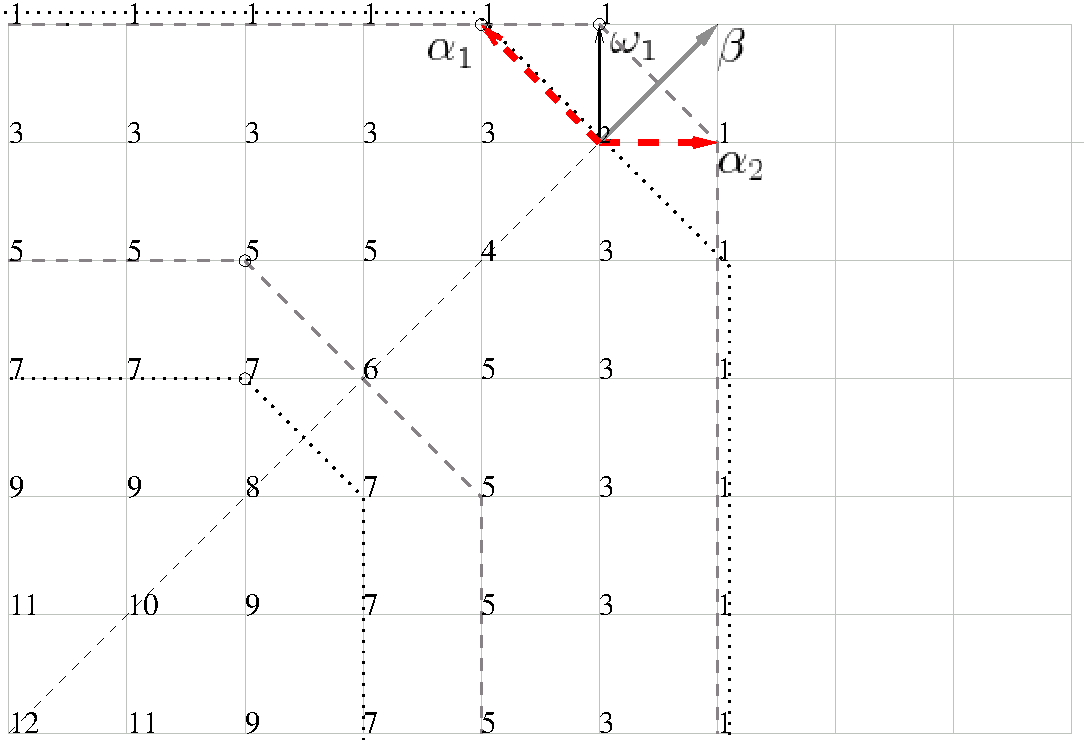
\includegraphics[width=120mm]{B2_Gen_Verma_Decomp}
  }
  \caption{Обобщенные модули Верма для регулярного вложения  $A_1$ в $B_2$. 
    Простые корни $\alpha_1, \alpha_2$ алгебры $B_2$ показаны пунктирными стрелками. Простой корень  $\beta = \alpha_1+2\alpha_2$ алгебры $A_1$ изображен серым вектором. Разложение $L^{\omega_{1}}$ представлено набором контуров входящих в него обобщенных модулей Верма. Пунктирные контуры соответствуют положительным значениям  $\epsilon(u)$, а точечные -- отрицательным. }

 \label{fig:B2_Verma_Decomp}
\end{figure}

\end{example}

\begin{remark}
Как доказано, например, в книге  \cite{humphreys2008representations} (см. утверждение 9.6), характеры обобщенных модулей Верма $M_{I}^{\mu _{\frak{a}_{\perp }}\left( u\right) }$ могут также описываться как линейные комбинации обычных модулей Верма алгебры $\frak{g}$:
\begin{equation*}
\mathrm{ch}M_{I}^{\mu _{\frak{a}_{\perp }}\left( u\right) }=\sum_{w\in W_{%
\frak{a}_{\perp }}}\epsilon \left( w\right) \mathrm{ch}M^{w\left( \mu _{%
\frak{a}_{\perp }}\left( u\right) +\rho _{\frak{a}_{\perp }}\right) -\rho _{%
\frak{a}_{\perp }}}
\end{equation*}
Подставляя это выражение в формулу (\ref{char in gen verma mod}) и используя определения  (\ref{mu-a},\ref{mu-a-tilda}) и (\ref{defect ort}), мы восстанавливаем стандартное разложение Вейля-Верма для характера:
\begin{equation*}
\mathrm{ch}\left( L^{\mu }\right) =\sum_{w\in W}\;\epsilon (u)\mathrm{ch}%
M^{w\left( \mu +\rho \right) -\rho }.
\end{equation*}
\end{remark}

\subsection{БГГ резольвента и ветвление}
В работе \cite{lepowsky1977generalization} показано, что для модуля старшего веса $L^{\mu }$, где $\mu \in P^{+}$, последовательность (обобщенная БГГ резольвента)
\begin{equation}
0\rightarrow M_{r}^{I}\overset{\delta _{r}}{\rightarrow }M_{r-1}^{I}\overset{%
\delta _{r-1}}{\rightarrow }\ldots \overset{\delta _{1}}{\rightarrow }%
M_{0}^{I}\overset{\varepsilon }{\rightarrow }L^{\mu }\rightarrow 0,
\label{resolution sequence}
\end{equation}
где
\begin{equation}
M_{k}^{I}=\bigoplus_{u\in U,\;\mathrm{length}\left( u\right)
=k}M_{I}^{u\left( \mu +\rho \right) -\rho },\quad M_{0}^{I}=M_{I}^{\mu }
\label{Verma elements sequence}
\end{equation}
является точной и формула (\ref{gen Weyl-Verma}%
) следует из этого разложения.

\begin{figure}[h!bt]
 \noindent\centering{
   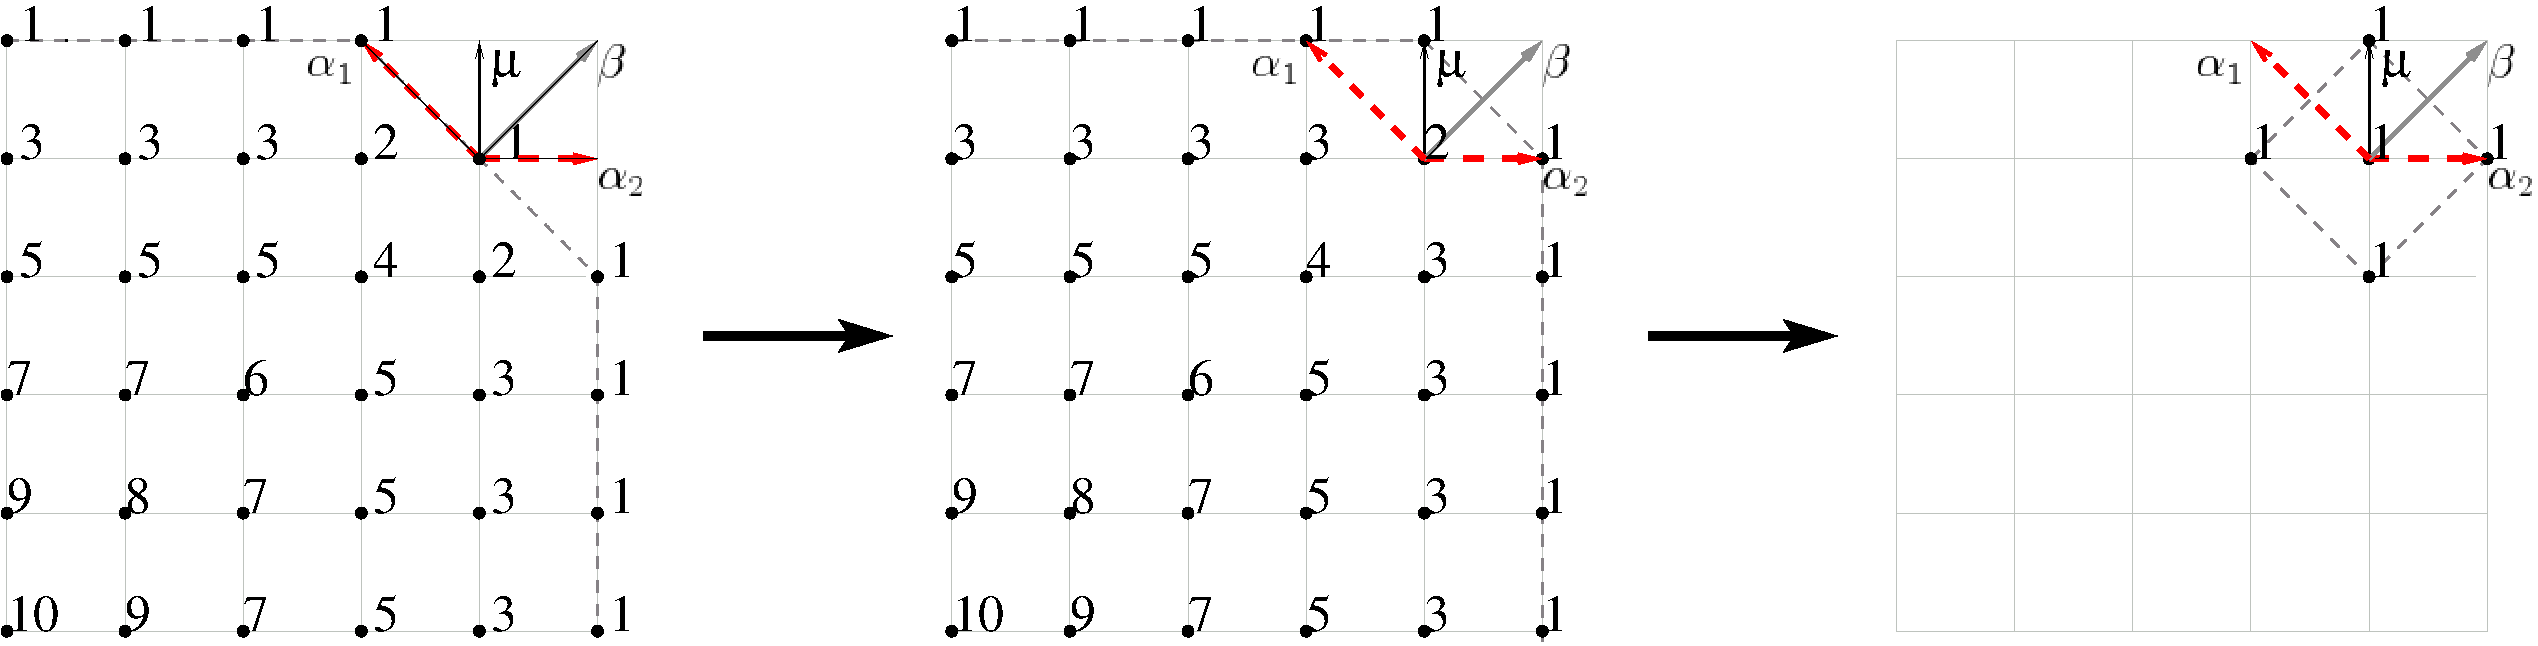
\includegraphics[width=140mm]{B2_Exact}}
 \caption{Вложение $A_1\hookrightarrow B_2$ (см. Рисунок \ref{fig:B2_Verma_Decomp}). Ортогональный партнер, подалгебра $A_1$, соответствует корню $\alpha_1$.
   Резольвента простого модуля $L^{\omega_1}$. Показана центральная часть точной последовательности
   $0 \to Im(\delta_2) \to \left( e^{\mu _{\widetilde{%
\frak{a}}}\left( e\right) }\mathrm{ch}M_{I}^{\pi _{\afb}\left[ \omega_1 \right] -%
\mathcal{D}_{\afb} }=M^{\omega_1}_{I}\right) \to
   L^{\omega_1}\to 0 $.  Здесь $\mu _{\widetilde{\frak{a}}}\left( e\right) =\pi _{\aft}\left[ \mu \right] + \mathcal{D}_{\afb}$.
   }
\end{figure}


\begin{statement}
Пусть $L^{\mu }$ --  $\frak{g}$-модуль со старшим весом $\mu \in P^{+}$, и пусть регулярная подалгебра  $\afb\hookrightarrow \frak{g}$ ортогональна редуктивной подалгебре $\frak{a}\hookrightarrow \frak{g}$. Тогда разложение (\ref{sing decomp main}) определяет как обобщенную резольвенту $L^{\mu }$ по отношению к $\afb$, так и правила ветвления $L^{\mu }$ по отношению к $\frak{a}_{\perp }$, так и правила ветвления $L^{\mu }$ по отношению к подалгебре $\frak{a}_{\perp }$, так и правила ветвления $L^{\mu }$ по отношению к $\frak{a}$ .
\end{statement}

\begin{proof}
Положим
\begin{equation*}
\mathrm{ch}M_{I}^{u\left( \mu +\rho \right) -\rho }=e^{\mu _{\widetilde{%
\frak{a}}}\left( u\right) }\mathrm{ch}M_{I}^{\mu _{\frak{a}_{\perp }}\left(
u\right) },\mathrm{ch}M_{I}^{\mu }=e^{\mu _{\widetilde{\frak{a}}}\left(
e\right) }\mathrm{ch}M_{I}^{\pi _{\frak{a}_{\perp }}\left[ \mu \right] -%
\mathcal{D}_{\frak{a}_{\perp }}},
\end{equation*}
где \ $\mu _{\widetilde{\frak{a}}}\left( u\right) ,\mu _{\frak{a}_{\perp
}}\left( u\right) $ и $\mathcal{D}_{\frak{a}_{\perp }}$ заданы как в Лемме \ref{Psi-decomp-lemma}, $%
u\in U$ определено формулой (\ref{U-def}). В результате получим элементы фильтрующей последовательности (\ref{resolution sequence}).

Рассмотрим множество $\left\{ \mu _{\frak{a}_{\perp }}\left( u\right) |u\in U\right\} $ как множество старших весов простых модулей $L_{\frak{a}%
_{\perp }}^{\mu _{\frak{a}_{\perp }}\left( u\right) }$ и вычислим размерности этих модулей. Вместе с 
$\left\{ \mu _{\widetilde{\mathfrak{a}}}\left( u\right) |u\in
U\right\} $ мы получим набор сингулярных весов
\begin{equation*}
\left\{ \epsilon (u)\;
e^{\mu _{\widetilde{\mathfrak{a}}}\left( u\right) }
\dim \left( L_{\frak{a}_{\perp }}^{\mu _{\frak{a}_{\perp
}}\left( u\right) }\right) \right\} .
\end{equation*}
Ветвление  $L_{\frak{g}\downarrow \frak{a}}^{\mu }=\bigoplus\limits_{\nu
\in P_{\frak{a}}^{+}}b_{\nu }^{\left( \mu \right) }L_{\frak{a}}^{\nu }$  определяется веером вложения  $\Gamma _{\frak{a}\rightarrow \frak{g}}$ и соотношением (\ref{recurrent rel}), которое дает нам коэффициенты  $k_{\xi
}^{\left( \mu \right) }$, а значит определяет и  $b_{\nu }^{\left( \mu \right) }$, так как  $b_{\nu }^{\left( \mu \right) }=k_{\nu }^{\left( \mu
\right) }$ при $\nu \in \overline{C_{\frak{a}}}$ .
\end{proof}

\begin{corollary}
Пусть  $L^{\mu }$ --  $\frak{g}$-модуль со старшим весом $\mu \in P^{+}$ и  $\frak{a}\hookrightarrow \frak{g}$ -- редуктивная подалгебра $\frak{g}$. Пусть $\frak{a}_{\perp }$, ортогональный партнер для $\frak{a}$, эквивалентен  $A_{1}$, $\frak{a}_{\perp }\approx $ $A_{1}$, и $\widetilde{\frak{a}}=\frak{a}\oplus \frak{h}_{\perp }$ с $\frak{h=\frak{h}_{\frak{a}}}\oplus \frak{h}_{\frak{a}_{\perp }}\oplus \frak{h}_{\perp }$. Пусть $L_{\frak{g}\downarrow \widetilde{\frak{a}}}^{\mu }=\bigoplus\limits_{\nu \in P_{\widetilde{\frak{a}}}^{+}}b_{\nu }^{\left( \mu \right) }L_{\widetilde{\frak{a}}}^{\nu }$ -- ветвление модуля $L^{\mu }$ относительно подалгебры $\widetilde{\frak{%
a}}$. Тогда коэффициенты $b_{\nu }^{\left( \mu \right) }$ определяют обобщенную резольвенту (\ref{resolution sequence}) модуля $L^{\mu }$
по отношению к  $\frak{a}_{\perp }$.
\end{corollary}

\begin{proof}
Пусть $\alpha $ -- простой корень  $A_{1}$. Используем преобразования из группы Вейля чтобы перевести его в некоторый простой корень алгебры $\frak{g}$, например $\alpha _{1}$. Построим сингулярный элемент для модуля  $L_{\frak{g}\downarrow
\widetilde{\frak{a}}}^{\mu }$, то есть  $\Psi _{\widetilde{\frak{a}}%
}^{\left( L_{\frak{g}\downarrow \widetilde{\frak{a}}}^{\mu }\right)
}=\sum_{\nu \in P_{\widetilde{\frak{a}}}^{+},b_{\nu }^{\left( \mu \right)
}>0}b_{\nu }^{\left( \mu \right) }\Psi _{\widetilde{\frak{a}}}^{\left( \nu
\right) }$, и разложим его $\Psi _{\widetilde{\frak{a}}}^{\left( L_{\frak{%
g}\downarrow \widetilde{\frak{a}}}^{\mu }\right) }=k_{\xi }^{\left( \mu
\right) }e^{\xi }$. В нашем случае представители $u$ в рекуррентном соотношении (\ref{recurrent rel}) определяются весом $\xi $ однозначно:
\begin{equation*}
\epsilon (u\left( \xi \right) )\;\dim \left( L_{\frak{a}_{\perp }}^{\mu _{%
\frak{a}_{\perp }}\left( u\left( \xi \right) \right) }\right) =-s\left(
\gamma _{0}\right) k_{\xi }^{\left( \mu \right) }-\sum_{\gamma \in \Gamma _{%
\widetilde{\frak{a}}\rightarrow \frak{g}}}s\left( \gamma +\gamma _{0}\right)
k_{\xi +\gamma }^{\left( \mu \right) }.
\end{equation*}
Тогда
\begin{equation*}
\dim \left( L_{\frak{a}_{\perp }}^{\mu _{\frak{a}_{\perp }}\left( u\left(
\xi \right) \right) }\right) =\left| s\left( \gamma _{0}\right) k_{\xi
}^{\left( \mu \right) }+\sum_{\gamma \in \Gamma _{\widetilde{\frak{a}}%
\rightarrow \frak{g}}}s\left( \gamma +\gamma _{0}\right) k_{\xi +\gamma
}^{\left( \mu \right) }\right|
\end{equation*}
и
\begin{equation*}
\mu _{\frak{a}_{\perp }}\left( u\left( \xi \right) \right) =\frac{1}{2}%
\left( \dim \left( L_{A_{1}}^{\mu \left( \xi \right) }\right) -1\right)
\alpha _{1}
\end{equation*}
Таким образом, множество обобщенных модулей Верма  $e^{\xi +\mathcal{D}%
_{\frak{a}_{\perp }}}\mathrm{ch}M_{I}^{\mu _{\frak{a}_{\perp }}\left(
u\left( \xi \right) \right) }$ полностью фиксировано:
\begin{equation*}
\left\{ e^{\mu _{\widetilde{\mathfrak{a}}}\left( u\right) }\mathrm{ch}%
M_{I}^{\mu _{\frak{a}_{\perp }}\left( u\right) }|u\in U\right\} .
\end{equation*}
Упорядочивая эти модули по длине $u$, мы получаем компоненты (\ref{Verma elements sequence}) резольвенты (\ref{resolution sequence}).
\end{proof}



\subsection{Заключение}

\label{sec:conclusions}
В работе \cite{2010arXiv1007.0318L} было показано, что метод веера вложения работает также и для специальных вложений. Надо заметить, что  разложения Вейля-Верма также могут быть получены в этом случае. Резольвенты, соответствующие специальным подалгебрам, описывают соотношения между проекциями характера начального модуля и обобщенными модулями Верма со старшими весами в подпространстве $h^*$.

Рассмотрим ситуацию, когда выбор простых корней зафиксирован какими-то внешними факторами (возникающими, например, из требований физических приложений). В этом случае ортогональный партнер не может порождаться только простыми корнями. Элементы   $\frak{u}_{I}^{+}:=\sum_{\eta \in \Delta
^{+}\setminus \Delta _{I}^{+}}\frak{g}_{\eta }$ не образуют подалгебру в  $%
\mathfrak{g}$, так как некоторые не простые корни отсутствуют в  $\Delta ^{+}\setminus
\Delta _{I}^{+}$. Важно отметить, что в этом случае формула Вейля-Верма по-прежнему существует. В ней обобщенные модули Верма соответствуют сжатиями \cite{Doebner1967Melsheimer} алгебры $%
\frak{n}^{+}$ и соотношения Вейля-Верма описывают разложение пространства представления $L^{\mu}$ в набор обобщенных модулей Верма сжатой алгебры  $U\left(\frak{n}_c^{+}\right)$. Весовые векторы образованы базисом Пуанкаре-Биркгофа-Витта алгебр $U\left(\frak{n}_c^{+}\right)$ и
$U\left( \mathfrak{a}_{\bot} \right)$. Чтобы рассмотреть такое пространство как  $%
\mathfrak{g}$-модуль мы должны выполнить деформацию \cite
{Nijenhuis1966Richardson} алгебры $\frak{n}_c^{+}$ (то есть восстановить первоначальный закон композиции). Пространство сохраняется, и после такой деформации генераторы начальной алгебры будут действовать на нем правильным образом.

\section{Сплинты и ветвления}
\label{sec:splints}


%%\newtheorem{Def}{Definition}[section]
%%\newtheorem{Cnj}[Def]{Conjecture}
%%\newtheorem{Prop}[Def]{Property}
%%\newtheorem{example}{Example}[section]
%%
%\input{tcilatex}


\begin{abstract}
Splint of root system for simple Lie algebra appears naturally in
studies of (regular) embeddings of reductive subalgebras. Splint can
be used to construct branching rules. We demonstrate that 
splint properties implementation drastically simplify calculations of
branching coefficients.
\end{abstract}

\section{Introduction}
\label{sec:Introduction}

Embedding $\phi$ of a root system $\Delta_1$ into a root system
$\Delta$ is a bijective map of roots of $\Delta_{1}$ to a (proper)
subset of $\Delta$ that commutes with vector composition law in
$\Delta_{1}$ and $\Delta$.
\begin{equation*}
\phi:\Delta_1 \longrightarrow \Delta
\end{equation*}
\begin{equation*}
\phi \circ (\alpha + \beta) =\phi \circ \alpha + \phi \circ \beta,
\,\,\, \alpha,\beta \in \Delta_1
\end{equation*}

Note that the image $Im(\phi)$ must not inherit the root system
properties except the addition rules equivalent to the addition
rules in $\Delta_{1}$ (for pre-images). Two embeddings $\phi_1$ and $\phi_2$  
can splinter $\Delta$  when the latter can be presented 
as a disjoint union of images $Im(\phi_1)$ and $Im(\phi_2)$.   
The term {\it splint} was
introduced by D. Richter in  \cite{richter2008splints} where the
classification of splints for simple Lie algebras was obtained.
There was also mentioned that splint must have tight
connections with the injection fan construction. The fan $\Gamma
\subset \Delta$ was
introduced in \cite{lyakhovsky1996rra} as a subset of root system describing recurrent
properties of branching coefficients for maximal embeddings. Injection fan is an
efficient tool to study branching rules. Later this construction
was generalized to non-maximal embeddings and infinite-dimensional
Lie algebras in \cite{2010arXiv1007.0318L, ilyin812pbc}.

In the present paper we study connections between splint and
injection fan for regular embedding of reductive subalgebras
${\mathfrak a}$ in simple Lie algebra $\mathfrak{g}$. We show that (under
certain conditions described in section \ref{sec:stems and
multiplicity functions}) splint is a natural tool to study
reduction properties of ${\mathfrak g}$-modules
with respect to a subalgebra ${\mathfrak a}\longrightarrow
{\mathfrak g}$. Using this tool we obtain the main result -- the one-to-one correspondence between weight
multiplicities in irreducible modules of splint and branching
coefficients for a reduced module $L^{\mu}_{{\mathfrak
g}\downarrow {\mathfrak a}}$.


\section{Injections and splints}

\label{sec:Injections and splints}

Consider a simple Lie algebra $\mathfrak{g}$ and its regular subalgebra $%
\mathfrak{a}\hookrightarrow \mathfrak{g}$ such that $\mathfrak{a}$
is a
reductive subalgebra $\mathfrak{a \subset g}$ with correlated root spaces: $%
\mathfrak{h}_{\mathfrak{a}}^{\ast }\subset \mathfrak{h}_{\mathfrak{g }%
}^{\ast }$. Let $\mathfrak{a}^{\mathfrak{s}}$ be a semisimple summand of
$\mathfrak{a}$,
this means that $\mathfrak{a}=\mathfrak{a}^{\mathfrak{s}} \oplus \mathfrak{u}(1)\oplus %
\mathfrak{u}(1)\oplus \dots$. We shall consider $\mathfrak{a}^{\mathfrak{s}}$
to be a proper regular subalgebra and $\mathfrak{a}$ to be the
maximal subalgebra with $\mathfrak{a}^{\mathfrak{s}}$ fixed that is the rank
$r$ of $\frak{a}$ is equal to that of $\mathfrak{g}$.

The following notations are used:

$r$ , $\left( r_{\mathfrak{a}^{\mathfrak{s}}}\right) $ --- the rank of
$\frak{g}$ $\left( \mathrm{{resp. }\mathfrak{a}^{\mathfrak{s}}}\right) $ ;

$\Delta $ $\left( \Delta _{\frak{a}}\right) $--- the root system;
$\Delta ^{+} $ $\left( \mathrm{{resp. }\Delta
_{\frak{a}}^{+}}\right) $--- the positive root system (of
$\frak{g}$ and $\frak{a}$ respectively);

$S \, ,\quad \left( S_{\frak{a}}\right) $ --- the system of simple roots (of $%
\frak{g}$ and $\frak{a}$ respectively);

$\alpha _{i}$ , $\left( \alpha _{\left( \frak{a}\right) j}\right) $ --- the $%
i$-th (resp. $j$-th) simple root for $\frak{g}$  $\left( \mathrm{{resp. \,} \frak{%
a}}\right) $; $i=0,\ldots ,r$,\ \ $\left( j=0,\ldots ,r_{\mathfrak{a}%
^S}\right) $;

$\omega _{i}$ , $\left( \omega _{\left( \frak{a}\right) j}\right) $ --- the $%
i$-th (resp. $j$-th) fundamental weight for $\frak{g}$ $\left( \mathrm{{resp. \,}\frak{%
a}}\right) $; $i=0,\ldots ,r$,\ \ $\left( j=0,\ldots ,r_{\mathfrak{a}%
^S}\right) $;

$W$ , $\left( W_{\frak{a}}\right) $--- the corresponding Weyl group;

$C$ , $\left( C_{\frak{a}}\right) $--- the fundamental Weyl chamber;

$\bar{C}, \left(\bar{C_{\frak{a}}}\right)$ --- the closure of the
fundamental Weyl chamber;

$\epsilon \left( w\right) :=\left( -1\right) ^{\mathrm{length}(w)}$;

$\rho $\ , $\left( \rho _{\frak{a}}\right) $\ --- the Weyl vector;

$L^{\mu }$\ $\left( L_{\frak{a}}^{\nu }\right) $\ --- the integrable module
of $\frak{g}$ with the highest weight $\mu $\ ; (resp. integrable $\frak{a}$
-module with the highest weight $\nu $ );

$\mathcal{N}^{\mu }$ , $\left( \mathcal{N}_{\frak{a}}^{\nu }\right) $ ---
the weight diagram of $L^{\mu }$ (resp. ${}L_{\frak{a}}^{\nu }$ );

$P$ (resp. $P_{\frak{a}} $) \ --- the weight lattice;

$P^{+}$ (resp. $P_{\frak{a}}^{+} $) \ --- the dominant weight lattice;

$\mathcal{E}$ (resp. $\mathcal{E}_{\frak{a}} $) \ --- the formal algebra;

$m_{\xi }^{\left( \mu \right) }$ , $\left( m_{\xi }^{\left( \nu \right)
}\right) $ --- the multiplicity of the weight $\xi \in P$ \ $\left( \mathrm{{%
resp. }\in P_{\frak{a}}}\right) $ in the module $L^{\mu }$ , (resp. $\xi \in
L_{\frak{a}}^{\nu } $);

$ch\left( L^{\mu }\right) $ (resp. $\mathrm{ch}\left( L_{\frak{a}}^{\nu
}\right) $)--- the formal character of $L^{\mu }$ (resp. $L_{\frak{a}}^{\nu
} $);

$ch\left( L^{\mu }\right)  =\frac{\sum_{w\in W}\epsilon (w)e^{w\circ (\mu
+\rho )-\rho }} {\prod_{\alpha \in \Delta ^{+}} \left( 1-e^{-\alpha }\right)
} $ --- the Weyl formula;

$R:=\prod_{\alpha \in \Delta ^{+}}\left( 1-e^{-\alpha }\right) \quad $
(resp. $R_{\frak{a}}: =\prod_{\alpha \in \Delta_{\frak{a}}^{+}} \left(
1-e^{-\alpha }\right) $ ) --- the Weyl denominator.

Let $L^{\mu }$ be completely reducible with respect to $\frak{a}$,
\[
L_{\frak{g}\downarrow \frak{a}}^{\mu }=\bigoplus\limits_{\nu \in P_{\frak{a}%
}^{+}}b_{\nu }^{\left( \mu \right) }L_{\frak{a}}^{\nu }.
\]
\begin{equation}
\pi _{\frak{a}}ch\left( L^{\mu }\right) =\sum_{\nu \in P_{\frak{a}%
}^{+}}b_{\nu }^{(\mu )}ch\left( L_{\frak{a}}^{\nu }\right) .
\label{branching1}
\end{equation}
For the modules we are interested in the Weyl formula for $\mathrm{ch}\left(
L^{\mu }\right) $ can be written in terms of singular elements \cite
{humphreys1997introduction}
\[
\Psi ^{\left( \mu \right) }:=\sum\limits_{w\in W}\epsilon (w)e^{w(\mu +\rho
)-\rho },
\]
namely,
\begin{equation}
\mathrm{ch}\left( L^{\mu }\right) =\frac{\Psi ^{\left( \mu \right) }}{\Psi
^{\left( 0\right) }}=\frac{\Psi ^{\left( \mu \right) }}{R}.
\label{Weyl-Kac2}
\end{equation}
The same is true for submodules $\mathrm{ch}\left( L_{\frak{a}}^{\nu
}\right) $ in (\ref{branching1})
\[
\mathrm{ch}\left( L_{\frak{a}}^{\nu }\right) =\frac{\Psi _{\frak{a}}^{\left(
\nu \right) }}{\Psi _{\frak{a}}^{\left( 0\right) }}=\frac{\Psi _{\frak{a}%
}^{\left( \nu \right) }}{R_{\frak{a}}},
\]
with
\[
\Psi _{\frak{a}}^{\left( \nu \right) }:=\sum\limits_{w\in W_{\frak{a}%
}}\epsilon (w)e^{w(\nu +\rho _{_{\frak{a}}})-\rho _{_{\frak{a}}}}.
\]

Applying formula (\ref{Weyl-Kac2}) to the branching rule (\ref{branching1})
we get a relation connecting the singular elements $\Psi ^{\left( \mu
\right) }$ and $\Psi _{\frak{a}}^{\left( \nu \right) }$ :
\begin{eqnarray}
\frac{\sum_{w \in W}\epsilon (w )e^{w (\mu +\rho )-\rho }}{\prod_{\alpha \in
\Delta ^{+}}(1-e^{-\alpha })} &=&\sum_{\nu \in P_{\frak{a}}^{+}}b_{\nu
}^{(\mu )}\frac{\sum_{w \in W_{\frak{a}}}\epsilon (w )e^{w (\nu +\rho _{%
\frak{a}})-\rho _{\frak{a}}}}{\prod_{\beta \in \Delta _{\frak{a}%
}^{+}}(1-e^{-\beta })},  \nonumber  \label{eq:4} \\
\frac{\Psi ^{\left( \mu \right) }}{R} &=&\sum_{\nu \in P_{\frak{a}%
}^{+}}b_{\nu }^{(\mu )}\frac{\Psi _{\frak{a}}^{\left( \nu \right) }}{R_{%
\frak{a}}}.  \label{singular main}
\end{eqnarray}

In \cite{2010arXiv1007.0318L} it was proven that branching coefficients $%
b_{\xi }^{\left( \mu \right) }$ corresponding to the injection $\frak{a}%
\hookrightarrow \frak{g}$ are subject to the set of recurrent relations:
\begin{equation}
\begin{array}{c}
b_{\xi }^{\left( \mu \right) }=-\frac{1}{s\left( \gamma _{0}\right) }\left(
\sum_{u\in W/W_{\perp}}\epsilon (u)\;\dim \left( L_{\frak{a}_{\perp }}^{\mu _{\frak{a}%
_{\perp }}\left( u\right) }\right) \delta _{\xi -\gamma _{0},\pi _{%
\widetilde{\frak{a}}}(u(\mu +\rho )-\rho )}+\right. \\
\left. +\sum_{\gamma \in \Gamma _{\widetilde{\frak{a}}\rightarrow \frak{g}%
}}s\left( \gamma +\gamma _{0}\right) b_{\xi +\gamma }^{\left( \mu \right)
}\right) .
\end{array}
\label{recurrent rel}
\end{equation}
where $\frak{a}_{\perp }$ is the subalgebra determined by the roots of $%
\frak{g}$ orthogonal to roots of $\frak{a}$ and $W_{\perp}$ is a Weyl group of $\mathfrak{a}_{\perp}$
\begin{eqnarray}
\Delta _{\frak{a}_{\perp }} &:&=\left\{ \beta \in \Delta _{\frak{g}}|\forall
h\in \frak{h}_{\frak{a}};\beta \left( h\right) =0\right\} ,
\label{delta a ort}
\end{eqnarray}
\begin{eqnarray}
\widetilde{\frak{a}_{\perp }} :=\frak{a}_{\perp }\oplus \frak{h}_{\perp }
\qquad \widetilde{\frak{a}} :=\frak{a}\oplus \frak{h}_{\perp }
\end{eqnarray}
and $\pi$ is the projection operator. When an injection is maximal the
projection becomes trivial and the relation (\ref{recurrent rel}) is
simplified:
\begin{equation}
\begin{array}{c}
b_{\xi }^{\left( \mu \right) }=-\frac{1}{s\left( \gamma _{0}\right) }\left(
\sum_{u\in W}\epsilon (u) \delta _{\xi -\gamma _{0}, u(\mu +\rho )-\rho
}+\right. \\
\left. +\sum_{\gamma \in \Gamma _{\frak{a}\rightarrow \frak{g}}}s\left(
\gamma +\gamma _{0}\right) b_{\xi +\gamma }^{\left( \mu \right) }\right) .
\end{array}
\label{recurrent relation max}
\end{equation}
The recursion is goverened by the set $\Gamma _{\frak{a}\rightarrow \frak{g}}
$ called the injection fan. The latter is defined by the carrier set $%
\left\{ \xi \right\} _{\frak{a}\rightarrow \frak{g}}$ for the coefficient
function $s(\xi )$
\[
\left\{ \xi \right\} _{\frak{a}\rightarrow \frak{g}}:=\left\{ \xi \in P_{%
\frak{a}}|s(\xi )\neq 0\right\}
\]
appearing in the expansion
\begin{equation}
\prod_{\alpha \in \Delta ^{+}\setminus \Delta _{\frak{a}}^{+}}\left( 1-e^{
-\alpha }\right) =-\sum_{\gamma \in P_{\frak{a}}}s(\gamma )e^{-\gamma };\quad
\label{product}
\end{equation}

Now we remind two definitions introduced in \cite{richter2008splints}

\begin{Def}
Suppose $\Delta _{0}$ and $\Delta $ are root systems with corresponding
weight lattices $P_{0}$ and $P$. Then $\phi $ is an ``embedding'',
\begin{equation}
\phi :\left\{
\begin{array}{l}
\Delta _{0}\hookrightarrow \Delta , \\
P_{0}\hookrightarrow P,
\end{array}
\right.
\end{equation}
if \newline
\noindent (a) it injects $\Delta _{0}$ in $\Delta $, and \newline
\noindent (b) acts homomorphically with respect to the vector groups in $%
P_{0}$ and $P$:
\[
\phi (\gamma )=\phi (\alpha )+\phi (\beta )
\]
for any triple $\alpha ,\beta ,\gamma \in P_{0}$ such that $\gamma =\alpha
+\beta $.
\end{Def}

$\phi$ induces an injection of formal algebras $:{\mathcal{E}}_0
\hookrightarrow \mathcal{E}$ and for the image ${\mathcal{E}}%
_i=Im_{\phi}\left( {\mathcal{E}}_0\right)$ one can consider its inverse $%
\phi^{-1}:{\mathcal{E}}_i \longrightarrow {\mathcal{E}}_0$.

Notice that one must distinguish two classes of embeddings: when the scalar
product (defined by the Killing form) in the root space $P_0$ is invariant
with respect to $\phi$ and when it is not $\phi$-invariant. The first
embedding is called "metric" , the second -- "nonmetric".

\begin{Def}
A root system $\Delta $ ''splinters'' as $(\Delta _{1},\Delta _{2})$ if
there are two embeddings $\phi _{1}:\Delta _{1}\hookrightarrow \Delta $ and $%
\phi _{2}:\Delta _{2}\hookrightarrow \Delta $ where (a) $\Delta $ is the
disjoint union of the images of $\phi _{1}$ and $\phi _{2}$ and (b) neither
the rank of $\Delta _{1}$ nor the rank of $\Delta _{2}$ exceeds the rank of $%
\Delta $.
\end{Def}

It is equivalent to say that $(\Delta_1,\Delta_2)$ is a "splint'' of $\Delta$
and we shall denote this by $\Delta \approx (\Delta_1,\Delta_2)$. Each
component $\Delta_1$ and $\Delta_2$ is a "stem'' of the splint $%
(\Delta_1,\Delta_2)$.

To study relations between injection fan technique and splint let us 
consider the case when one of the stems $\Delta _{1}=\Delta _{\frak{a}}$ 
is a root subsystem.

Splint $\Delta \approx (\Delta _{1},\Delta _{2})$ is called ''injective'' if
$\Delta _{1}=\Delta _{\frak{a}}$, is a root subsystem
in $\Delta $ corresponding to a regular reductive subalgebra $\frak{a}%
\hookrightarrow \frak{g}$.

In case of injective splint the second stem $\Delta _{\frak{s}}:=\Delta
_{2}=\Delta \setminus \Delta _{\frak{a}}$ can be translated into a product (%
\ref{product}) and it defines an injection fan $\Gamma _{\frak{a}%
\hookrightarrow \frak{g}}$. Denote by $\Delta_{\mathfrak{s}0}$ the coimage of the second embedding $\phi:\Delta_{\mathfrak{s}0}\to \Delta_{\mathfrak{g}}$.
The following conjecture follows.

\begin{Cnj}
Each injective splint $\Delta \approx (\Delta _{\frak{a}},\Delta _{\frak{s}})
$ defines an injection fan with the carrier $\left\{ \xi \right\} _{\frak{a}%
\rightarrow \frak{g}}$ fixed by the product
\begin{equation}
\prod_{\beta \in \Delta _{\frak{s}}^{+}}\left( 1-e^{-\beta }\right)
=-\sum_{\gamma \in P}s(\gamma )e^{-\gamma }\quad   \label{splint product}
\end{equation}
\end{Cnj}

In case of injective splint we say that subalgebra $\frak{a}\hookrightarrow \frak{g}$
splinters $\Delta $ (and call $\frak{a}$ the ''splinting subalgebra'' of $%
\frak{g}$). In \cite{richter2008splints} splints are classified (see Appendix there)
and the first three types of them are injective.

\section{How stems define multiplicity functions}

\label{sec:stems and multiplicity functions}

In this Section we study properties of injective splints  $\Delta \approx (\Delta _{\frak{a}},\Delta _{\frak{s}})
$. It will
be demonstrated that in this case to find branching
coefficients for a splinting injection $\frak{a}\hookrightarrow
\frak{g}$ means to find weight multiplicities of an irreducible
$\frak{s}$-module $L_{\frak{s}}^{\nu }$ with fixed highest weight
$\nu $. Notice that $\frak{s}$ must not be a subalgebra of
$\frak{g}$.

Let us return to relation (\ref{singular main}) and multiply both sides by $%
R_{\frak{a}}$:
\begin{equation}
\frac{1}{\prod_{\beta \in \Delta _{\frak{s}}^{+}}(1-e^{-\beta })}\Psi _{%
\frak{g}}^{\left( \mu \right) }=\sum_{\nu \in P_{\frak{a}}^{+}}b_{\nu
}^{(\mu )}\Psi _{\frak{a}}^{\left( \nu \right) }.
\label{singular main-2}
\end{equation}
Here the first factor in the l.h.s. is the inverse of the fan $\Gamma _{%
\frak{a}\rightarrow \frak{g}}$. Consider the highest weight module $L_{\frak{%
s}}^{\nu }$. The embedding $\phi :\Delta _{\frak{s}\,0}\longrightarrow \Delta
_{\frak{g}}$ sends the singular element $\Psi _{\frak{s}}^{\left( \nu
\right) }$ into $\Psi _{\frak{g}}^{\left( \mu \right) }$. Applying the
inverse morphism $\phi ^{-1}$ to the product $\left( \prod_{\beta \in \Delta
_{\frak{s}}^{+}}(1-e^{-\beta })\right) ^{-1}\phi \left( \Psi _{\frak{s}%
}^{\left( \nu \right) }\right) $ one gets the character of the module $L_{%
\frak{s}}^{\nu }$,

\begin{equation}
\phi ^{-1}\left( \frac{1}{\prod_{\beta \in \Delta _{\frak{s}%
}^{+}}(1-e^{-\beta })}\phi \left( \Psi _{\frak{s}}^{\left( \nu \right)
}\right) \right) =\frac{1}{\prod_{\beta \in \Delta _{\frak{s}0
}^{+}}(1-e^{-\beta })}\Psi _{\frak{s}}^{\left( \nu \right) }=\mathrm{ch}%
\left( L_{\frak{s}}^{\nu }\right) .  \label{inverse for stem}
\end{equation}
Our task is to prove that the singular element $\Psi _{\frak{g}}^{\left( \mu
\right) }$ contains the element $\Psi _{\frak{s}}^{\left( \xi \right) }$ for
a module $L_{\frak{s}}^{\xi }$ uniquely defined by $L_{\frak{g}}^{\mu }$ and
that the branching coefficients $b_{\nu }^{(\mu )}$ in the r.h.s. of (\ref
{singular main-2}) coincide with multiplicities $m_{\zeta }^{\left( \xi
\right) }$ of the corresponding weights in $\mathcal{N}_{\frak{s}}^{\xi }$ .

For a highest weight irreducible module $L_{\frak{g}}^{\mu }$ the singular
element $\Psi _{\frak{g}}^{\left( \mu \right) }$ is an element of $\mathcal{E%
}$ corresponding to the shifted Weyl-orbit of the weight $\left( \mu +\rho
\right) \in P^{+}$ with the sign function $\epsilon \left( w\right) $. It is
convenient to use also unshifted singular elements
\begin{equation}
\Phi ^{\left( \mu \right) }:=\Psi ^{\left( \mu \right) }e^{\rho }.
\label{definition Phi}
\end{equation}
In these terms the relation (\ref{singular main-2}) looks like
\begin{equation}
\frac{e^{\rho _{\frak{g}}-\rho _{\frak{a}}}}{\prod_{\beta \in \Delta _{\frak{%
s}}^{+}}(1-e^{-\beta })}\Phi _{\frak{g}}^{\left( \mu \right) }=\sum_{\nu \in
P_{\frak{a}}^{+}}b_{\nu }^{(\mu )}\Phi _{\frak{a}}^{\left( \nu \right) }.
\label{singular main-3}
\end{equation}
The orbit related to $\Phi _{\frak{g}}^{\left( \mu \right) }$ is completely
defined by the set of edges $\left\{ \lambda _{i}\right\} _{i=1,\dots ,r}$
adjusted to the end of the highest weight vector $\mu +\rho $. For $\mu
=\sum m_{i}\omega _{i}$ these edges are
\begin{equation}
\lambda _{i}=-\left( m_{i}+1\right) \alpha _{i},\quad i=1,\dots ,r.
\label{edge}
\end{equation}
Each formal exponent $e^{\mu +\rho +\lambda _{i}}$ in $\Phi _{\frak{g}%
}^{\left( \mu \right) }$ bears the sign coefficient $\epsilon =(-)$. The
defining property of $\Phi _{\frak{g}}^{\left( \mu \right) }$ is as follows.
Consider any pair of edges $\lambda _{i},\lambda _{j}$ and the corresponding
weights $\mu +\rho $, $\mu +\rho +\lambda _{i}$ and $\mu +\rho +\lambda _{j}$. 
Apply the reflection $s_{\alpha _{i}}$ (or $s_{\alpha _{j}}$),
\begin{equation}
s_{\alpha _{i}}\circ \left\{
\begin{array}{l}
\left( \mu +\rho \right)  \\
\left( \mu +\rho +\lambda _{i}\right)  \\
\left( \mu +\rho +\lambda _{j}\right)
\end{array}
\right. =\left\{
\begin{array}{l}
\left( \mu +\rho +\lambda _{i}\right)  \\
\left( \mu +\rho \right)  \\
\left( \mu +\rho +\lambda _{i}-(m_{j}+1)s_{\alpha _{i}}\circ \alpha
_{j}\right)
\end{array}
\right.   \label{reflected triple}
\end{equation}

\begin{Prop}
The edge $\lambda _{i,j}$ of $\Phi _{\frak{g}}^{\left( \mu \right) }$
starting at the weight $\left( \mu +\rho +\lambda _{i}\right) $ along the
root $-s_{\alpha _{i}}\circ \alpha _{j}$ has the same length in $(s_{\alpha
_{i}}\circ \alpha _{j})$ as $\lambda _{j}$ has in $\alpha _{j}$. (The same
is true for the edge $\lambda _{j,i}$, its length in $(s_{\alpha _{j}}\circ
\alpha _{i})$ is equal to the length of $\lambda _{i}$ in $\alpha _{i}$.)
\label{diagram property}
\end{Prop}

In $\Phi _{\frak{g}}^{\left( \mu \right) }$ the elements $e^{\left( \mu
+\rho +\lambda _{i}-(m_{j}+1)s_{\alpha _{i}}\circ \alpha _{j}\right) }$ and $%
e^{\left( \mu +\rho +\lambda _{j}-(m_{i}+1)s_{\alpha _{j}}\circ \alpha
_{i}\right) }$ have the sign coefficient  $\epsilon =(+)$.

Remember that only three types of splints are
injective and thus are naturally connected with branching. Below we
reproduce the part of the splints table from \cite{richter2008splints} corresponding to
injective splints:
\[
\begin{array}{cc||c|c}
\hbox{type} & \hspace{0.25in}\Delta \hspace{0.25in} & \hspace{0.25in}\Delta
_{\frak{a}}\hspace{0.25in} & \hspace{0.25in}\Delta _{\frak{s}}\hspace{0.25in}
\\ \hline\hline
\hbox{(i)} & G_{2} & A_{2} & A_{2} \\
& F_{4} & D_{4} & D_{4} \\ \hline
\hbox{(ii)} & B_{r}(r\geq 2) & D_{r} & \oplus ^{r}A_{1} \\
& C_{r}(r\geq 3) & D_{r} & \oplus ^{r}A_{1} \\ \hline
\hbox{(iii)} & A_{r}(r\geq 2) & A_{r-1}\oplus u\left( 1\right)  & \oplus
^{r}A_{1} \\
& B_{2} & A_{1}\oplus u\left( 1\right)  & A_{2}
\end{array}
\]
Each row in the table gives a splint $(\Delta _{\frak{a}},\Delta _{\frak{s}})
$ of the simple root system $\Delta $. In the first two types both $\Delta _{%
\frak{a}}$ and $\Delta _{\frak{s}}$ are embedded metrically. Stems in the
first type splints are equivalent and in the second are not. In the third
type splints only $\Delta _{\frak{a}}$ is embedded metrically. The summands $%
u\left( 1\right) $ are added to keep $r_{\frak{a}}=r$. This does not change
the principle properties of branching but makes it possible to use the
multiplicities of $\frak{s}$-modules without further projecting their
weights.

Splints induce a decomposition of the set $S=S_{\frak{c}}\cup S_{\frak{d}}$
with $S_{\frak{c}}=S\cap S_{\frak{a}}$ and $S_{\frak{d}}=S\cap S_{\frak{s}}$. 
It is easy to check that for any injective splint the subset $S_{%
\frak{d}}$ is nonempty. It follows that in the set $\left\{ \lambda
_{i}\right\} _{i=1,\dots ,r}$ one can always find simple roots $\beta
_{k}\in \Delta _{\frak{s}}$ and that the orbit corresponding to $\Phi _{%
\frak{g}}^{\left( \mu \right) }$ contains the edges
\begin{equation}
\lambda _{k}=-\left( m_{k}+1\right) \beta _{k}  \label{beta edge}
\end{equation}
attached to the weight $\mu +\rho $. As far as $\Delta _{\frak{a}}$ is a
root system and for any pair of simple roots from $S_{\frak{c}}$ the
property \ref{diagram property} is fulfilled, the element $\Phi _{\frak{g}%
}^{\left( \mu \right) }$ being a singular element for a set of $\frak{a}$%
-modules. Consider $\beta _{l}\in \Delta _{\frak{s}}$ whose coimage in $%
\Delta _{\frak{s}0}$ is simple. In Appendix it is shown that for any such $%
\beta _{l}$ there exists a root $\alpha _{l}\in S_{\frak{c}}$ such that
$\beta _{l}=\alpha _{l}+\beta _{k}$. It is easily seen that the
corresponding edge intersects the boundary plane of the fundamental chamber $%
\bar{C_{\frak{a}}}$ orthogonal to the root $\alpha _{l}$,
\begin{equation}
s_{\alpha _{l}}\left( \mu +\rho -p\beta _{l}\right) =s_{\alpha _{l}}\left(
\mu +\rho \right) -ps_{\alpha _{l}}\beta _{l}=\mu +\rho -p\beta _{l},
\label{intersection}
\end{equation}
\begin{equation}
\mu +\rho -s_{\alpha _{l}}\left( \mu +\rho \right) =\left( m_{l}+1\right)
\alpha _{l}=\left( m_{l}+1\right) \beta _{l}-\left( m_{l}+1\right) \beta
_{k}=p\beta _{l}-ps_{\alpha _{l}}\beta _{l}.  
\label{intersection-2}
\end{equation}
It follows that $p=\left( m_{l}+1\right) $ and $s_{\alpha _{l}}\beta
_{l}=\beta _{k}$. Now apply the operator $s_{\beta _{k}}$ and find that the
edge along the root $s_{\beta _{k}}\alpha _{l}$ attached at the weight $%
s_{\beta _{k}}(\mu +\rho )$ is also equal to $-ps_{\beta _{k}}\alpha _{l}$.
This means that for the triple of roots $\beta _{k},\beta _{l}$ and $%
s_{\beta _{k}}\alpha _{l}$ in $\Delta _{\frak{s}}$ the edges $\lambda
_{k}=-\left( m_{k}+1\right) \beta _{k}$, $\lambda _{l}=-\left(
m_{l}+1\right) \beta _{l}$ and $\lambda _{kl}=-\left( m_{l}+1\right)
s_{\beta _{k}}\alpha _{l}$ demonstrate the property \ref{diagram property}.
One can continue this procedure further in the 2-dimensional subspace fixed
by the roots $\beta _{k}$ and $\beta _{l}$ and find the set of formal
exponents that being supplied with the corresponding sign factors compose
the coimage of the singular element of a module for the subalgebra in $\frak{%
s}$ (this subalgebra has rank $r=2$).

The same can be proven for any positive root $\beta _{l}\in \Delta $ that is
simple in $\Delta _{\frak{s}0}$ and correspondingly for any $r=2$ subalgebra
in $\frak{s}$. The latter means that to ''find'' a singular element of $%
\frak{s}$-module in $\Phi _{\frak{g}}^{\left( \mu \right) }$ it is necessary
to incorporate in it additional formal elements $\left\{ -e^{\mu +\rho
-\left( m_{l}+1\right) \beta _{l}}|\beta _{l}\in S_{\frak{c}}\right\}.$ This
fixes the starting edges of the diagram $\phi ^{-1}\left( \Phi _{\frak{s}}^{%
\widetilde{\mu }}\right) $. As it follows from the reconstruction procedure
the highest weight $\widetilde{\mu }$ is totally defined by the weight $\mu $%
, they have the same Dynkin numbers:
\begin{equation}
\mu =\sum m_{k}\omega _{k}\qquad \Longrightarrow \quad \widetilde{\mu }=\sum
m_{k}\widetilde{\omega }_{k} . \label{new h weight}
\end{equation}
The next step is to construct the full $W_{\frak{s}}$-orbit $\Phi _{\frak{s}%
}^{\left( \widetilde{\mu }\right) }$  in $P_{\frak{s}}$. It is easily seen
that its coimage belongs to $\bar{C_{\frak{a}}}$ and that the set $\phi
^{-1}\left( \Phi _{\frak{s}}^{\widetilde{\mu }}\right) \setminus \Phi _{%
\frak{g}}^{\left( \mu \right) }|_{\bar{C_{\frak{a}}}}$ corresponds to the
weights belonging to the boundary $\bar{C_{\frak{a}}}$ (including the subset
$\left\{ -e^{\mu +\rho -\left( m_{l}+1\right) \beta _{l}}|\beta _{l}\in S_{%
\frak{c}}\right\} $). Thus we have constructed all the formal elements\ with
the appropriate sign factors that after being added to $\Phi _{\frak{g}%
}^{\left( \mu \right) }|_{\bar{C_{\frak{a}}}}$ form the diagram $\phi
^{-1}\left( \Phi _{\frak{s}}^{\widetilde{\mu }}\right) $ in $\bar{C_{\frak{a}%
}}$.

Now let us return to relation (\ref{singular main-3}). One can add to $%
\Phi _{\frak{g}}^{\left( \mu \right) }$ pairs of formal elements
constructed above  with the opposite signs: $\epsilon \left( w\right)
|_{w\in W_{\frak{s}}}$ and $-\epsilon \left( w\right) |_{w\in W_{\frak{s}}}$. 
Attribute the signs $\epsilon \left( w\right) |_{w\in W_{\frak{s}}}$ to
the elements whose weights we shall attribute to $\bar{C_{\frak{a}}}$. 
The same elements with the opposite signs are to be referred to the
neighboring Weyl chambers of $\bar{C_{\frak{a}}^{(l)}}$ (the latter are
connected with the main one via simple reflections $s_{\alpha _{l}}$ so the
signes $-\epsilon \left( w\right) |_{w\in W_{\frak{s}}}$ are natural for
them). In fact one can repeat the procedure and find additional singular
weights in any Weyl chamber $\bar{C_{\frak{a}}^{(m)}}$ and in them
additional singular weights always have the signs opposite to that in their
nearest neighbors. Thus without changing the element $\Phi _{\frak{g}%
}^{\left( \mu \right) }$ one can present it as a sum
\begin{equation}
\Phi _{\frak{g}}^{\left( \mu \right) }=\sum_{w\in W_{\frak{a}}}w\circ \left(
e^{\rho _{\frak{a}}}\Psi ^{\widetilde{\mu }+\rho _{\frak{s}}}\right)
\label{singular final}
\end{equation}
where the weight $\widetilde{\mu }=\sum m_{k}\omega _{\frak{s}}^{k}$ was
defined above. The decomposition (\ref{singular final}) provides the
possibility to apply the factor $\left( \prod_{\beta \in \Delta _{\frak{s}%
}^{+}}(1-e^{-\beta })\right) ^{-1}$ to each summand of the singular element $%
\Phi _{\frak{g}}^{\left( \mu \right) }$ separately because the sets of
weights from different Weyl summands do not intersect. Taking into account
the isomorphism $\phi $ one can see that in the main Weyl chamber $\bar{C_{%
\frak{a}}}$ the set of weights generated by the factor $\left( \prod_{\beta
\in \Delta _{\frak{s}}^{+}}(1-e^{-\beta })\right) ^{-1}$ is isomorphic to
the weight diagram $\mathcal{N}_{\frak{s}}^{\widetilde{\mu }}$ of the $\frak{%
s}$-module $L_{\frak{s}}^{\widetilde{\mu }}$. Now one can restrict
relation (\ref{singular main-3}) to $\bar{C_{\frak{a}}}$ and obtain the main
result:
\begin{Prop}
\begin{equation}
\frac{e^{\rho _{\frak{g}}}}{\prod_{\beta \in \Delta _{\frak{s}%
}^{+}}(1-e^{-\beta })}\left( \Psi ^{\widetilde{\mu }+\rho _{\frak{s}%
}}\right) =\sum_{\widetilde{\nu }\in \mathcal{N}_{\frak{s}}^{\widetilde{\mu }%
}}M_{\left( \frak{s}\right) \widetilde{\nu }}^{\widetilde{\mu }}e^{\left(
\mu -\phi \left( \widetilde{\mu }-\widetilde{\nu }\right) \right)
}=\sum_{\nu \in P_{\frak{a}}^{++}}b_{\nu }^{(\mu )}e^{\nu }.
\label{singular main-4}
\end{equation}
Any weight with nonzero multiplicity in the r. h. s. is equal to one of the
highest weights in the decomposition. The multiplicity $M_{\left( \frak{s}%
\right) \widetilde{\nu }}^{\widetilde{\mu }}$ of the weight  $\widetilde{\nu
}\in \mathcal{N}_{\frak{s}}^{\widetilde{\mu }}$ defines the branching
coefficient $b_{\nu }^{(\mu )}$ for the highest weight $\nu =\left( \mu
-\phi \left( \widetilde{\mu }-\widetilde{\nu }\right) \right) $:
\[
b_{\left( \mu -\phi \left( \widetilde{\mu }-\widetilde{\nu }\right) \right)
}^{(\mu )}=M_{\left( \frak{s}\right) \widetilde{\nu }}^{\widetilde{\mu }}.
\]
\end{Prop}

\section{Examples}
\label{sec:examples}
\begin{example}
  Consider the Lie algebra $A_{2} =\bf{sl}(3)$ and branching of its irreducible module $L^{[3,2]}_{A_{2}}$ with respect to the reductive subalgebra $A_{1}\oplus u(1)$. The root system  $\Delta _{\frak{a}}= \Delta_{A_{1}\oplus u(1)}$ contains the simple root of $\alpha_1=e_1-e_2$ of $A_{2}$. The singular element $\Psi^{[3,2]}_{\frak{a}}$ is decomposed into a sum of splint images of singular elements of $A_{1}\oplus A_{1}$-modules. Branching coefficients $b_{\nu }^{[ 3,2 ] }$ coincide with weight multiplicities of $L^{[3,2]}_{A_{1}\oplus A_{1}}$-module (see Fig. \ref{fig:a2_splint}).

  \begin{figure}[h!bt]
  \noindent\centering{
   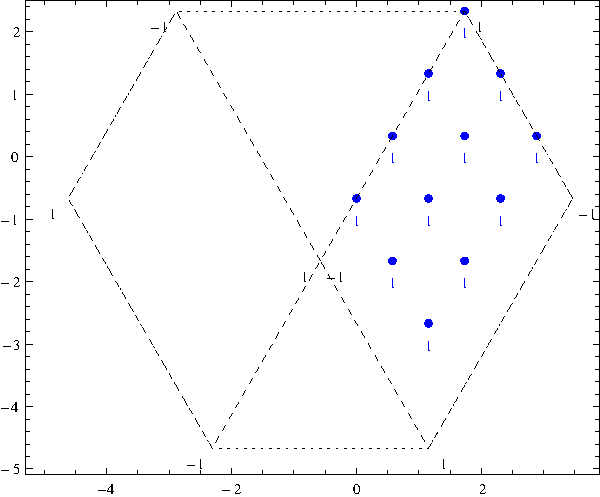
\includegraphics[width=80mm]{a2-a1}
  }
  \caption{Weyl group orbit (dotted) producing singular element of $L^{[3,2]}_{A_{2}}$ and its decomposition into the sum of splint images of singular elements of modules  $L^{[3,2]}_{A_{1}\oplus A_{1}}$ (dashed). Weight multiplicities of $L^{[3,2]}_{A_{1}\oplus A_{1}}$-module coincide with branching coefficients for the reduction $L^{[3,2]}_{A_{2}\downarrow A_{1}\oplus u(1)}$.}

 \label{fig:a2_splint}
\end{figure}
\end{example}
\begin{example}
  For the Lie algebra $B_{2}= \bf{so}(5)$ branching of its irreducible module $L^{[3,2]}$ into  modules of a reductive subalgebra $A_{1}\oplus u(1)$ with the root system spanned by the first simple root $\alpha_1=e_1-e_2$ of $B_{2}$. Singular element of $\Psi^{[3,2]}_{B_{2}}$ is decomposed into the sum of splint images of singular elements of $A_{2}$-modules and branching coefficients coincide with weight multiplicities of $A_{2}$-module (see Fig. \ref{fig:b2_splint}).

  \begin{figure}[h!bt]
  \hspace*{-1.2cm}

   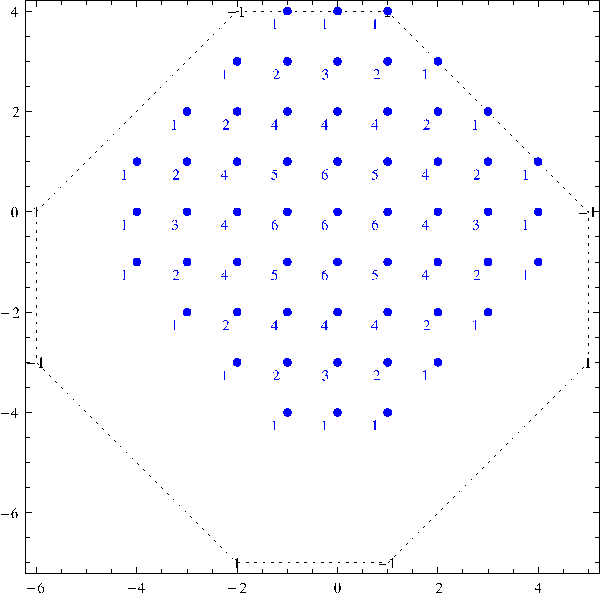
\includegraphics[width=65mm]{b2}
   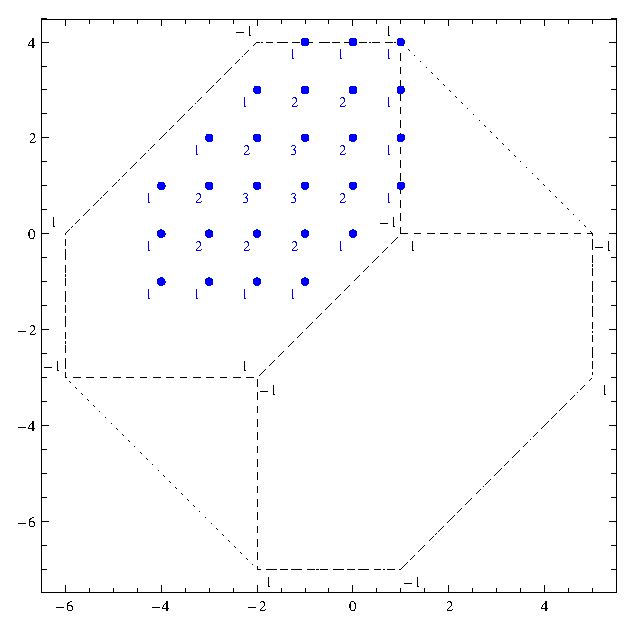
\includegraphics[width=65mm]{b2-a2-a1}
  \caption{Weights of the $B_{2}$-module $L^{[3,2]}$ are indicated by dots in the left picture (their multiplicities are also indicated). Contour of the singular element is shown by dotted line. The right picture presents the decomposition of  $\Psi_{B_{2}}(L^{[3,2]}_{B_{2}})$-singular element into the sum of splint images of singular elements $\Psi_{A_{2}}(L^{[3,2]})$ (dashed). Weight multiplicities of $L^{[3,2]}_{A_{2}}$-module coincide with branching coefficients for the reduction $L^{[3,2]}_{B_{2}\downarrow A_{1}\oplus u(1)}$.}

 \label{fig:b2_splint}
\end{figure}
\end{example}

\vspace{10mm}
\begin{example}
   Lie algebra $G_{2}$ has a regular subalgebra $A_{2}$ with root system $\Delta_{\mathfrak{a}}=\Delta_{A_{2}}$ containing the $G_{2}$ long roots. Consider branching of an irreducible module $L_{G_{2}}^{(3,2)}$ into the $A_{2}$-modules. Singular element $\Psi_{G_{2}}(L^{[3,2]})$ is decomposed into the sum of splint images of singular elements $\Psi_{A_{2}}(L^{[3,2]})$ and the corresponding branching coefficients coincide with weight multiplicities of $L^{[3,2]}_{A_{2}}$-module (see Fig. \ref{fig:g2_splint}).


  \begin{figure}[h!bt]
  \noindent\centering{
   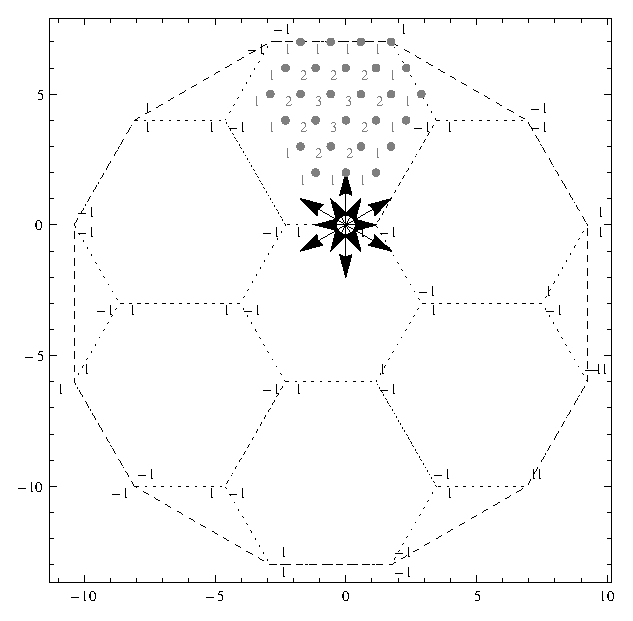
\includegraphics[width=120mm]{g2}
  }

  \caption{Weyl group orbit (dotted) for the singular element $\Psi_{G_{2}}(L^{[3,2]})$ and its decomposition into the sum of splint images of singular elements of $A_{2}$-modules (dashed). Weight multiplicities of $L^{[3,2]}_{A_{2}}$-module coincide with branching coefficients for the reduction $L^{[3,2]}_{G_{2}\downarrow A_{2}}$.}


 \label{fig:g2_splint}
\end{figure}

\end{example}

\section{Conclusions}

\label{sec:conclusions}It is explicitly demonstrated that splint
presents a very effective tool to find branching coefficients. In
particular injective splints provide a possibility to reduce
branching rules calculations for highest weight modules to a
determination of weight multiplicities for a module with the same
Dynkin labels referred to the Lie algebra $\mathfrak{s}$. This algebra
$\mathfrak{s}$ must not be a subalgebra in the initial $\mathfrak{g}$ , it
has the same rank $r_{\mathfrak{s}}=r$\ , but obviously less
"complicated" than $\mathfrak{g}$ -- only a subset of the initial root system is involved in the second stem $\Delta_{\mathfrak{s}}$.

It is significant that for the injections $D_{r}\hookrightarrow B_{r}$ , $%
D_{r}\hookrightarrow C_{r}$ and $A_{r-1}\oplus u\left( 1\right) \hookrightarrow A_{r}$ splint technique shows
transparently Gelfand-Tzeytlin rules for branching:  the reduction is
multiplicity free (all nonzero
branching coefficients are equal to 1). Here it is an immediate consequence of the
structure of the second stem being a direct sum of $A_{1}$
algebras and the fact that the corresponding module
$L_{\frak{s}}^{\mu }$ is irreducible.


%%%%%%%%%%%%%%%%%%%%%%%%%%%%%%%%%%%%%%%%%%%%%%%%%%%%%%%%%%%%%


%%%%%%%%%%%%%%%%%%%%%%%%%%%%%%%%%%%%%%%%%%%%%%%%%%%%%%%%%%%%%
\section*{Appendix}

%%%%%%%%%%%%%%%%%%%%%%%%%%%%%%%%%%%%%%%%%%%%%%%%%%%%%%%%%%%%%

Let us demonstrate that for injective splints of classical Lie
algebras the following property is valid:
\begin{Prop}
Let $\Delta \approx (\Delta _{\frak{a}},\Delta _{\frak{s}})$ be an
injective
splint with the decomposition of simple roots $S=S_{\frak{c}}\cup S_{\frak{d}%
}$ with $S_{\frak{c}}=S\cap S_{\frak{a}}$ and $S_{\frak{d}}=S\cap S_{\frak{s}%
}$.
\end{Prop}
Thus for any simple root $\beta \in S_{\frak{s}}$ there exists the
pair of
roots ( $\alpha $ ,$\beta ^{\prime }$) with $\alpha \in $ $S_{\frak{c}%
},\beta ^{\prime }\in S_{\frak{s}}$ such that $\alpha =\beta
-\beta ^{\prime }$

\begin{itemize}
\item
Type 1. $\Delta _{G_{2}}\approx (\Delta _{A_{2}},\Delta
_{A_{2}}).$

 \begin{figure}[h!bt]
  \noindent\centering{
   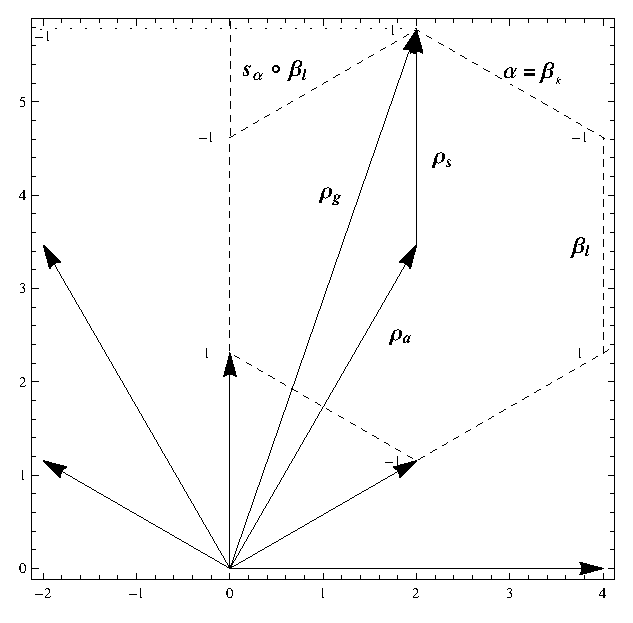
\includegraphics[width=100mm]{g2-roots}
  }
  \caption{Positive roots of $G_{2}$ and formation of singular element $\Phi^{(0)}_{\mathfrak{s}}$ in the main Weyl chamber of $\mathfrak{a}=A_{2}$.}
\end{figure}
Here both stems are metric and the corresponding root systems are
equivalent. In Figure 4 a part of the singular element $\Phi
_{G_{2}}^{\left( 0\right) }$ is presented. The boundaries of $\bar{C_{\frak{a%
}}}$ are the dashed lines starting at the center of the singular
element. It
contains the edge $\lambda _{2}=-\alpha _{2}=-\beta _{2}$ and the roots $%
-\beta _{1}=-s_{\alpha _{2}}\circ \beta _{3}$ and $ -\beta _{3}$
($\beta _{3}$ is indicated as $\beta _{l}$). For the root $\beta
_{1}$ the necessary pair
is  $(\alpha _{1}, \beta _{2})$: $\alpha _{1}=\beta _{1}-\beta _{2}$. The $%
\lambda _{2,3}^{\frak{s}}=\beta _{3}$ edge is equal to $\lambda _{1}^{\frak{s%
}}=\beta _{1}=s_{\alpha _{2}}\circ \beta _{3}$ and $m_{1}$ index
is aquired by the $\frak{s}$-module that also inherit the second
index $m_{2}$. In this particular
case they are $m_{1}=m_{2}=0$. The general case with the initial module $%
L^{\mu }$ and $\mu =m_{1}\omega _{1}+m_{2}\omega _{2}$ can be
treated in the same way: one finds an edge $\lambda _{2}=-\left(
m_{2}+1\right) \beta _{2}$ and put $\lambda
_{1}^{\frak{s}}=-\left( m_{1}+1\right) \beta _{1}$, its end
belongs to the boundary $\bar{C_{\frak{a}}}$. The reflection
$s_{\beta
_{2}} $ sends $\beta _{1}$ to $\beta _{3}$ and the corresponding edge 
$\lambda _{2,3}^{\frak{s}}=-\left( m_{1}+1\right) \beta _{3}$ has
the length $\left( m_{1}+1\right) $. Now consider $\lambda _{1}^{\frak{s}}$ (or
$\lambda _{2,3}^{\frak{s}} $) and $\lambda _{1,3}^{\frak{s}}$ (or
$\lambda _{2,3,1}^{\frak{s}}$) edges to find that they belong to
the boundary $\bar{C_{\frak{a}}}$ and the Weyl symmetry predicts
that $\lambda _{1,3}^{\frak{s}}=-\left( m_{2}+1\right)
\beta _{3}$ ($\lambda _{2,3,1}^{\frak{s}}=-\left( m_{2}+1\right) \beta _{1}$%
) . Finally the edge $\lambda _{1,3,2}^{\frak{s}}=-\left(
m_{1}+1\right) \beta _{2}$ closes the polytope. Its vertices
correspond to weights of the singular
element $\Phi _{\frak{s}}^{\left( \widetilde{\mu }\right) }=\sum_{w\in W_{%
\frak{s}}}\varepsilon \left( w\right) e^{w\circ \left(
\widetilde{\mu }+\rho
_{\frak{s}}\right) }$ of the module $L_{\frak{s}}^{\left( \widetilde{\mu }%
\right) }$ with $\widetilde{\mu }=m_{1}\widetilde{\omega }_{1}+m_{2}%
\widetilde{\omega }_{2}$. Notice that in this case the sign
factors can be obtained directly in the initial weight system as
far as the stem is metric.
\item
Type 1. $\Delta _{F_{4}}\approx (\Delta _{D_{4}},\Delta
_{D_{4}}).$

Both stems are metric here and the corresponding root systems are
equivalent. The system $\Delta _{D_{4}}$ of the subalgebra
$\frak{a=}D_{4}$ is formed by the set $\left\{ \pm e_{i}\pm
e_{j}\right\} _{|i,j=1,\ldots 4,\; i\neq j}.$ The simple roots
$S_{\frak{c}}$ are $\left\{ e_{2}-e_{3},e_{3}-e_{4}\right\} $ and
$S_{\frak{d}}=\left\{ e_{4},\frac{1}{2}\left(
e_{1}-e_{2}-e_{3}-e_{4}\right) \right\} $.
For a module $L^{\mu }$ with $\mu =\sum m_{k}\omega _{k}$ consider the edge $%
\lambda _{3}=-\left( m_{3}+1\right) e_{4}=-\left( m_{3}+1\right)
\beta _{3}$.
 Compose an edge $\lambda _{2}^{\frak{s}}=-\left( \widetilde{m}%
_{2}+1\right) \beta _{2}$. The necessary pair of roots is $\left(
\alpha
_{2}=e_{3}-e_{4},\beta _{3}\right) $. The intersection of $\lambda _{2}^{%
\frak{s}}$ with the $\alpha _{2}$-boundary of
$\bar{C_{\frak{a}}}$ fixes
its length to be $\lambda _{2}^{\frak{s}}=-\left( m_{2}+1\right) \beta _{2}$%
\ and the length of the edge $\lambda _{3,2}^{\frak{s}}$ is equal
to that of
$\lambda _{2}^{\frak{s}}$. Next consider the edge $\lambda _{2}^{\frak{s}%
}=-\left( m_{2}+1\right) \beta _{2}$ and the pair $\left( \alpha
_{1}=e_{2}-e_{3},\beta _{1}=e_{2}\right) $. The length of  
$\lambda _{1}^{\frak{s}}$ becomes equal to $\lambda
_{1}^{\frak{s}}=-\left( m_{1}+1\right) \beta _{1}$. Proceed further till the closure of the polytope. 
The edges looking along the roots of the $\alpha_4$-type, $\alpha _{4}=\beta
_{4}=$ $\frac{1}{2}\left( e_{1}-e_{2}-e_{3}-e_{4}\right) $, are
treated similarly and finally the singular element $\Phi
_{\frak{s}}^{\left( \widetilde{\mu }\right) }=\sum_{w\in
W_{\frak{s}}}\varepsilon \left( w\right) e^{w\circ \left(
\widetilde{\mu }+\rho _{\frak{s}}\right) }$ for the module
$L_{\frak{s}}^{\left( \widetilde{\mu }\right) }$ with
$\widetilde{\mu }=\sum m_{k}\widetilde{\omega }_{k}$ is formed in
$\bar{C_{\frak{a}}}$.
\item
Type 2. $\Delta _{B_{r}}\approx (\Delta _{D_{r}},\Delta _{\oplus
^{r}A_{1}}). $

Both stems are metric. An injection is fixed by the stem $\Delta
_{D_{r}}$ simple roots $S_{\frak{a}}=\left\{
e_{1}-e_{2},e_{2}-e_{3},\ldots
,e_{r-1}-e_{r},e_{r-1}+e_{r}\right\} $. The second stem
corresponds to a
direct sum of algebras $A_{1}$ with the simple roots $S_{\frak{s}%
}=\left\{ e_{1},e_{2},\ldots ,e_{r-1},e_{r}\right\} $. Consider the edge $%
\lambda _{r}=-\left( m_{r}+1\right) \beta _{r}$ (here $\beta
_{r}=e_{r}$) and $\lambda _{r-1}=-\left(
\widetilde{m}_{r-1}+1\right) \beta _{r-1}$
attached to it (here $\beta _{r-1}=e_{r-1}$). The corresponding pair is $%
\left( \alpha _{r-1}=e_{r-1}-e_{r},\beta _{r-1}=e_{r-1}\right) $.
 The intersection condition fixes the second edge to be $\lambda
_{r-1}=-\left( m_{r-1}+1\right) \beta _{r-1}$ , it is orthogonal
to $\beta _{r}$ so the opposite edge has the same length. The
Dynkin index $m_{r-1}$ now refers
also to the\ simple root $\beta _{r-1}$. Next consider the obtained edge $%
\lambda _{r-1}=-\left( m_{r-1}+1\right) \beta _{r-1}$ and $\lambda
_{r-2}=-\left( \widetilde{m}_{r-2}+1\right) \beta _{r-2}$ to
fix the index $\widetilde{m}_{r-2}=m_{r-2}$ and the edge
$\lambda _{r-2}=-\left( m_{r-2}+1\right) \beta _{r-2}$ and so on
till all the pairs of edges are properly fixed. Finally in
$\bar{C}_{D_{r}}$ the element $\Phi _{\oplus ^{r}A_{1}}^{\left(
\widetilde{\mu }\right) }=\sum_{w\in W_{\oplus
^{r}A_{1}}}\varepsilon \left( w\right) e^{w\circ \left( \widetilde{\mu }+%
\frac{1}{2}\sum e_{k}\right) }$ can be constructed for the module
$L_{\oplus ^{r}A_{1}}^{\left( \widetilde{\mu }\right) }$ with
$\widetilde{\mu }=\sum m_{k}\frac{1}{2}e_{k}$.

\item
Type 2. $\Delta _{C_{r}}\approx (\Delta _{D_{r}},\Delta _{\oplus
^{r}A_{1}}). $

The situation in this case is eqivalent to the previous one and
the additional edges are constructed similarly.
\item
Type 3 $\Delta _{A_{r}}\approx (\Delta _{A_{r-1}\oplus
u_{1}},\Delta _{\oplus ^{r}A_{1}}).$

Here only the first stem is metric and it fixes the injection with
simple roots $S_{\frak{a}}=\left\{ e_{1}-e_{2},e_{2}-e_{3},\ldots
,e_{r-1}-e_{r}\right\} $. The second stem corresponding to a direct sum of $%
r$ copies of $A_{1}$ has the simple roots $S_{\frak{s}}=\left\{
e_{1}-e_{r+1},e_{2}-e_{r+1},\ldots ,e_{r}-e_{r+1}\right\} $.
Consider the edge $\lambda _{r}=-\left( m_{r}+1\right) \beta _{r}$
with $\beta
_{r}=e_{r}-e_{r+1}$ and $\lambda _{r-1}=-\left( \widetilde{m}%
_{r-1}+1\right) \beta _{r-1}$ \ with $\beta
_{r-1}=e_{r-1}-e_{r+1}$ attached to it. Then the corresponding
pair is $\left( \alpha _{r-1}=e_{r-1}-e_{r},\beta
_{r-1}=e_{r-1}-e_{r+1}\right)$. The intersection with the
boundary of $\bar{C}_{A_{r-1}}$ orthogonal to $\alpha _{r-1}$
fixes the second edge to be $\lambda _{r-1}=-\left(
m_{r-1}+1\right) \beta _{r-1}$. The Dynkin index $m_{r-1}$ is to
be used for the fundamental weight  $\omega _{r-1}.$ The\
reflection $s_{\beta _{r}}$ sends $\lambda _{r-1}=-\left(
m_{r-1}+1\right) \beta _{r-1}$ to $\lambda _{r,r-1}=-\left(
m_{r-1}+1\right) \beta _{r-1}.$ Next consider the obtained edge
$\lambda _{r-1}=-\left( m_{r-1}+1\right) \beta _{r-1}$ and
$\lambda _{r-2}=-\left( \widetilde{m}_{r-2}+1\right) \beta _{r-2}$
with $\beta _{r-2}=e_{r-2}-e_{r+1} $ to obtain the index
$\widetilde{m}_{r-2}=m_{r-2}$ and the edge $\lambda _{r-2}=-\left(
m_{r-2}+1\right) \beta _{r-2}$ and so on till all the pairs of
edges are properly fixed. Finally in $\bar{C}_{D_{r}}$ the element
$\Phi _{\oplus ^{r}A_{1}}^{\left( \widetilde{\mu }\right)
}=\sum_{w\in W_{\oplus
^{r}A_{1}}}\varepsilon \left( w\right) e^{w\circ \left( \widetilde{\mu }+%
\widetilde{\rho }\right) }$ can be constructed for the module
$L_{\oplus ^{r}A_{1}}^{\left( \widetilde{\mu }\right) }$ with
$\widetilde{\mu }=\sum m_{k}\beta _{k}.$ The simplest case
$\Delta _{A_{2}}\approx (\Delta _{A_{1}\oplus u_{1}},\Delta
_{A_{1}\oplus A_{1}})$ is presented in Example 4.1 and Figure 1.
\item
Type 3 $\Delta _{B_{2}}\approx (\Delta _{A_{1}},\Delta _{A_{2}}).$

This splint is illustrated in Example 4.1 and Figure 1, 
$S_{A\_1}=\left\{ e_{1}-e_{2}\right\} $, $S_{A\_2}=\left\{
e_{1},e_{2}\right\} $. The edge $\lambda _{\alpha _{2}}=\lambda
_{\beta _{2}}=-\left( m_{2}+1\right) \beta _{2}$ is followed by
$\lambda _{\beta _{1}}=-\left( \widetilde{m}_{1}+1\right) \beta
_{1}$. Consider the pair $\left( \alpha
_{1}=e_{1}-e_{2},\beta _{1}=e_{1}\right)$. The end of the edge
$\lambda _{\beta _{1}}$ must indicate a weight
invariant under the reflexion $s_{\alpha _{1}}$.  Its length is thus fixed: 
$\lambda _{\beta _{1}}=-\left( m_{1}+1\right) \beta _{1}$. In the
coimage of
the second stem, that is in the root system $\Delta_{A_{2}}$, the reflection 
$s_{\beta _{2}}$ sends $\lambda _{\beta _{1}}=-\left(
m_{1}+1\right) \beta
_{1}$ to $\lambda _{2,3}$, thus the latter edge has the same length in $%
\beta _{3}=e_{1}+e_{3}$, we have $\lambda _{2,3}=-\left(
m_{1}+1\right)
\beta _{3}$ with $\beta _{3}=e_{1}+e_{3}$. The irreducible $\frak{s}$%
-module has the highest weight $\widetilde{\mu }=m_{1}\widetilde{\omega }%
_{1}+m_{2}\widetilde{\omega }_{2}$. In Figure 1 we see the
details of these relations in a particular case where
$L_{B_{2}}^{\left[ 3,2\right] }$ is reduced to a subalgebra
$A_{1}\oplus u\left( 1\right) $ and the
corresponding highest weights (with their multiplicities) form the diagram $%
\mathcal{N}_{A_2}^{\left[ 3,2\right] }$ .
\end{itemize}

%%%%%%%%%%%%%%%%%%%%%%%%%%%%%%%%%%%%%%%%%%%%%%%%%%%%%%%%%%%%%
%%%%%%%%%%%%%%%%%%%%%%%%%%%%%%%%%%%%%%%%%%%%%%%%%%%%%%%%%%%%%


\section{Выводы к первой главе}


%%
%% End of file
%%% Local Variables: 
%%% mode: latex
%%% TeX-master: "thesis"
%%% End: 
